\subsection{Semi-Leptonic} \label{sec:SL_Selections}

Events fall into the Semi-Leptonic analysis category if they contain at least one pre-selected diphoton as described in Section \ref{sec:photons}, and contain 
exactly one lepton passing the common lepton selections described in Section \ref{sec:LeptonSelections}. The Semi-Leptonic channel is expected to be the most 
sensitive of the three WW$\gamma\gamma$ channels due to the combination of a relatively large $W\rightarrow qq$ branching ratio of $\approx$ 67\%, and the presence of a clean, highly energetic 
lepton from the $W\rightarrow\ell\nu$ decay leg. 

The four NLO generated Semi-Leptonic signal events corresponding to the points $\kappa_{\lambda}$ = [0, 1 (SM), 2.45, 5], and a set of samples coming from a reweighting of these four samples to the points $3D3$ ($\kappa_{\lambda}$ = 0, $\kappa_{t}$ = 1.0, $c_{ttHH}$ = 1.0), $c_{ttHH}$ = 3, and $c_{ttHH}$ = 0.35 are categorized with a multi-class DNN, where $c_{ttHH}$ represents the coupling strength of two top quarks to two Higgs bosons. These corresponding simulation templates are used to model the Semi-Leptonic HH final state for the SM hypothesis, and to perform scans of the $\kappa_{\lambda}$ and $c_{2}$ EFT parameters. 

The four generated NLO samples are reweighted to the 20 EFT benchmarks, and categorized using a parametric DNN which includes the EFT benchmark scenario number as a training variable. The resulting categorized simulation templates are used to model the semi-leptonic HH final state for these 20 scenarios. 

\subsubsection{Standard Model: Multiclass Deep Neural Network}

For a general description of Deep Neural Networks, see Appendix \ref{sec:DNN}. 

In the Semi-Leptonic category, in order to separate the di-Higgs signal from the expected single Higgs boson and continuum backgrounds, a multiclass deep neural network is trained to identify these three types of processes 
separately, in order to identify regions of phase space with a maximal number of HH events, but a minimal number of single H and continuum background events. Because the single higgs and continuum background 
processes are markedly different due to the expectation of a resonant H signal vs. a falling continuum background, as shown in Figure \ref{fig:Signatures}, it is more logical to define these two processes separately in a DNN training rather 
than defining them as the same type of background. 

% The multiclass DNN is trained using 2017 signal and background samples, and is evaluated on 2016, 2017 and 2018 signal samples for analytic fitting, and on Run 2 CMS data 
% to be used for categorization and data-driven background modeling. The 12 generated LO EFT benchmark samples, as well as the LO SM benchmark, are reweighted to the SM HH process at NLO and are combined and considered together as 
% signal in the training.

% The network is trained on a labelled dataset where the 2017 HH process is defined as signal, and single higgs and non-Higgs datasets which are defined as separate classes. The single higgs processes
% trained on are the associated VH and ttH production modes of $H\rightarrow\gamma\gamma$.

The samples used for training and labeled as signal are the 12 LO benchmark samples, as well as the LO SM benchmark, where all thirteen simulation samples include 2017 detector conditions for reconstruction. When training on these 
samples, the reweighting procedure described in Section \ref{sec:EFT_Description}
is applied to reweight these LO EFT benchmark and SM sample to the SM process at NLO, in order to train the network to identify the SM at NLO HH signal. 
In deriving these weights, NLO samples are reweighted following \cite{Buchalla:2018yce}, and LO samples are reweighted 
following an analytic parameterization as a function of $\sigma_{HH}$ and $|\cos{\theta^*}|$ which extends beyond $m_{HH} = 1050$ GeV, and the ratio of the two is taken 
and normalized by Equation \ref{eq:LONLONorm}, yielding an event by event weight. These event weights scale the per-event training loss in order to 
assign more training importance to events which must be weighted up in order to match SM NLO. 

The ratio of a few of the DNN's input variable distributions between the sum of reweighted 13 LO benchmarks (12 + SM at LO), and the 2017 SM at NLO signal are shown in Figures \ref{fig:LO_NLO_Reweight_CrPlts-1} and \ref{fig:LO_NLO_Reweight_CrPlts-2}, and the rest are shown in Appendix \ref{sec:DNN-Input-Variables-LO_NLO_Weight_Validation}.

\begin{figure}[h!]
    \setcounter{subfigure}{0}
    \centering
    \subfloat[Scaled Leading Photon \pt]{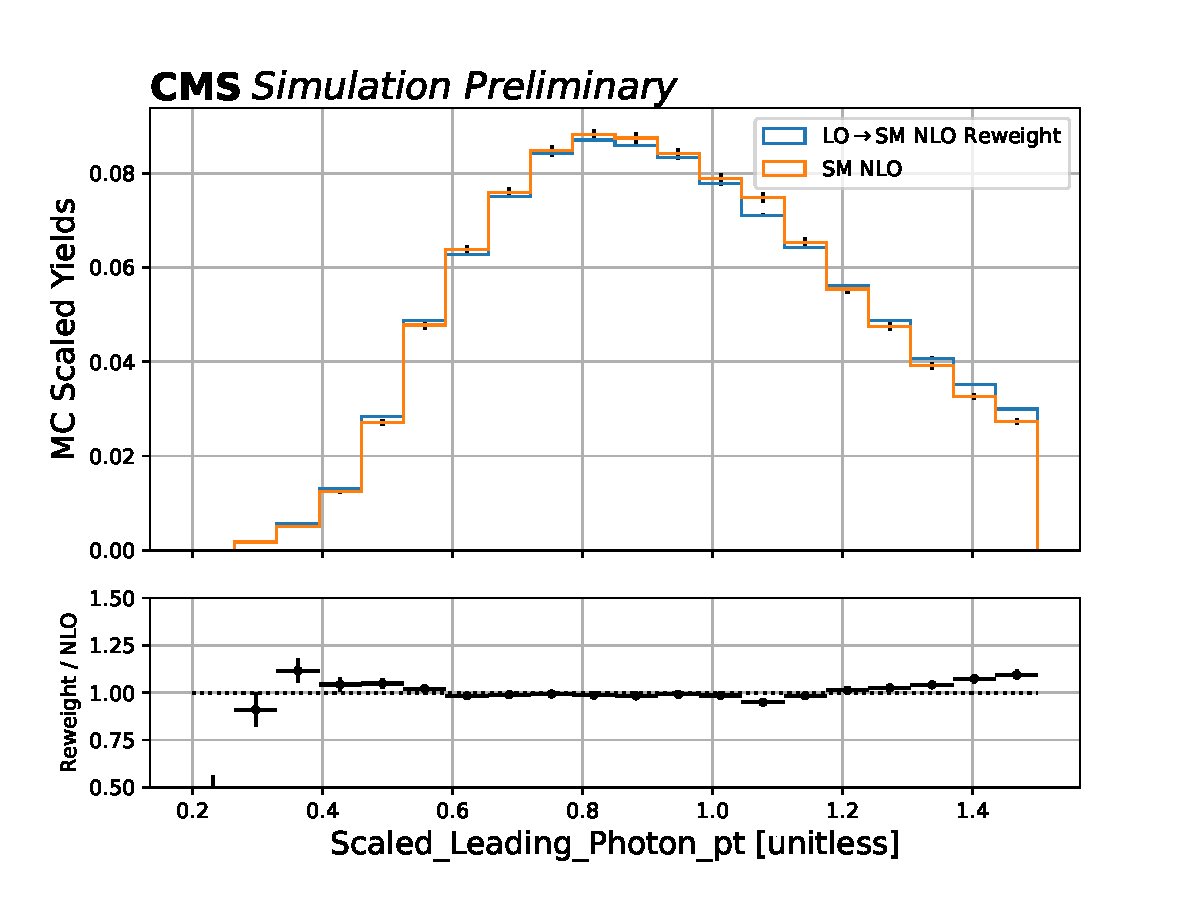
\includegraphics[width=0.475\textwidth]{Sections/HHWWgg/images/DNN/LO_NLO_Reweight_Distributions/Scaled_Leading_Photon_pt.pdf}}
    \subfloat[Scaled subleading photon \pt]{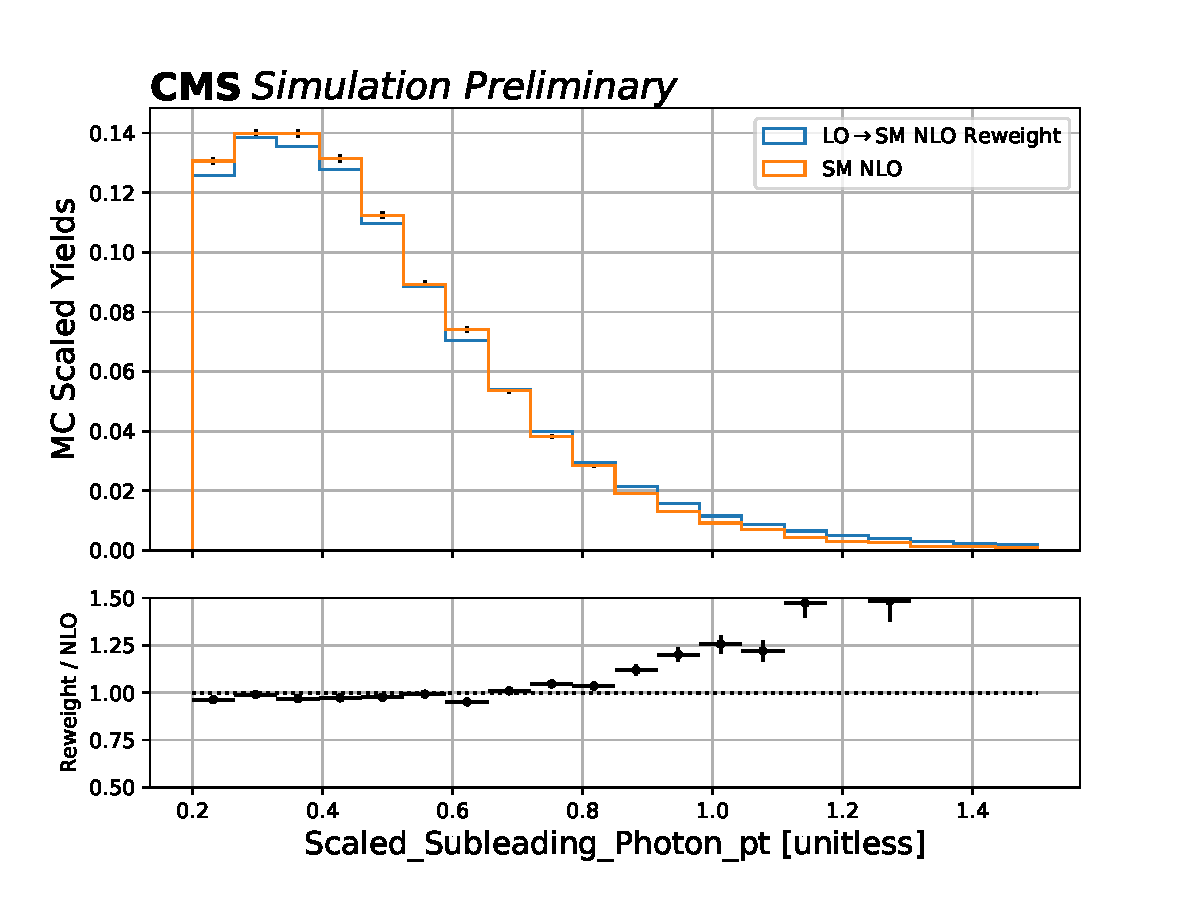
\includegraphics[width=0.475\textwidth]{Sections/HHWWgg/images/DNN/LO_NLO_Reweight_Distributions/Scaled_Subleading_Photon_pt.pdf}}
    \caption{Scaled leading and subleading photon \pt. \label{fig:LO_NLO_Reweight_CrPlts-1}}
\end{figure}
    
\begin{figure}[h!]
    \setcounter{subfigure}{0}
    \centering
    \subfloat[Lepton $p_{T}$]{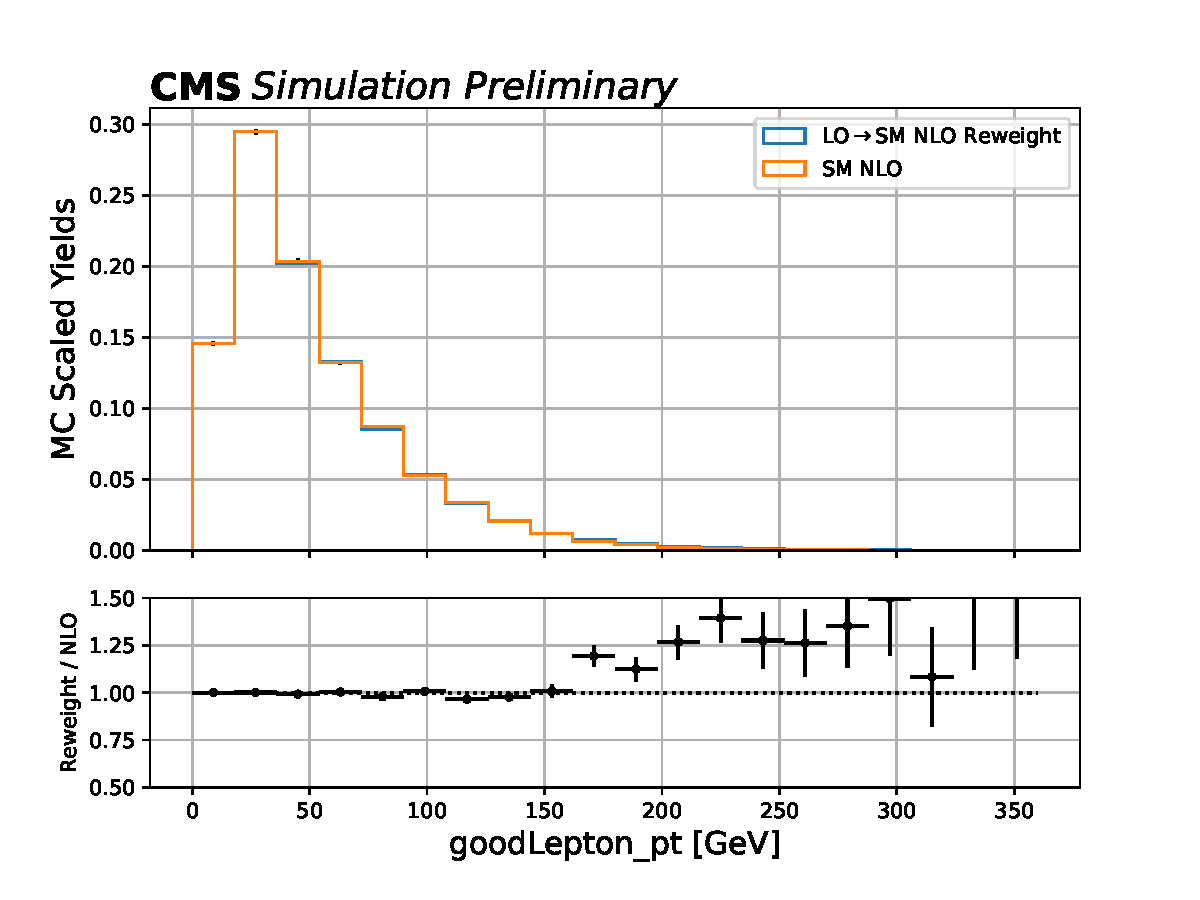
\includegraphics[width=0.475\textwidth]{Sections/HHWWgg/images/DNN/LO_NLO_Reweight_Distributions/goodLepton_pt.pdf}}
    \subfloat[MET]{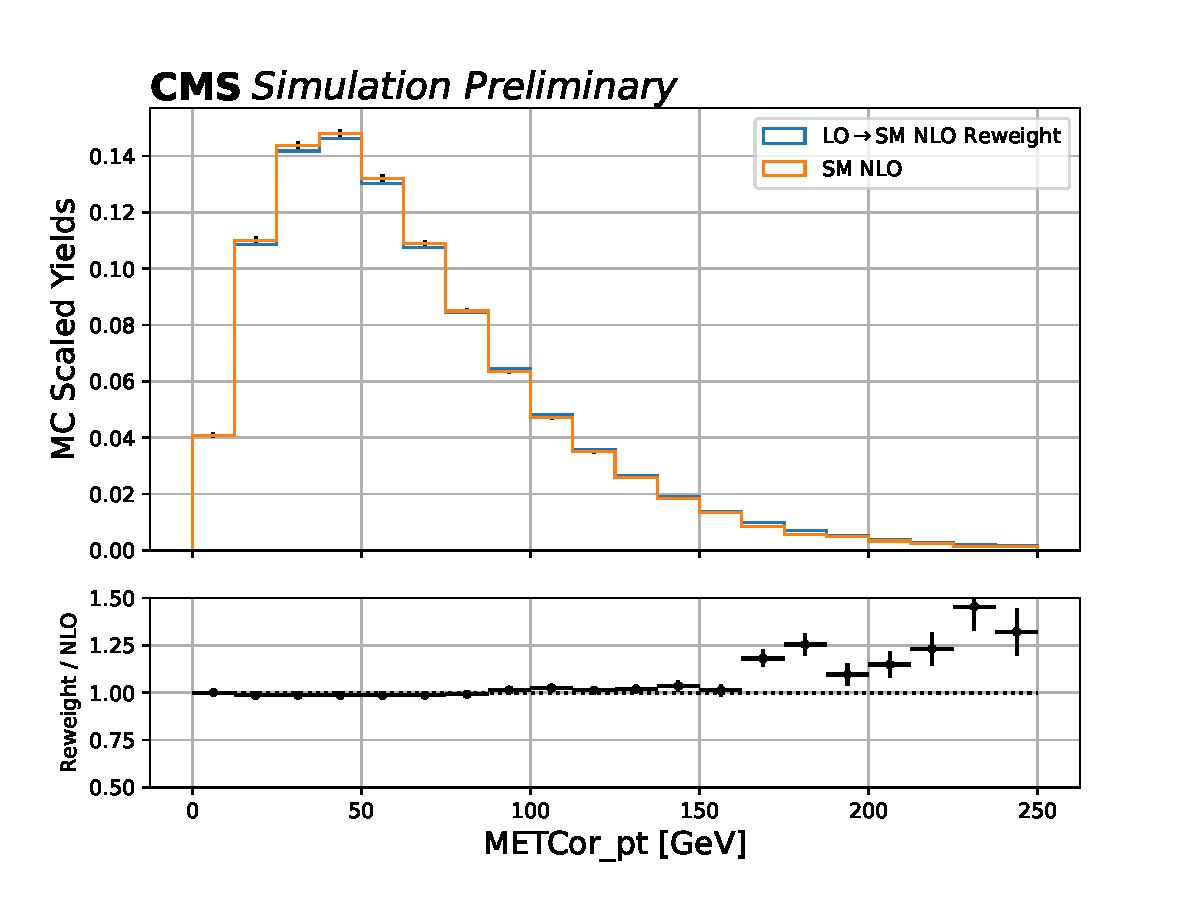
\includegraphics[width=0.475\textwidth]{Sections/HHWWgg/images/DNN/LO_NLO_Reweight_Distributions/METCor_pt.pdf}}
    \caption{Lepton \pt and MET\label{fig:LO_NLO_Reweight_CrPlts-2}}
\end{figure}

There is good agreement overall, indicating that training on these events and including the LO to NLO event reweighting in the training via loss scaling trains a network geared towards identifying the SM and NLO signal.

The samples used for training and labeled as single Higgs processes are the associated production of a Higgs boson with a vector boson (VH), and with a top quark pair (ttH), where the Higgs decays to $\gamma\gamma$ in both cases. 

The samples used for training and labeled as continuum background were chosen based on the background MC processes which have at least 1000 absolute events after the semi-leptonic pre-selections, such that there is no large statistical uncertainty on these process descriptions. 

Events used to train the network are required to contain at least one diphoton candidate passing the common diphoton selections described in Section \ref{sec:photons},
and contain exactly one lepton passing the common lepton selections in Section \ref{sec:LeptonSelections}.

Due to the class imbalance in the datasets, events are re-weighted with a per-class ``class weight", such that after applying this weight, the effective number 
of events in both classes is the same. In deriving each class weight, a class's weighted MC yield is scaled to the unweighted HH yield of 866,833. This ensures that the network focuses on categorizing all three classes with equal importance. The unweighted and weighted yields, 
and class weights of all training events which have only diphoton pre-selections applied and the requirement of exactly one lepton passing the common lepton selections, 
are shown in Table \ref{tab:yieldsAndClassWeights}. Note that 
in Table \ref{tab:yieldsAndClassWeights}, HH events are not normalized to cross section and branching ratio,
as this is not necessary because all weighted yields are reweighted to a common target, and therefore what is relevant are the relative yields. 

\begin{figure}[H]
        \resizebox{1\textwidth}{!}{%
          \begin{tabular}{c|c|c|c|c} 
                  Class & Unweighted Yield & Weighted Yield & Class Weight & Class Weight * Weighted Yield \\ \hline
                   HH & 866833 & 2.232871 & 388214 & 866833 \\
                   H & 78108 & 1.057757 & 819501 & 866833 \\
                   Continuum Background & 61408 & 16104 & 53.8278 & 866833 \\ \hline 
          \end{tabular}}
        \captionof{table}{Unweighted and weighted yields, and class weights applied during Semi-Leptonic DNN training, without data sideband scale. Weighted class yields are reweighted by class weights to the unweighted HH yield. \label{tab:yieldsAndClassWeights}}
        
\end{figure}

The features used as input to the semi-leptonic channel DNN can be found in Table \ref{tab:SLinputvars}. 

\begin{table}[H]
\caption{Input features used to train semi-leptonic channel DNN.}
\resizebox{\textwidth}{!}{
\begin{tabular}{| l | l |}
\hline
Feature & Description \\
\hline
Leading Photon p$_T$ / \mgg& Transverse momentum of the photon with the highest transverse momentum out of the selected photons, scaled to diphoton mass. \\
Leading Photon $\eta$ & Pseudorapidity of the photon with the highest transverse momentum out of the selected photons \\
Leading Photon $\phi$ & Direction in the transverse plane of the photon with the highest transverse momentum out of the selected photons \\
Leading Photon E / \mgg& Energy of the photon with the highest transverse momentum out of the selected photons, scaled to diphoton mass. \\
Leading Photon MVA & Photon MVA score of the photon with the highest transverse momentum out of the selected photons \\
Subleading Photon p$_T$  / \mgg& Transverse momentum of the photon with the second highest transverse momentum out of the selected photons, scaled to diphoton mass. \\
Subleading Photon $\eta$ & Pseudorapidity of the photon with the second highest transverse momentum out of the selected photons \\
Subleading Photon $\phi$ & Direction in the transverse plane of the photon with the second highest transverse momentum out of the selected photons \\
Subleading Photon E / \mgg & Energy of the photon with the second highest transverse momentum out of the selected photons, scaled to diphoton mass. \\
Subleading Photon MVA & Photon MVA score of the photon with the second highest transverse momentum out of the selected photons \\
Jet Multiplicity & Number of selected jets in the event (flavour inclusive) \\
Leading Jet p$_T$ & Transverse momentum of the jet with the highest transverse momentum out of the selected jets \\
Leading Jet $\eta$ & Pseudorapidity of the jet with the highest transverse momentum out of the selected jets \\
Leading Jet $\phi$ & Direction in the transverse plane of the jet with the highest transverse momentum out of the selected jets \\
Leading Jet E & Energy of the jet with the highest transverse momentum out of the selected jets \\
Leading Jet DeepJet Score & DeepJet b-tag discriminator score of the jet with the highest transverse momentum out of the selected jets \\
Subleading Jet p$_T$ & Transverse momentum of the jet with the second highest transverse momentum out of the selected jets \\
Subleading Jet $\eta$ & Pseudorapidity of the jet with the second highest transverse momentum out of the selected jets \\
Subleading Jet $\phi$ & Direction in the transverse plane of the jet with the second highest transverse momentum out of the selected jets \\
Subleading Jet E & Energy of the jet with the second highest transverse momentum out of the selected jets \\
Subleading Jet DeepJet Score & DeepJet b-tag discriminator score of the jet with the second highest transverse momentum out of the selected jets \\
Lepton p$_{T}$ & Transverse momentum of the selected lepton \\ 
Lepton $\eta$ & Pseudorapidity of the selected lepton \\ 
Lepton $\phi$ & Direction in the transverse plane of the selected lepton \\ 
Lepton E & Energy of the selected lepton \\ 
MET & The missing transverse energy \\ 
$M_{T}$(l, MET) & The transverse mass of the selected lepton and MET \\
$m_{j_{0},j_{1}}$ & The invariant mass of the leading and subleading jets \\ 
\hline
\end{tabular}
}
\label{tab:SLinputvars}
\end{table}

To determine the level of optimization of the network towards CMS data by training on MC, the data-MC ratio is checked for input features in the data sideband region after the semi-leptonic preselections are applied. Disagreements are seen between data and MC in the data sideband (100 $<$ $\mgg$ $<$ 115 or 135 $<$ $\mgg$ $<$ 180 GeV), as shown for various input features shown 
in Figures \ref{fig:Kin_Reweight_0_withoutKinWeights}, 
\ref{fig:Kin_Reweight_1_withoutKinWeights}, \ref{fig:Kin_Reweight_2_withoutKinWeights}, \ref{fig:Kin_Reweight_3_withoutKinWeights}, \ref{fig:Kin_Reweight_4_withoutKinWeights}, and
\ref{fig:Kin_Reweight_5_withoutKinWeights}. In
order to improve data/MC agreement so that the input features of the DNN are closer to a representation of the data in order to train a DNN more optimally, a 6-dimensional kinematic reweighting is performed. 

A per-event weight, called a kinematic weight, is computed as the ratio between data and background MC from the $\mgg$ sideband region (Note that data events in the signal region, 115 $<$ $\mgg$ $<$ 135 GeV, are not used at all when deriving
the kinematic weights). The variables Leading Jet \pt, Subleading Jet \pt, Lepton \pt, 
Leading Photon \pt over \mgg, Subleading Photon \pt over \mgg, and MET are used to calculate this per-event weight, as they correspond to quantities related to the semi-leptonic WW$\gamma\gamma$ final state particles. During the derivation of the weights, 5 bins are used for each variable. The range of each 
bin is selected in an automatic way such that there are the same number of data events in each bin. When the number of data events in a bin is lower than 20, the kinematic weight is set to 1. Otherwise,
the weight is set equal to the ratio (data entries)/(MC entries). 
After the kinematic weights are derived, a fiducial selection is made removing all events 
which have $|w_{MC}*w_{k}| > 10$, where $w_{MC}$ is the nominal MC weight computed from cross section, luminosity, PU weight, scale factors and GEN weights, and $w_{k}$ represents the per event kinematic weight. 
This fiducial selection removes events with very large weights which heavily impact the DNN training in a non-desirable way. 

The data/MC after applying the per-event kinematic weights, in the data sideband (100 $<$ $\mgg$ $<$ 115 or 135 $<$ $\mgg$ $<$ 180 GeV) and before any evaluation of the DNN, are shown in Figures \ref{fig:Kin_Reweight_0_withKinWeights}, 
\ref{fig:Kin_Reweight_1_withKinWeights}, \ref{fig:Kin_Reweight_2_withKinWeights}, \ref{fig:Kin_Reweight_3_withKinWeights}, \ref{fig:Kin_Reweight_4_withKinWeights}, \ref{fig:Kin_Reweight_5_withKinWeights}. It can be 
seen that the application of the kinematic weights improves the data/MC agreement, especially in very high yield bins. It can also be seen that after applying the kinematic reweighting there is no 
introduction of extremely large statistical uncertainties or fluctuations, indicating that there is a sufficient amount of data and MC events in deriving the kinematic weights. 

\newpage 

\begin{figure}[h!]
    \setcounter{subfigure}{0}
    \centering
    \subfloat[Before kinematic reweighting applied]{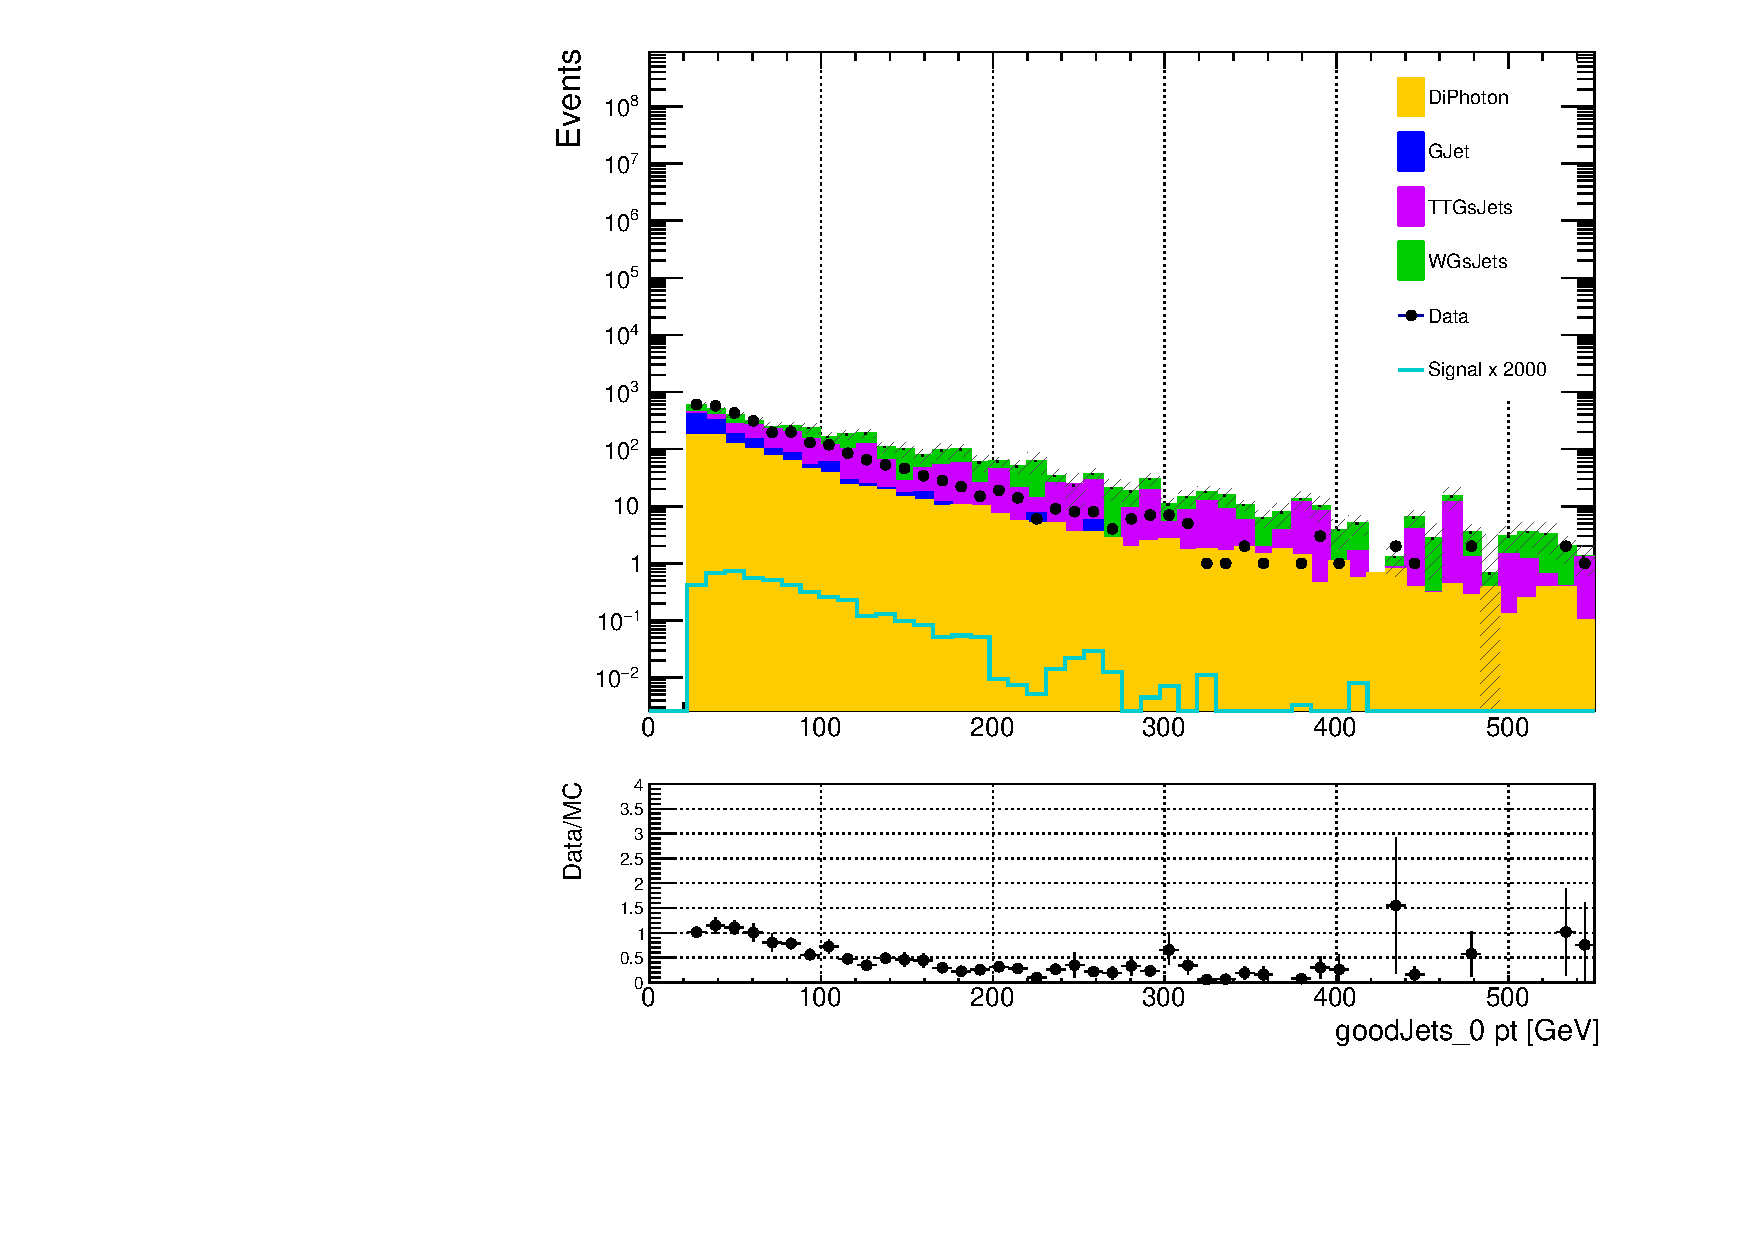
\includegraphics[width=0.45\textwidth]{Sections/HHWWgg/images/Semileptonic_Kinematic_Reweighting/Data_MC_WithoutKinWeights/goodJets_0_pt_log.pdf}\label{fig:Kin_Reweight_0_withoutKinWeights}} 
    \qquad     
    \subfloat[After kinematic reweighting applied]{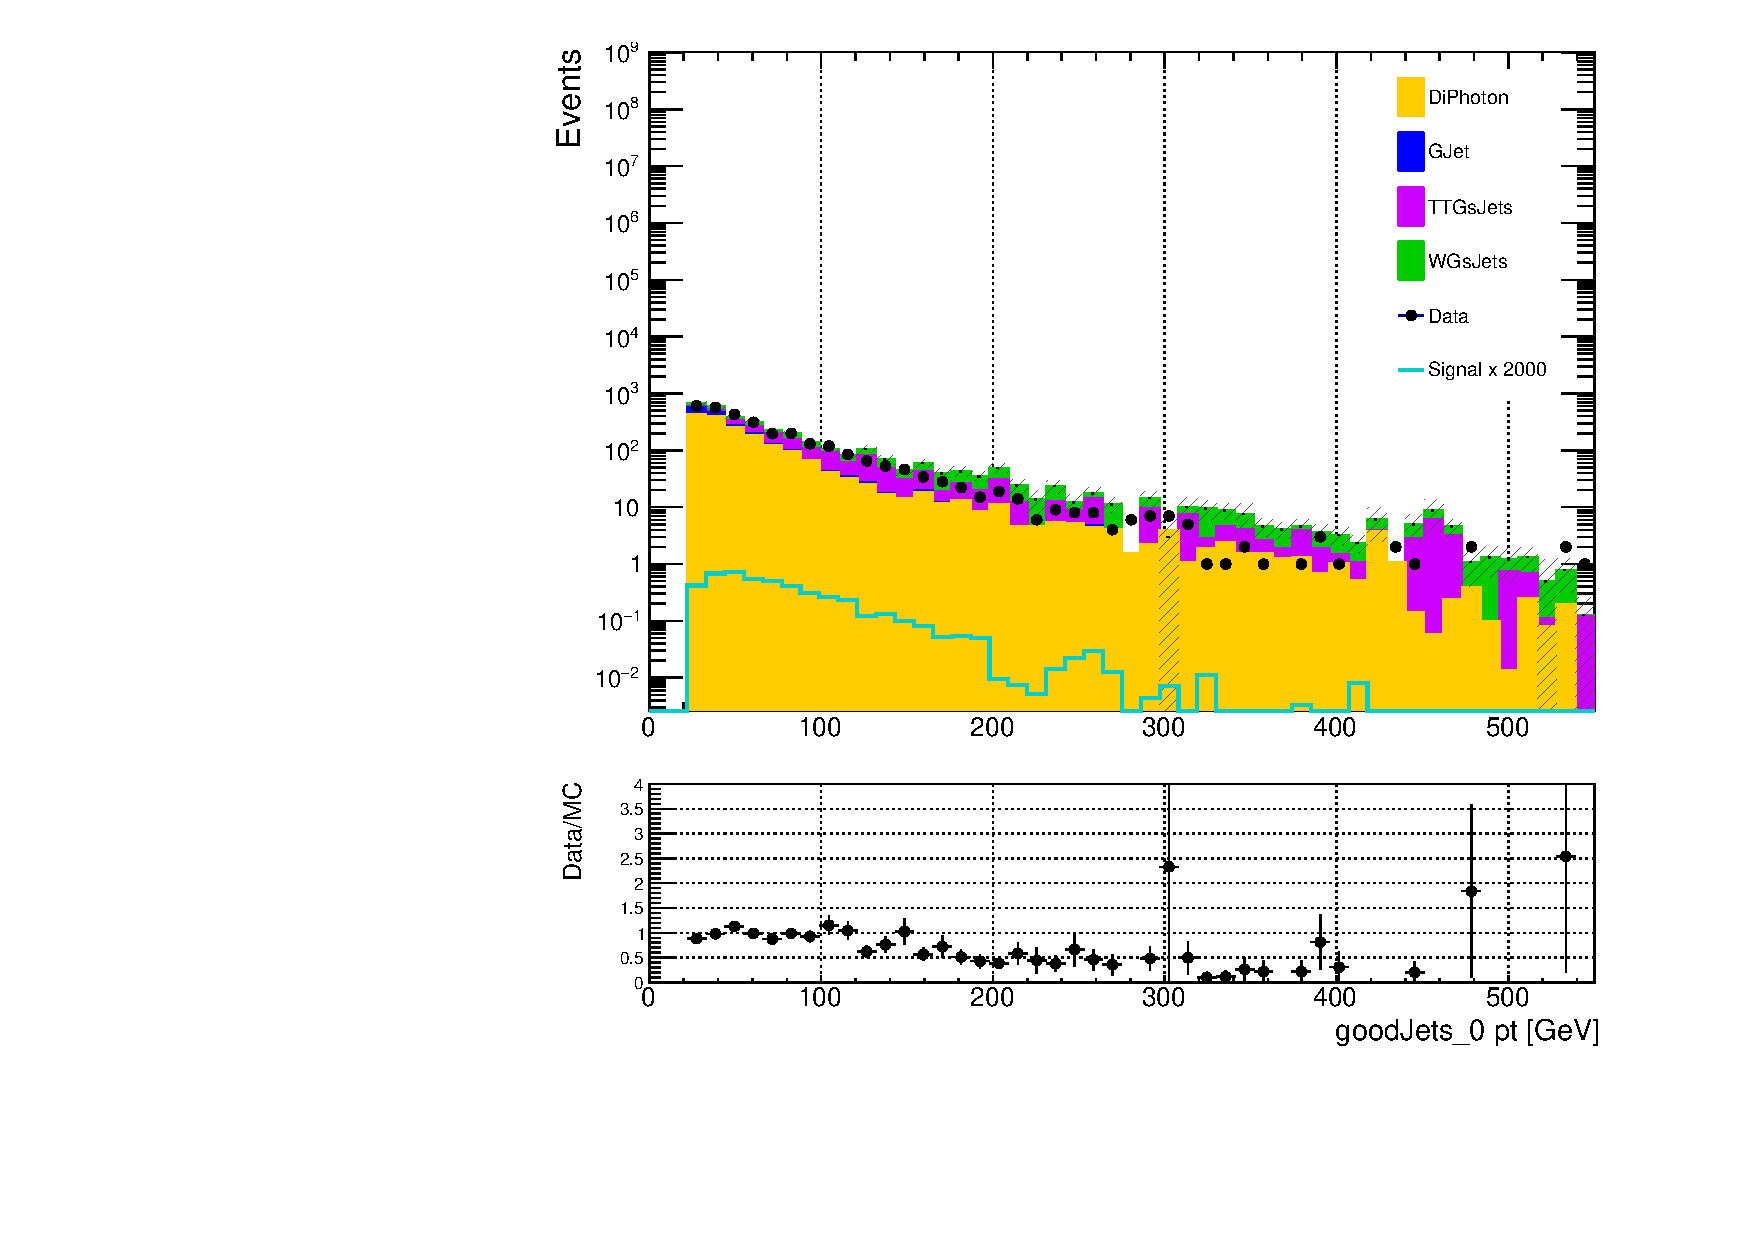
\includegraphics[width=0.45\textwidth]{Sections/HHWWgg/images/Semileptonic_Kinematic_Reweighting/Data_MC_WithKinWeights/goodJets_0_pt_log.pdf}\label{fig:Kin_Reweight_0_withKinWeights}}
    \caption{Leading jet \pt before and after kinematic reweighting (before any DNN evaluation), in the data sideband (100 $<$ $\mgg$ $<$ 115 or 135 $<$ $\mgg$ $<$ 180 GeV)}
    \label{fig:Kin_Reweight_0}
\end{figure} 

\begin{figure}[h!]
    \setcounter{subfigure}{0}
    \centering
    \subfloat[Before kinematic reweighting applied]{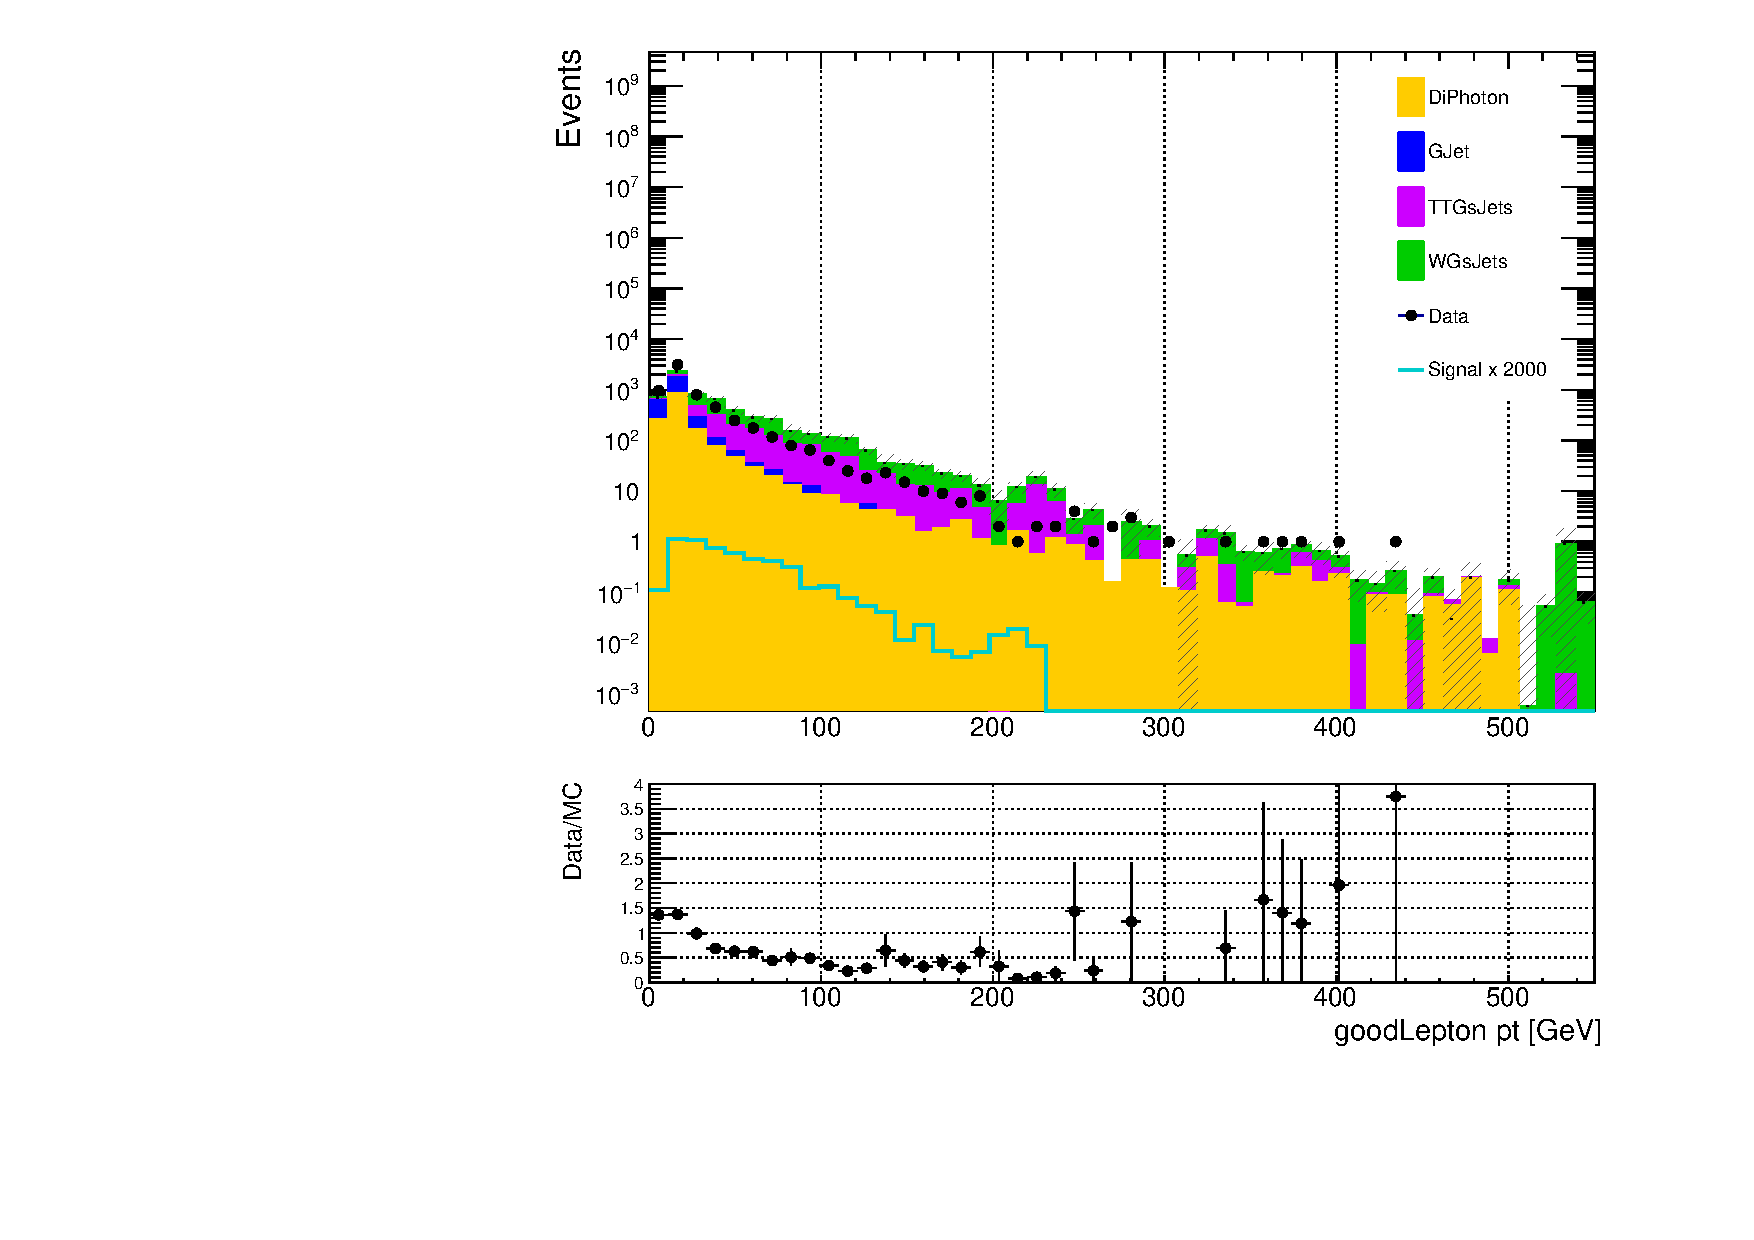
\includegraphics[width=0.45\textwidth]{Sections/HHWWgg/images/Semileptonic_Kinematic_Reweighting/Data_MC_WithoutKinWeights/goodLepton_pt_log.pdf}\label{fig:Kin_Reweight_1_withoutKinWeights}}
    \qquad
    \subfloat[After kinematic reweighting applied]{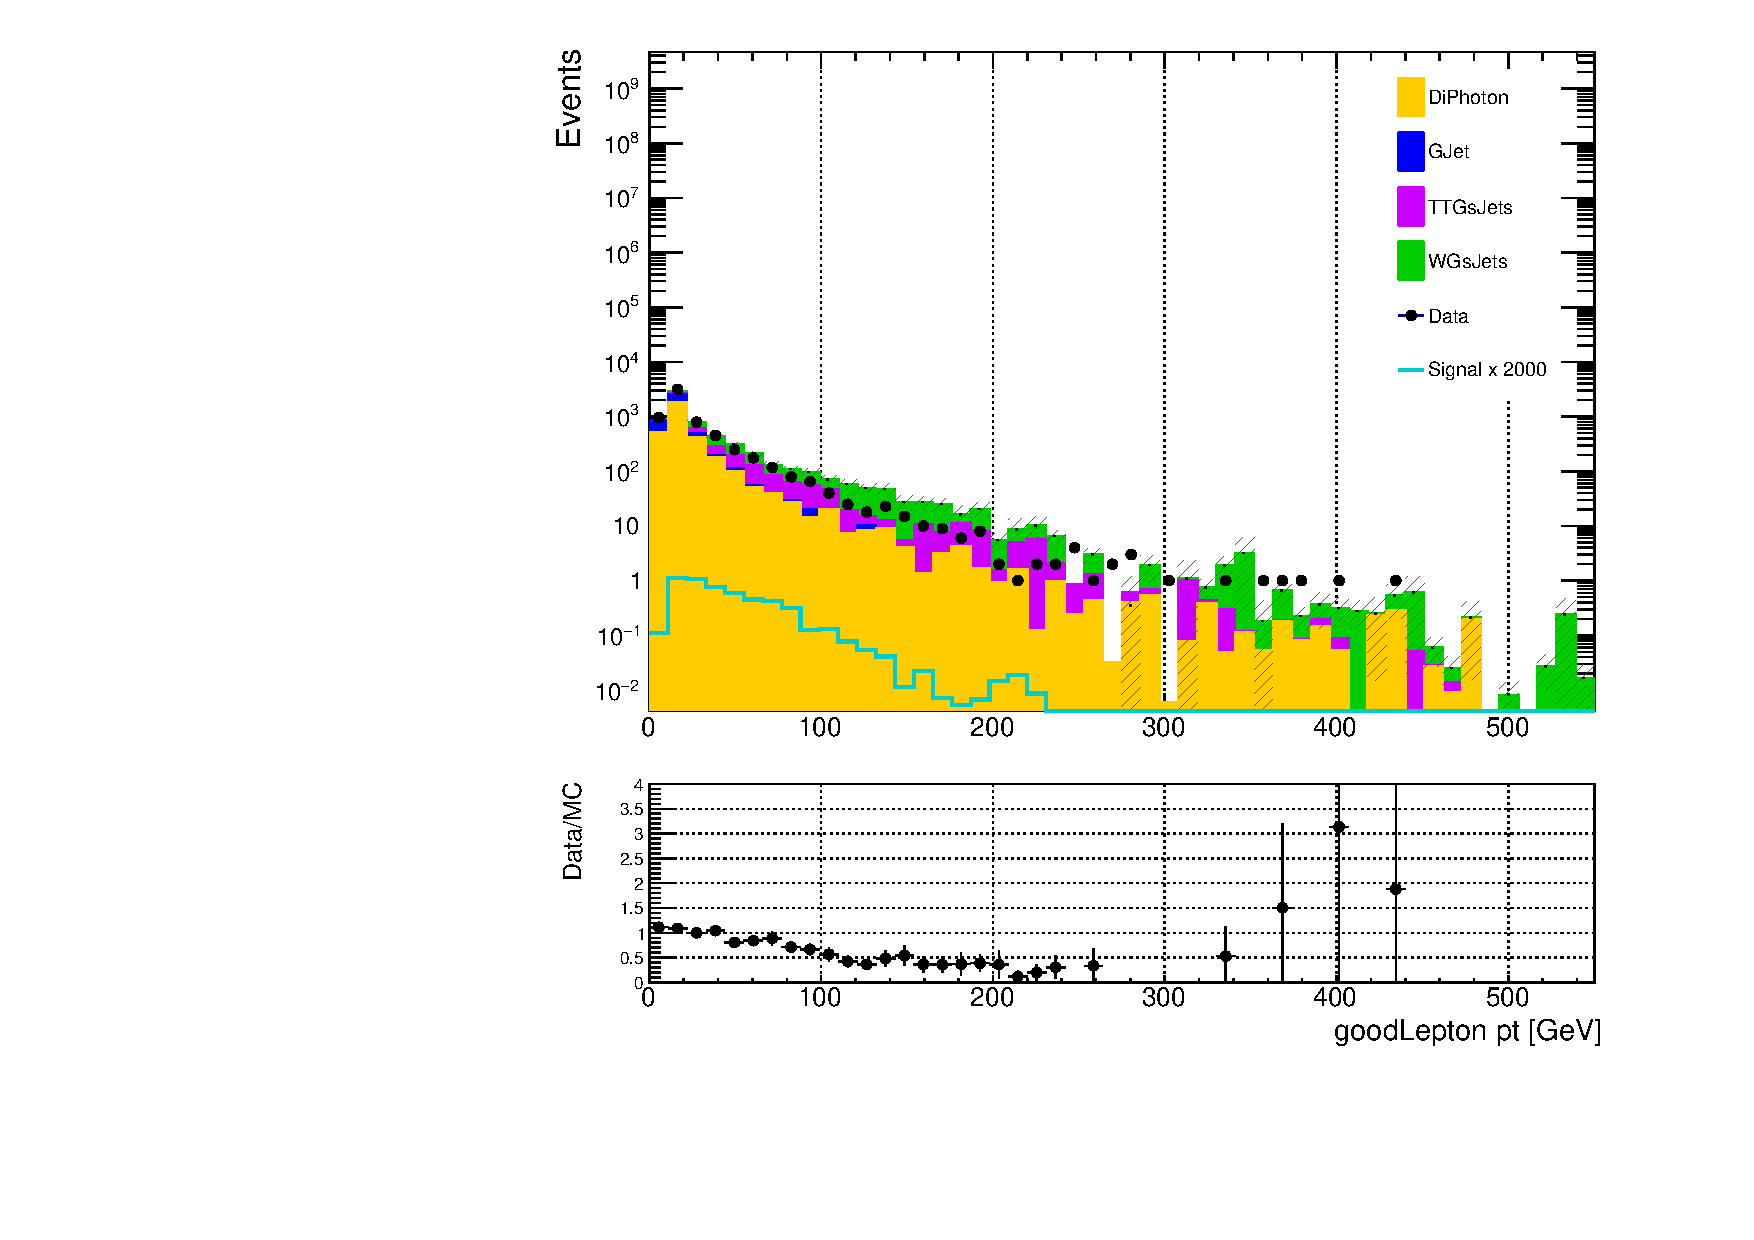
\includegraphics[width=0.45\textwidth]{Sections/HHWWgg/images/Semileptonic_Kinematic_Reweighting/Data_MC_WithKinWeights/goodLepton_pt_log.pdf}\label{fig:Kin_Reweight_1_withKinWeights}}
    \caption{Lepton \pt before and after kinematic reweighting (before any DNN evaluation), in the data sideband (100 $<$ $\mgg$ $<$ 115 or 135 $<$ $\mgg$ $<$ 180 GeV)}
    \label{fig:Kin_Reweight_2}
\end{figure} 

\begin{figure}[h!]
    \setcounter{subfigure}{0}
    \centering
    \subfloat[Before kinematic reweighting applied]{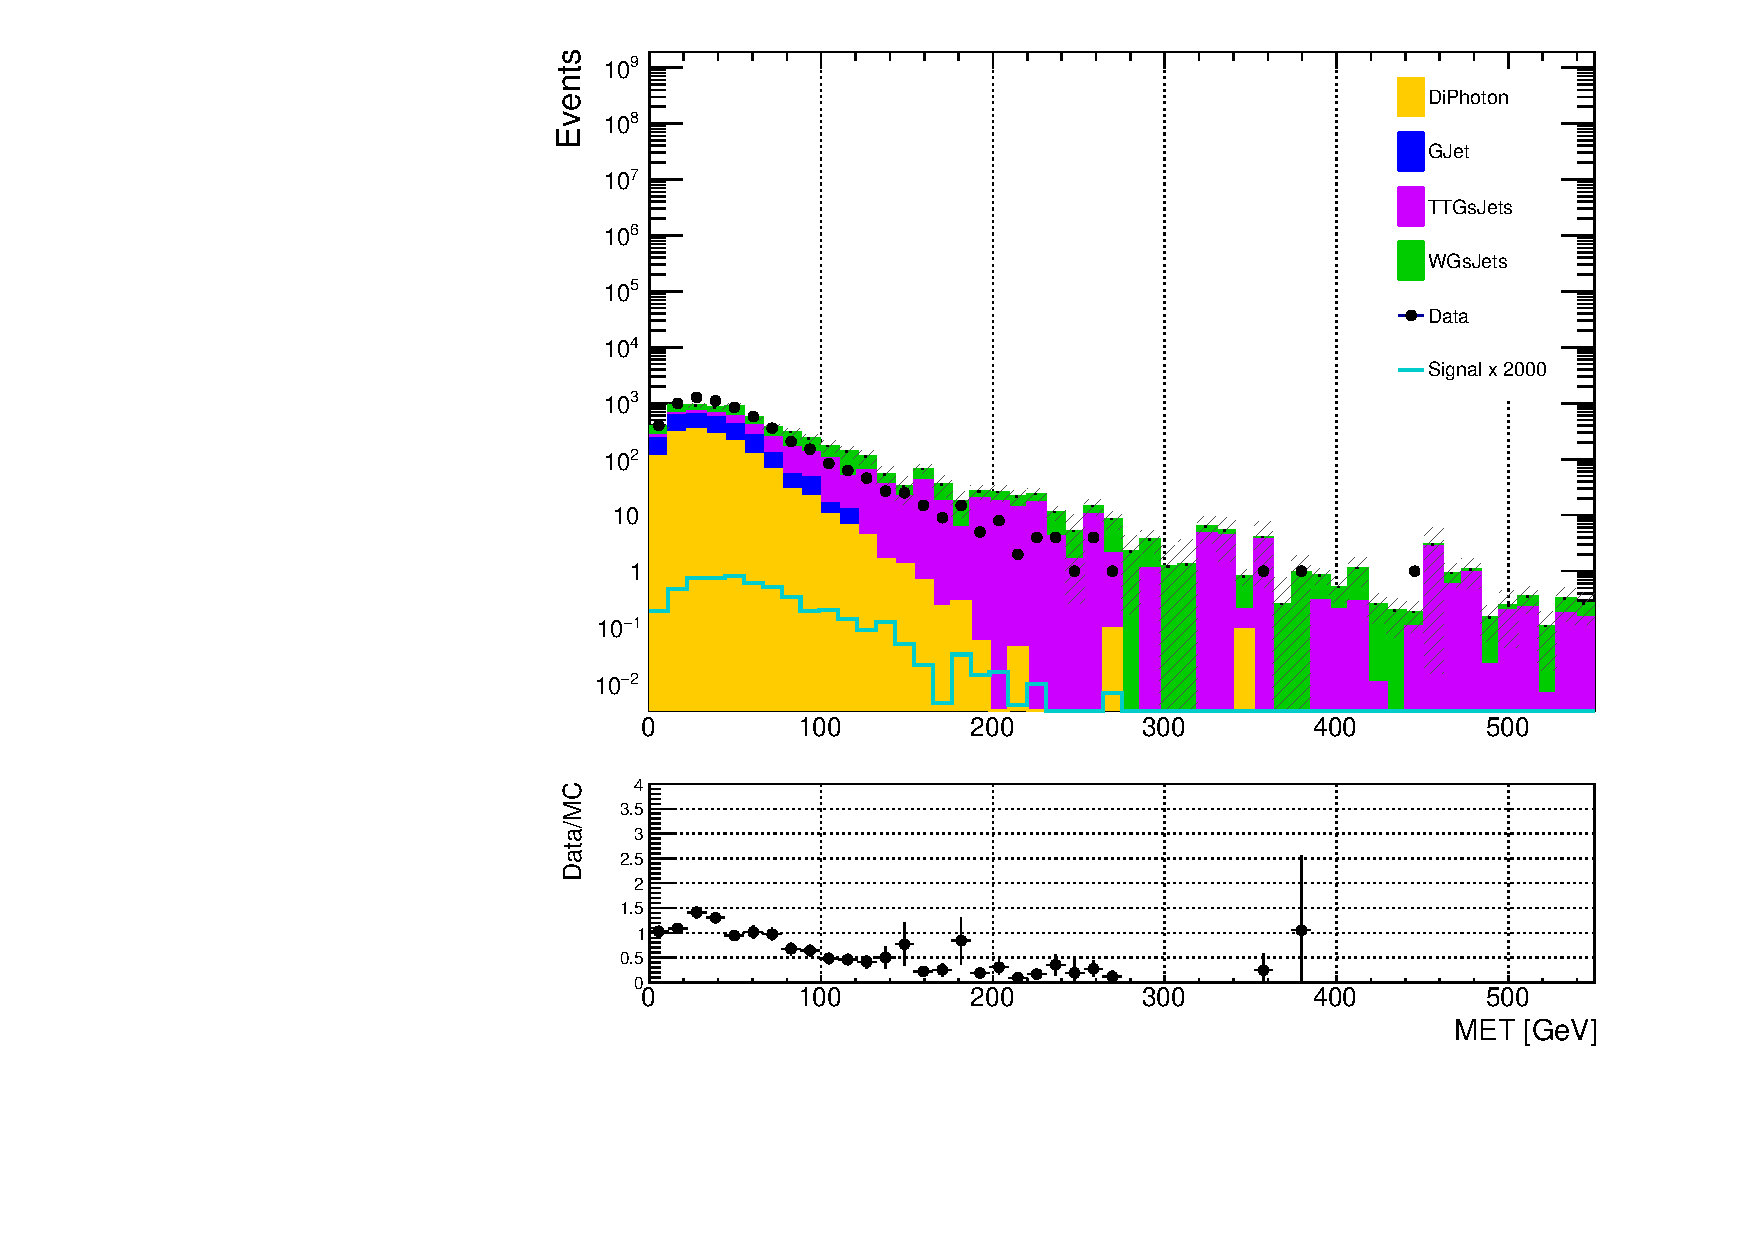
\includegraphics[width=0.45\textwidth]{Sections/HHWWgg/images/Semileptonic_Kinematic_Reweighting/Data_MC_WithoutKinWeights/MET_log.pdf}\label{fig:Kin_Reweight_2_withoutKinWeights}}
    \qquad
    \subfloat[After kinematic reweighting applied]{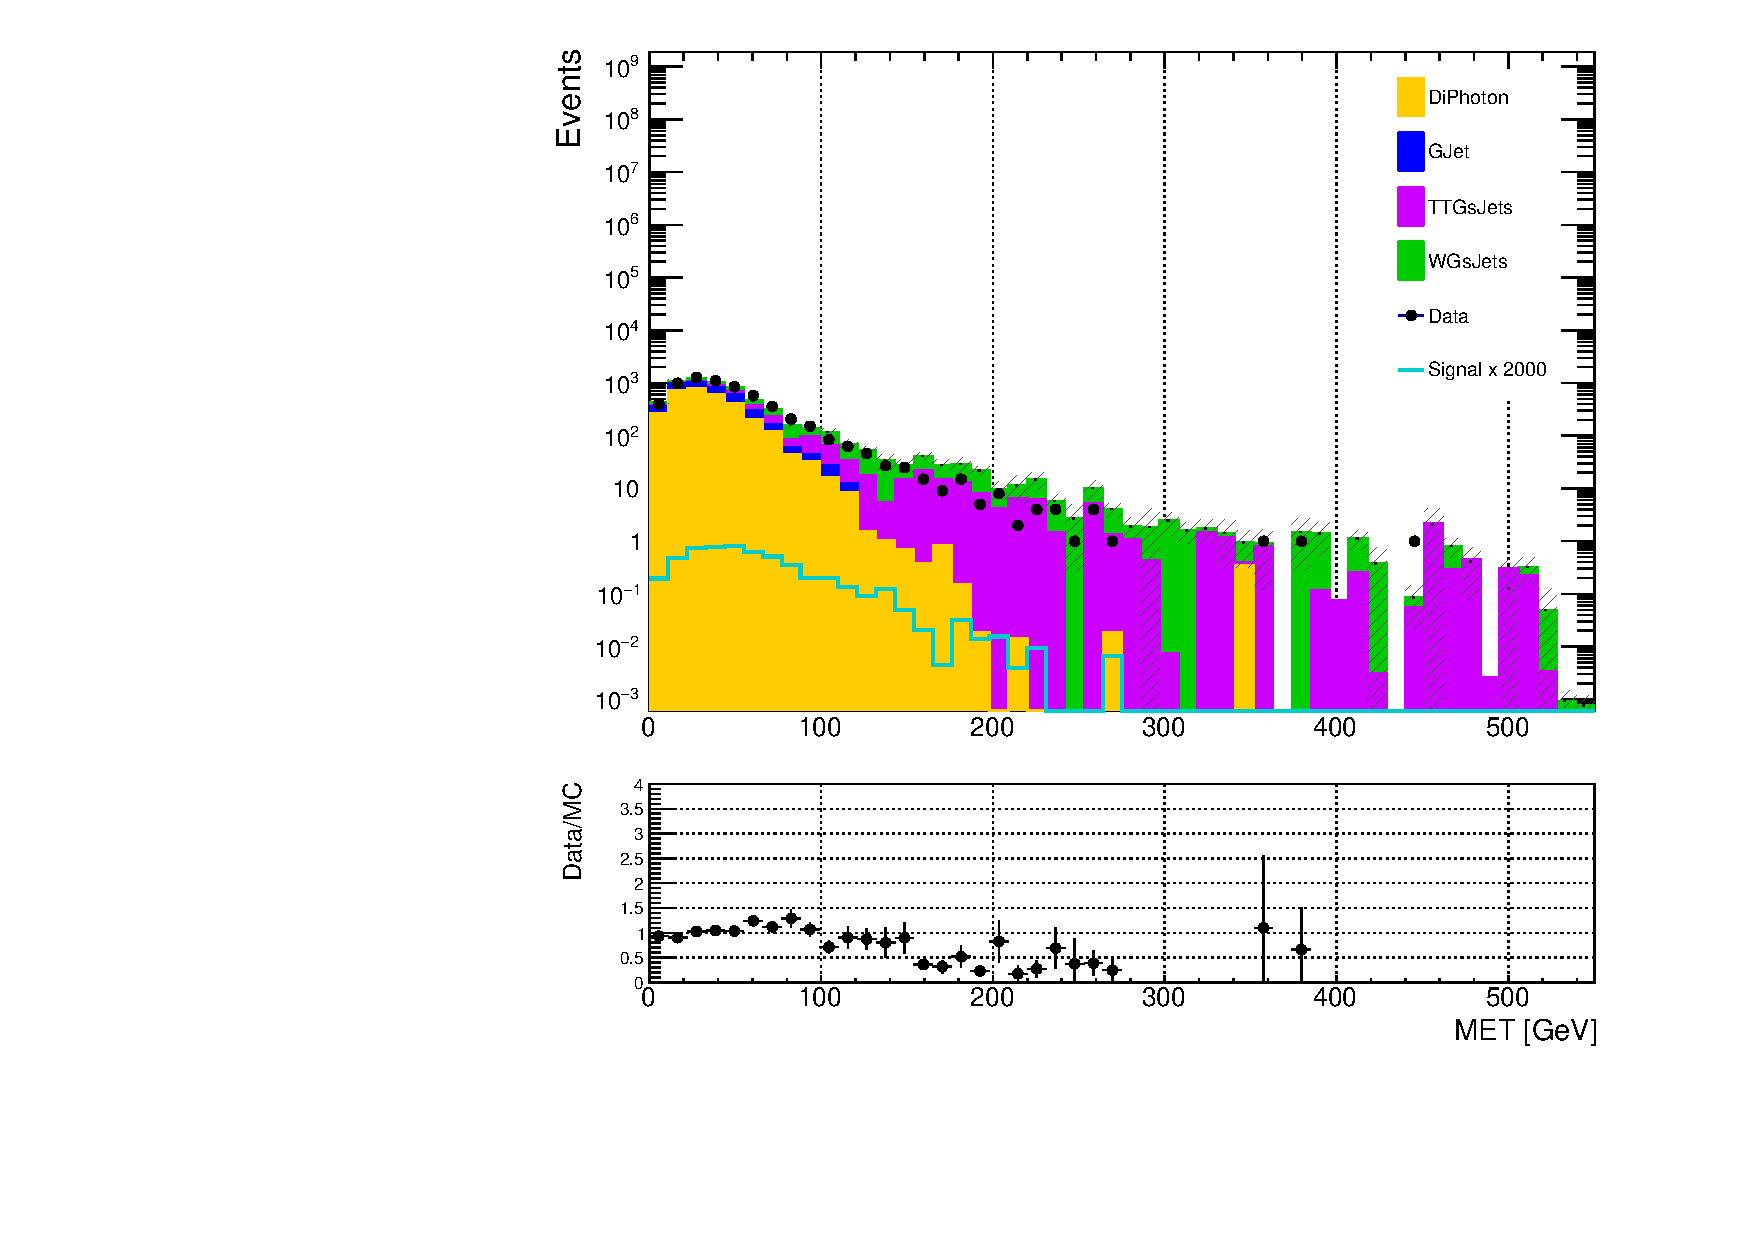
\includegraphics[width=0.45\textwidth]{Sections/HHWWgg/images/Semileptonic_Kinematic_Reweighting/Data_MC_WithKinWeights/MET_log.pdf}\label{fig:Kin_Reweight_2_withKinWeights}}
    \caption{MET before and after kinematic reweighting (before any DNN evaluation), in the data sideband (100 $<$ $\mgg$ $<$ 115 or 135 $<$ $\mgg$ $<$ 180 GeV)}
    \label{fig:Kin_Reweight_3}
\end{figure} 
  
\begin{figure}[h!]
    \setcounter{subfigure}{0}
    \centering
    \subfloat[Before kinematic reweighting applied]{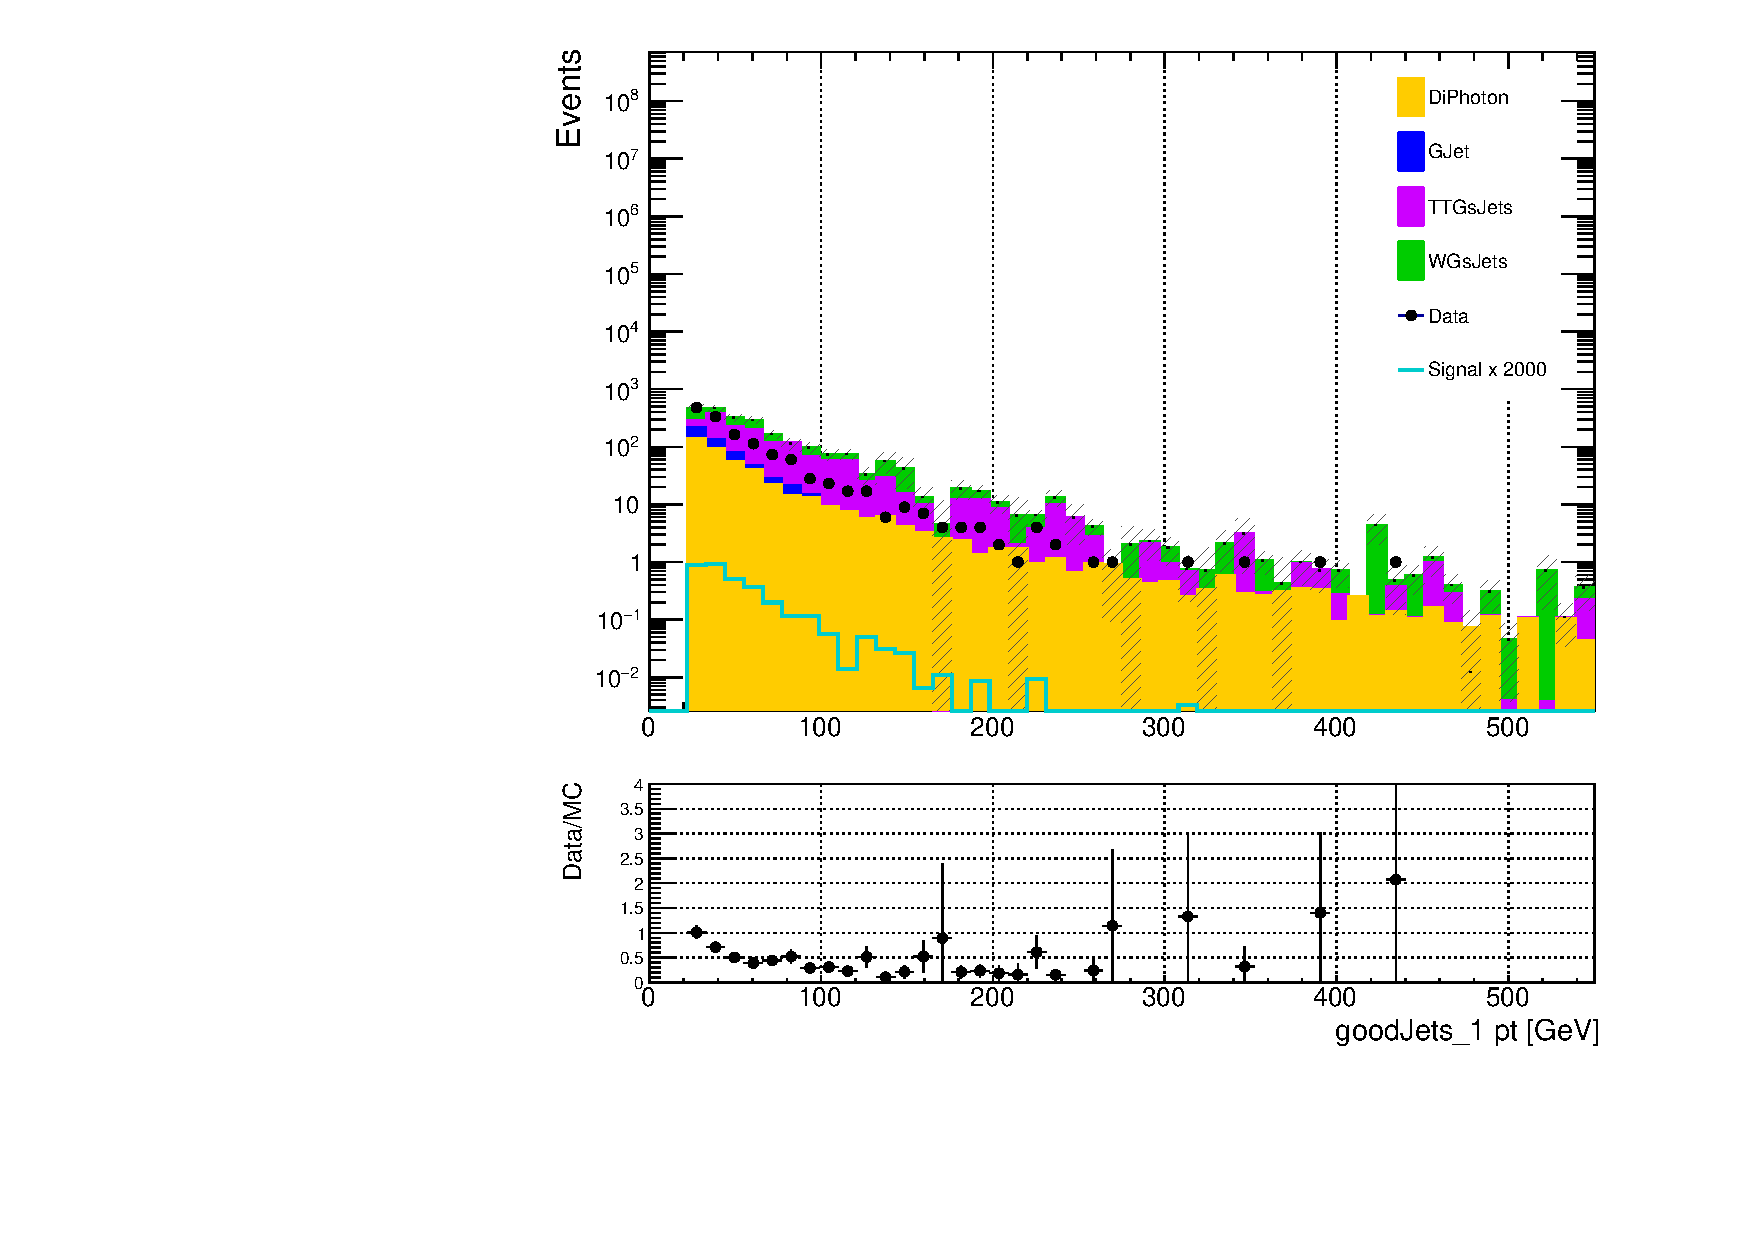
\includegraphics[width=0.45\textwidth]{Sections/HHWWgg/images/Semileptonic_Kinematic_Reweighting/Data_MC_WithoutKinWeights/goodJets_1_pt_log.pdf}\label{fig:Kin_Reweight_3_withoutKinWeights}}
    \qquad
    \subfloat[After kinematic reweighting applied]{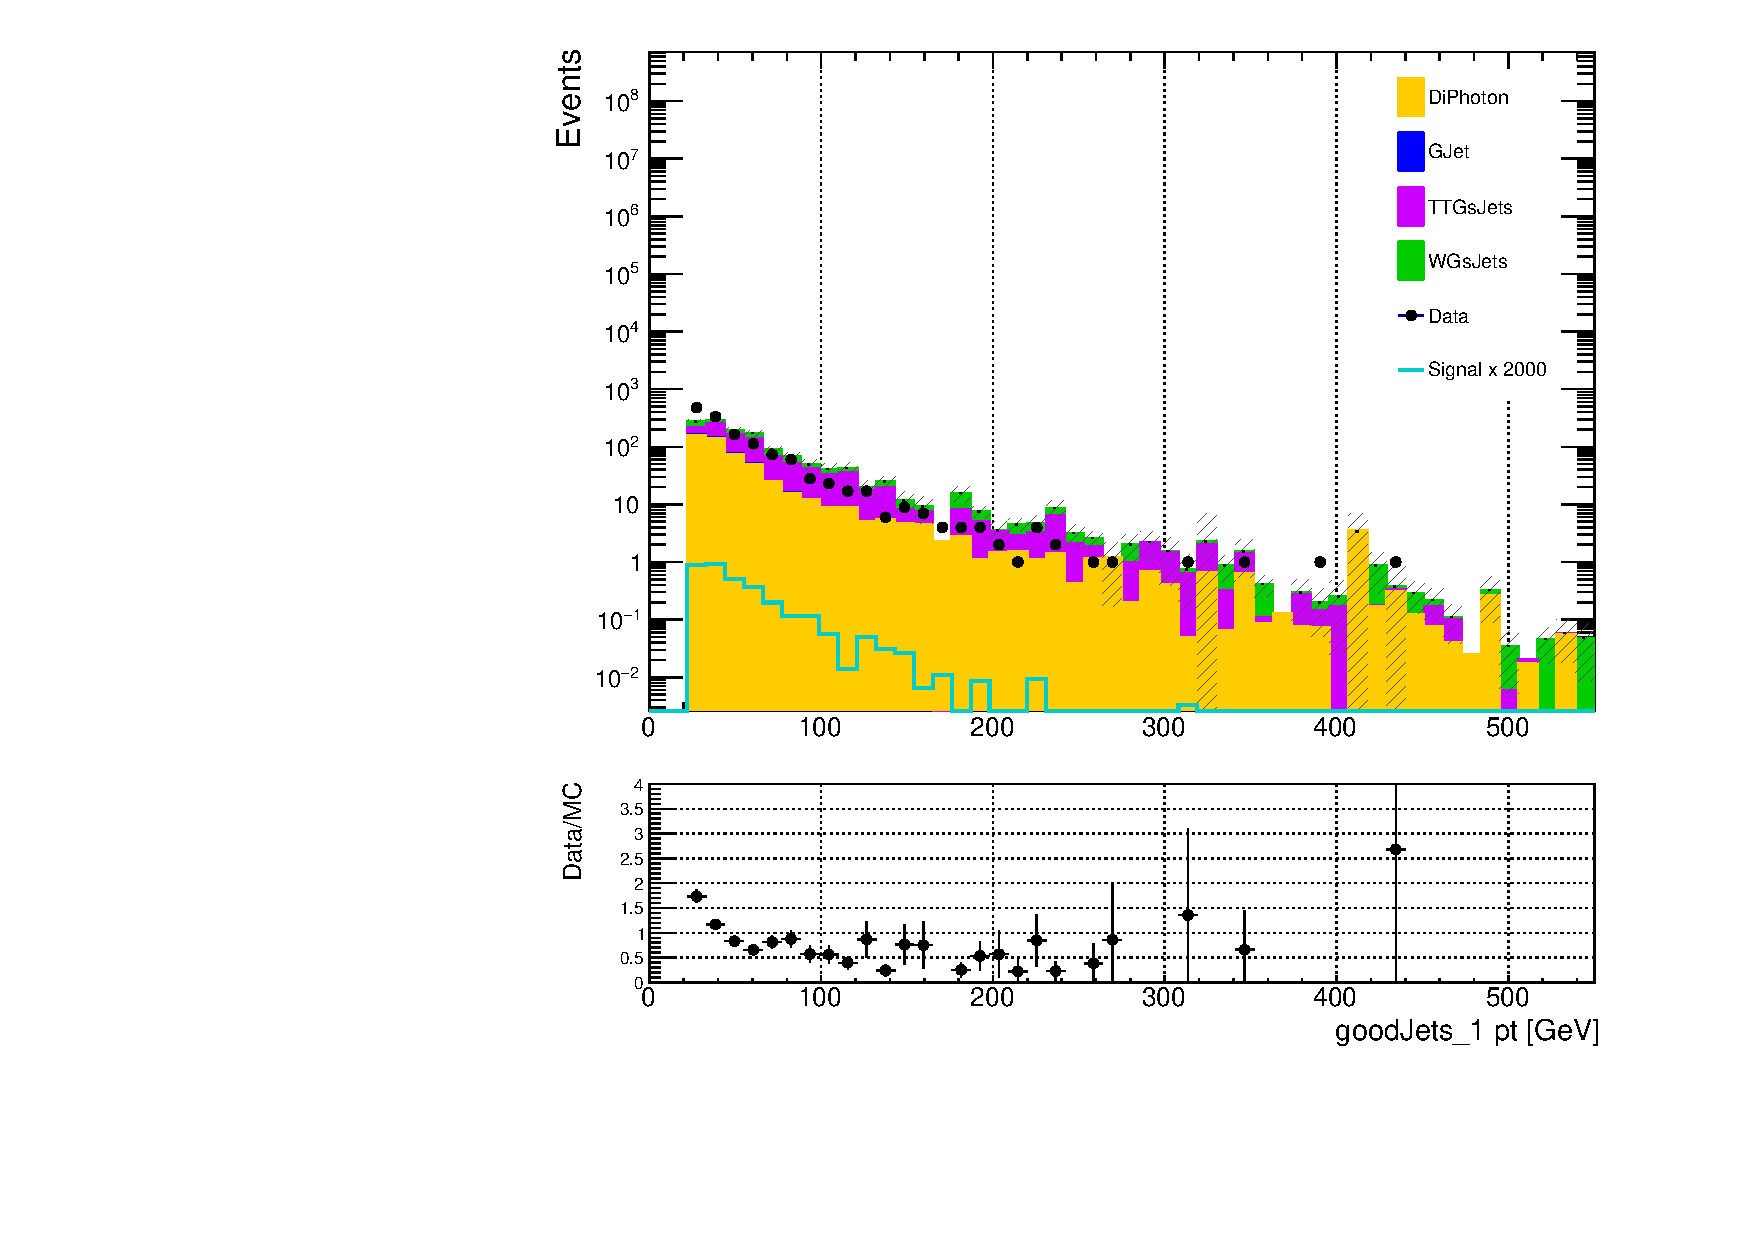
\includegraphics[width=0.45\textwidth]{Sections/HHWWgg/images/Semileptonic_Kinematic_Reweighting/Data_MC_WithKinWeights/goodJets_1_pt_log.pdf}\label{fig:Kin_Reweight_3_withKinWeights}}
    \caption{Subleading jet \pt before and after kinematic reweighting (before any DNN evaluation), in the data sideband (100 $<$ $\mgg$ $<$ 115 or 135 $<$ $\mgg$ $<$ 180 GeV)}
    \label{fig:Kin_Reweight_1}
\end{figure} 

\begin{figure}[h!]
    \setcounter{subfigure}{0}
    \centering
    \subfloat[Before kinematic reweighting applied]{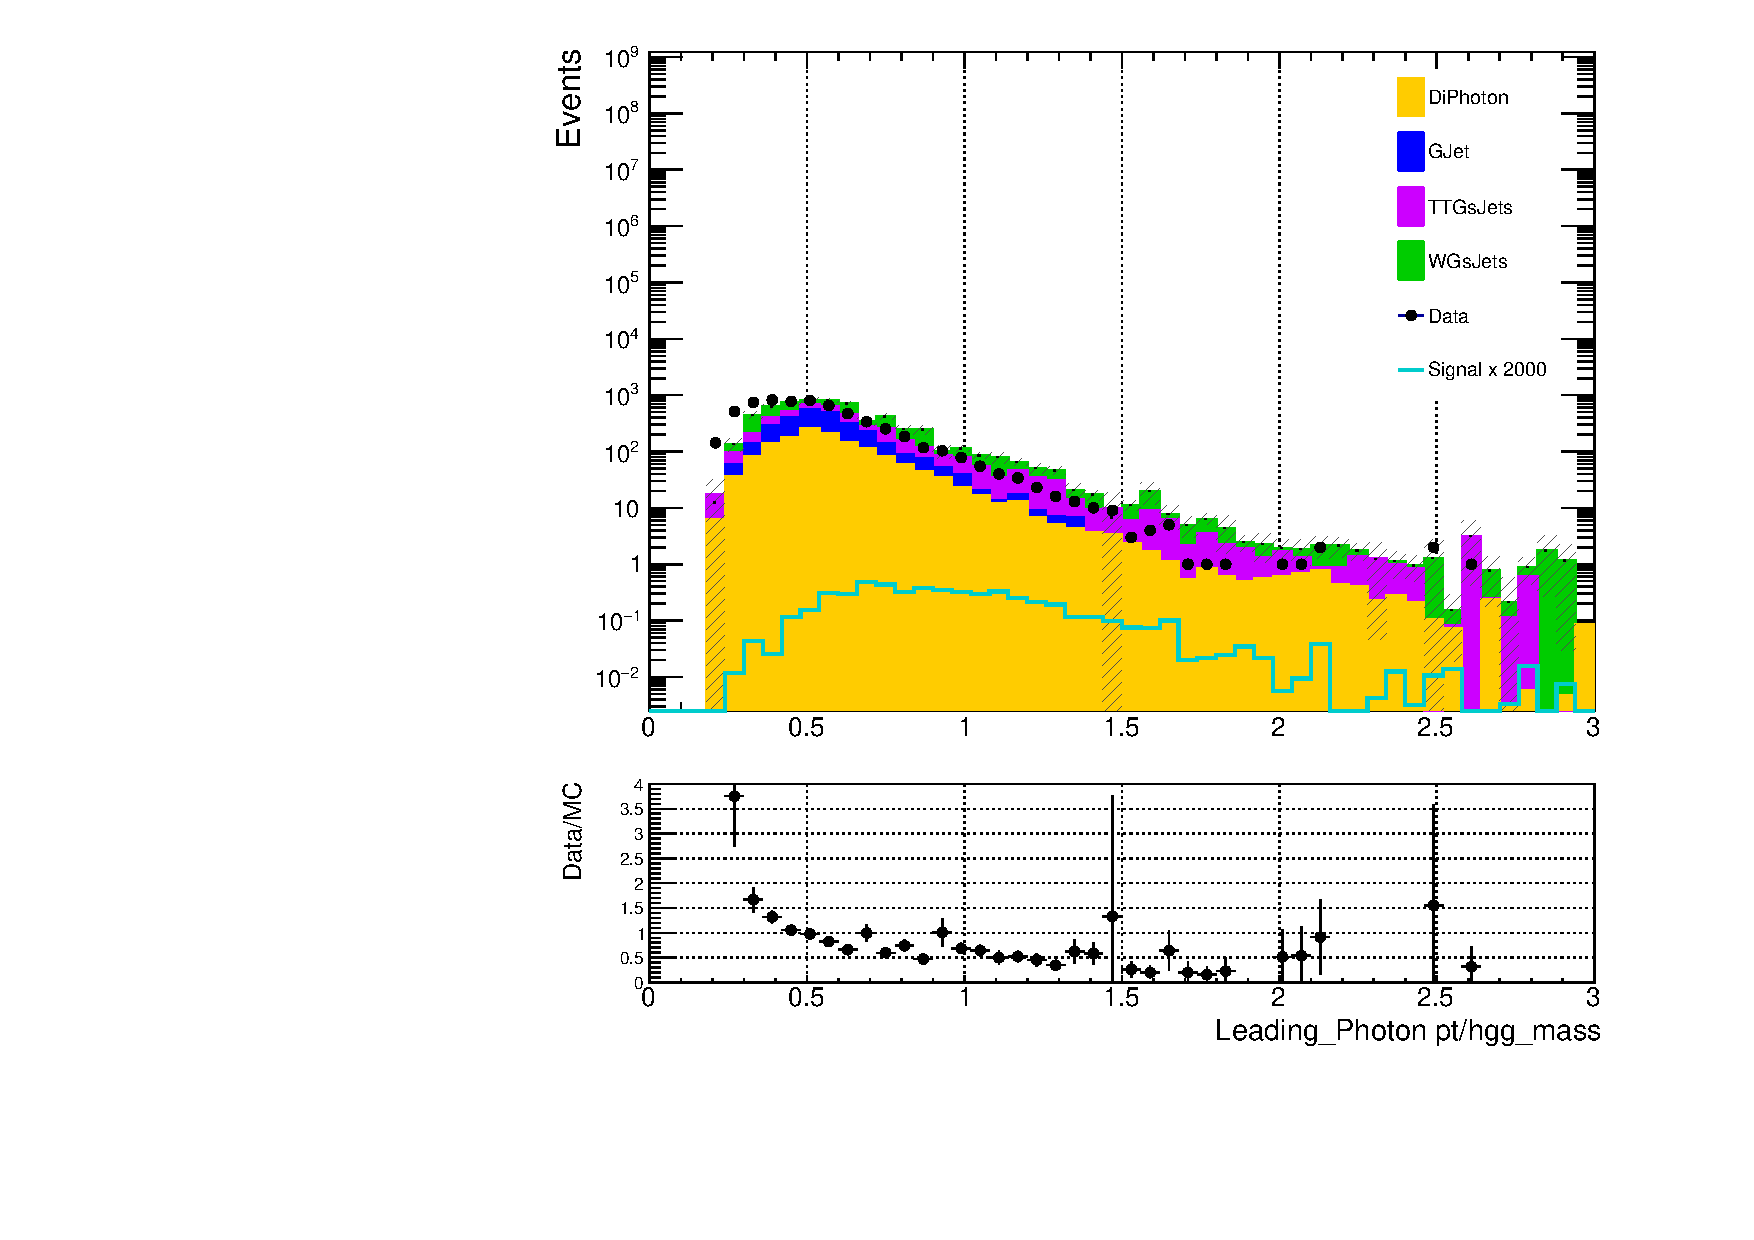
\includegraphics[width=0.45\textwidth]{Sections/HHWWgg/images/Semileptonic_Kinematic_Reweighting/Data_MC_WithoutKinWeights/Leading_Photon_pt_over_CMS_hgg_mass_log.pdf}\label{fig:Kin_Reweight_4_withoutKinWeights}}
    \qquad
    \subfloat[After kinematic reweighting applied]{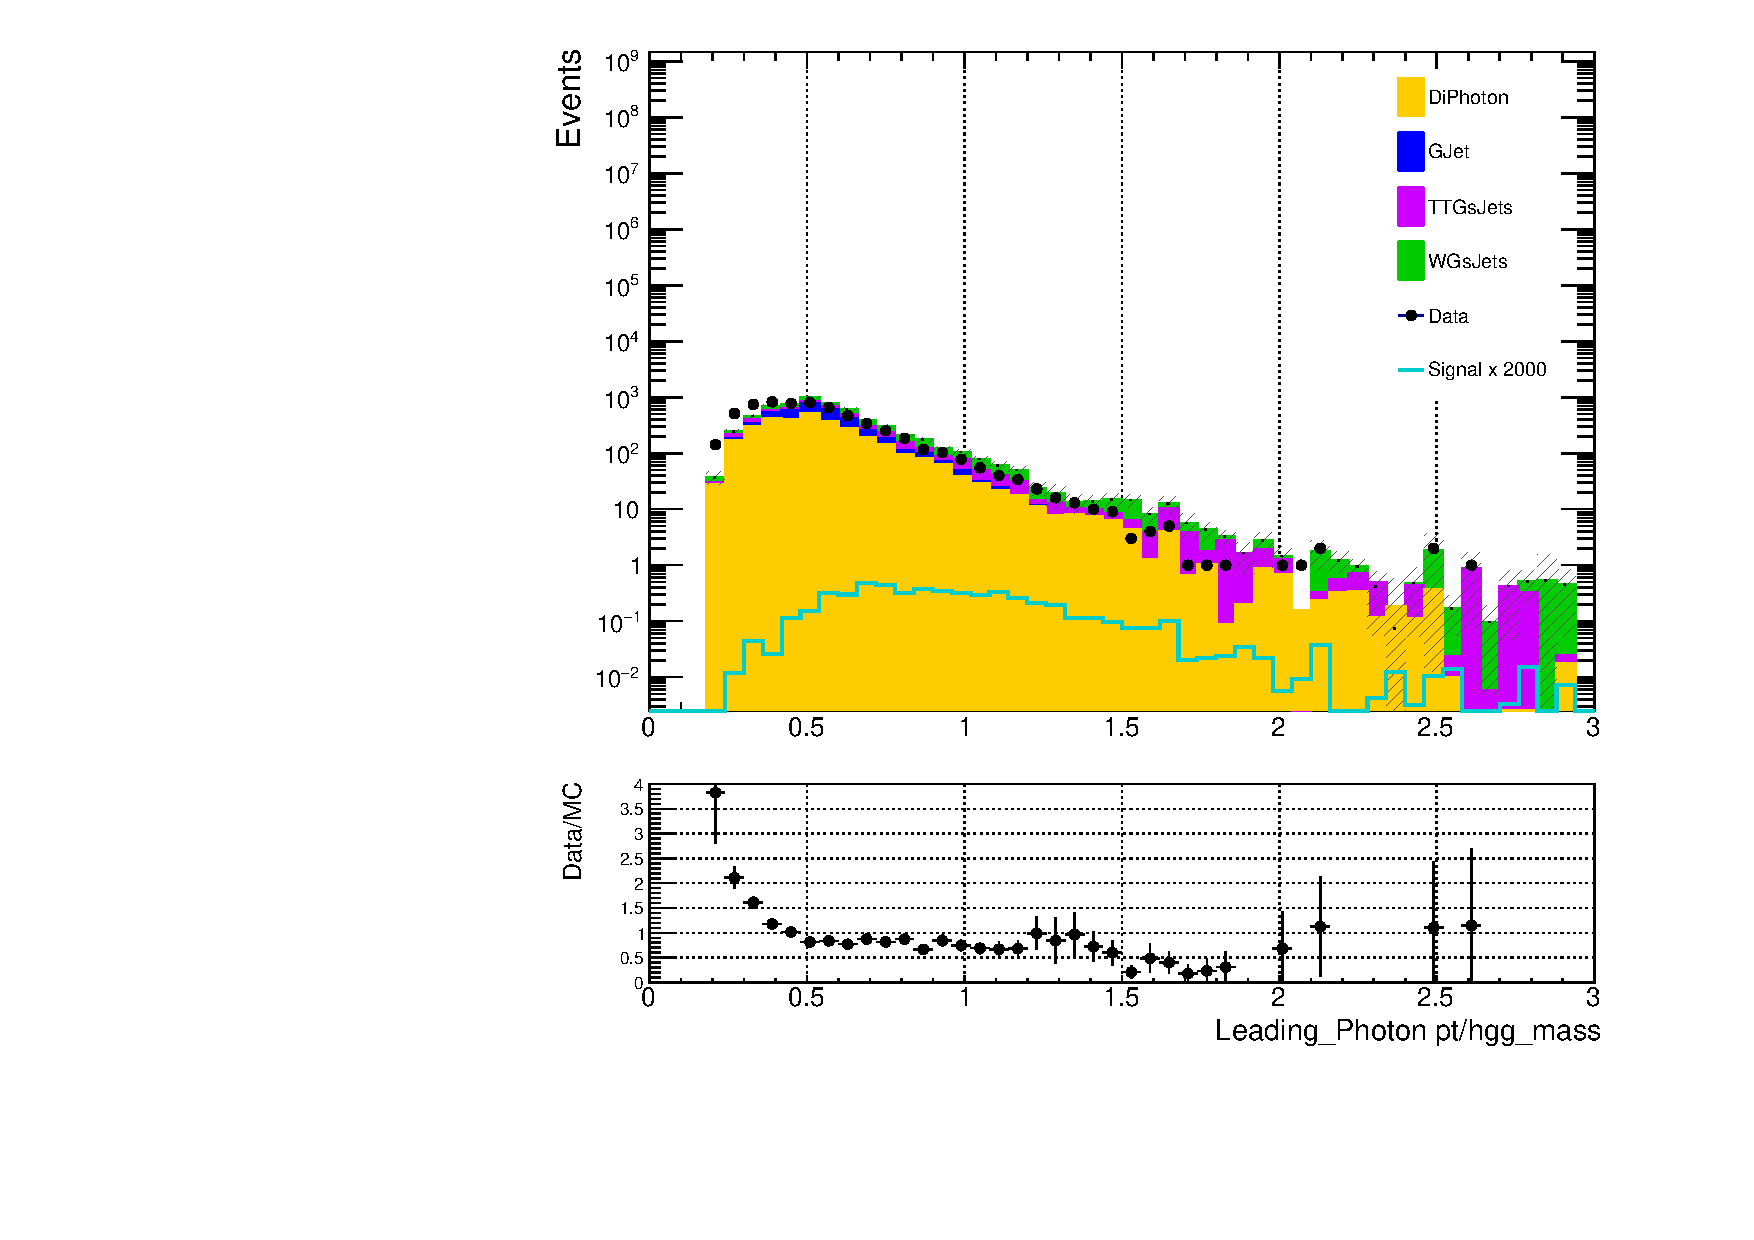
\includegraphics[width=0.45\textwidth]{Sections/HHWWgg/images/Semileptonic_Kinematic_Reweighting/Data_MC_WithKinWeights/Leading_Photon_pt_over_CMS_hgg_mass_log.pdf}\label{fig:Kin_Reweight_4_withKinWeights}}
    \caption{Leading photon \pt over \mgg before and after kinematic reweighting (before any DNN evaluation), in the data sideband (100 $<$ $\mgg$ $<$ 115 or 135 $<$ $\mgg$ $<$ 180 GeV)}
    \label{fig:Kin_Reweight_4}
\end{figure} 

\begin{figure}[h!]
    \setcounter{subfigure}{0}
    \centering
    \subfloat[Before kinematic reweighting applied]{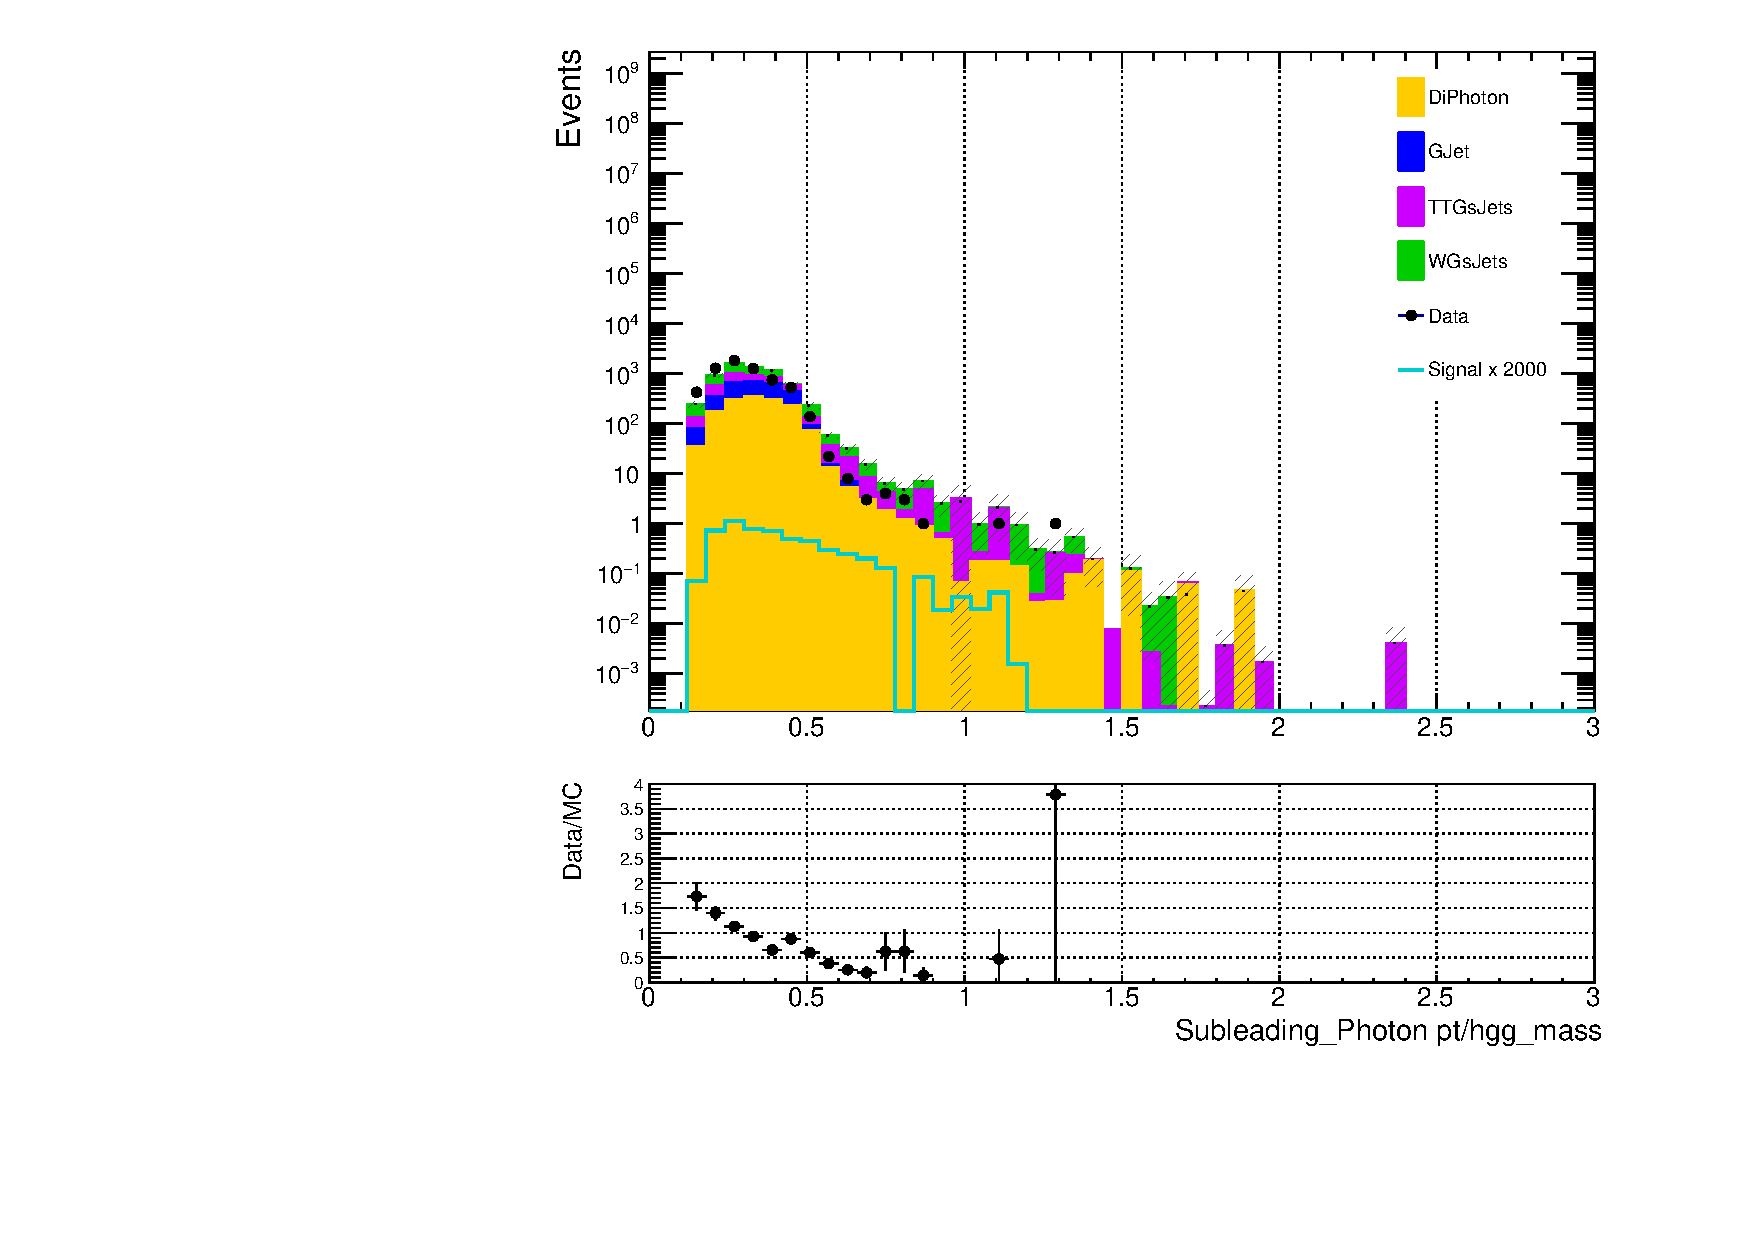
\includegraphics[width=0.45\textwidth]{Sections/HHWWgg/images/Semileptonic_Kinematic_Reweighting/Data_MC_WithoutKinWeights/Subleading_Photon_pt_over_CMS_hgg_mass_log.pdf}\label{fig:Kin_Reweight_5_withoutKinWeights}}
    \qquad
    \subfloat[After kinematic reweighting applied]{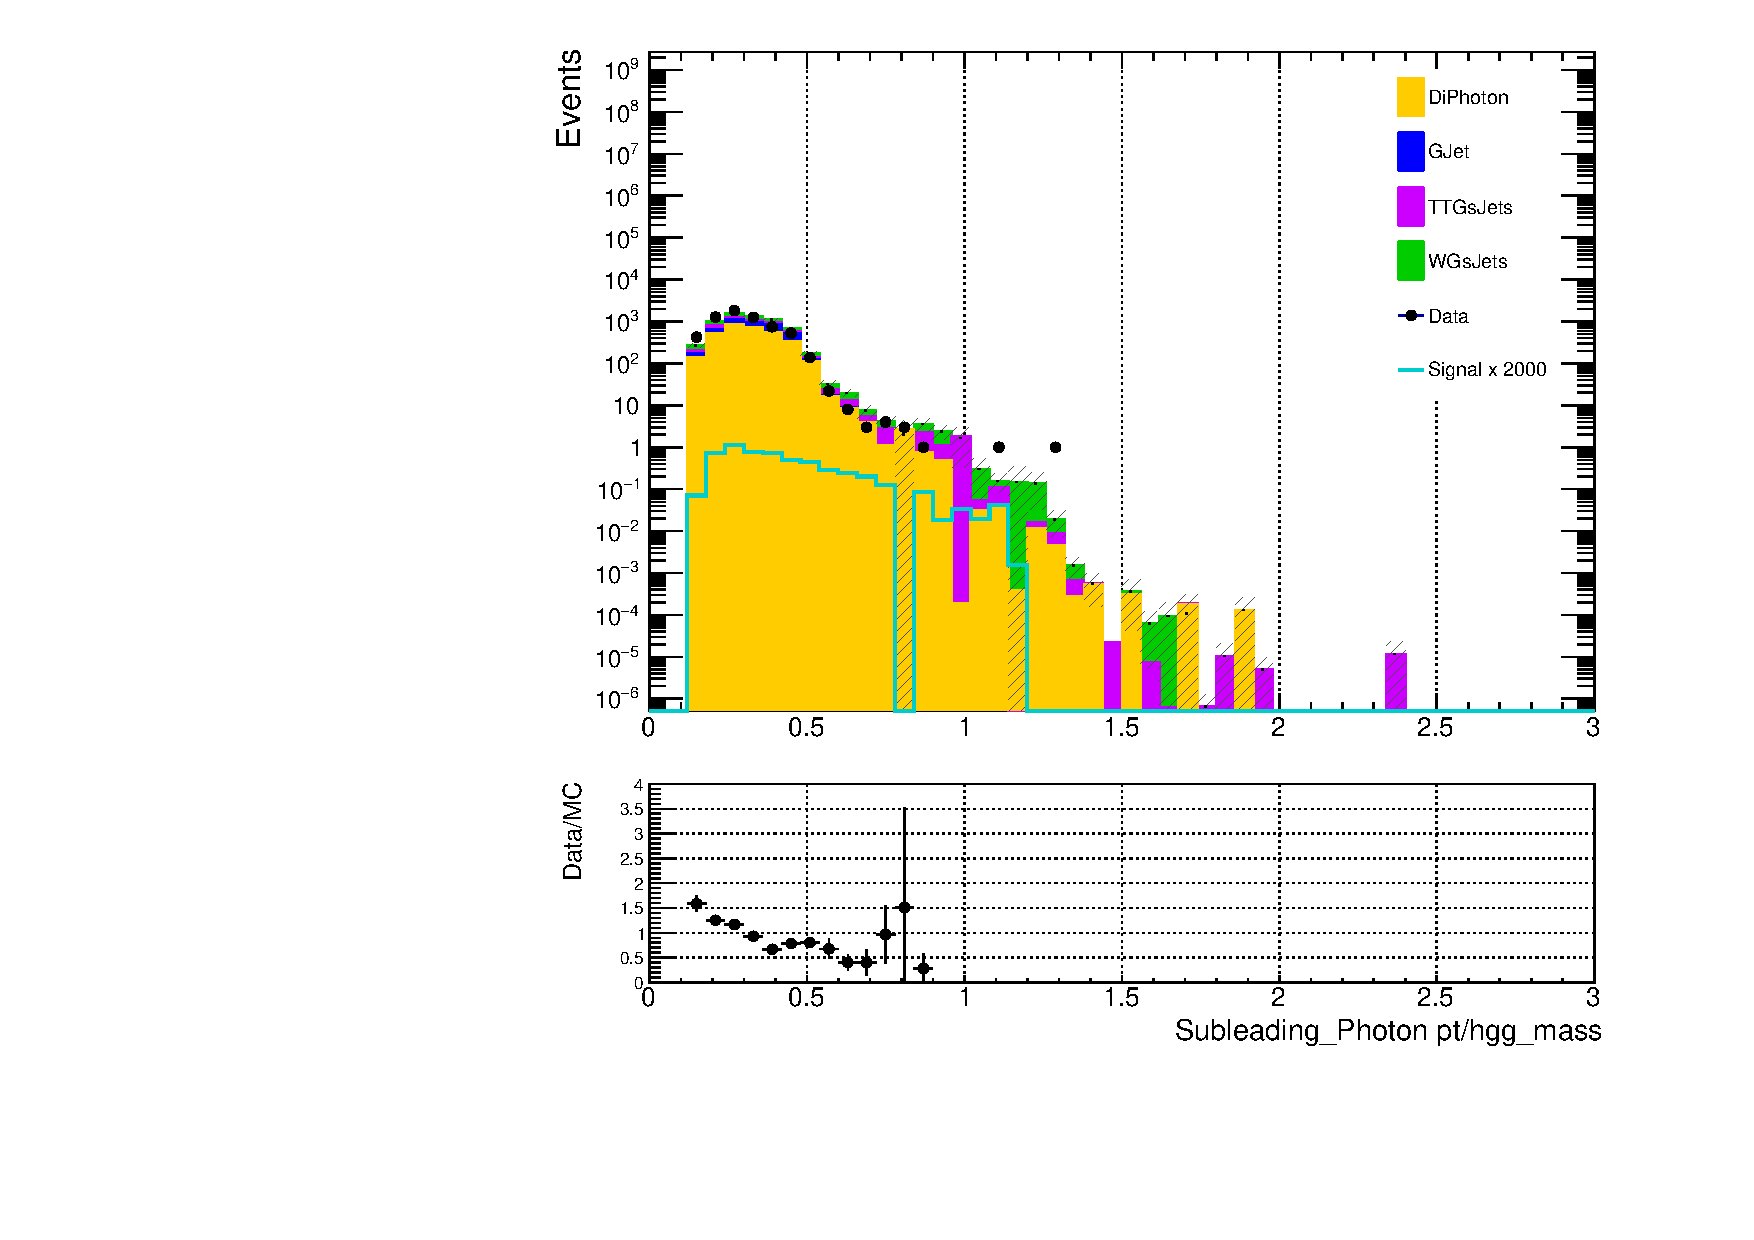
\includegraphics[width=0.45\textwidth]{Sections/HHWWgg/images/Semileptonic_Kinematic_Reweighting/Data_MC_WithKinWeights/Subleading_Photon_pt_over_CMS_hgg_mass_log.pdf}\label{fig:Kin_Reweight_5_withKinWeights}}
    \caption{Subleading photon \pt over \mgg before and after kinematic reweighting (before any DNN evaluation), in the data sideband (100 $<$ $\mgg$ $<$ 115 or 135 $<$ $\mgg$ $<$ 180 GeV)}
    \label{fig:Kin_Reweight_5}
\end{figure} 

\clearpage 

The MultiClass DNN outputs three DNN scores, each with a range 0-1 and corresponding to the likelihood that an event falls into each of the three classes, which sum to one. This means that if an event has a high 
HH class DNN score, the sum of the H and continuum background DNN scores must be small. Because of this constraint, only the output HH class DNN score is used in the analysis for categorization as 
it has a known correlation to the output H and continuum background DNN scores. 

The DNN training results in the ROC (Receiver operating curve) shown in Figure \ref{fig:ROC_HH}, and normalized DNN scores for the three classes shown in Figure \ref{fig:SL_DNN_overfitting_check}.

A possible way to improve this analysis in the future would be to make use of the H and continuum background DNN scores, for instance in order to define control regions with high H and continuum background but low HH yields. These could potentially be included in the simultaneous fit to data in order to decrease the statistical uncertainty, and improve the modelling of the single Higgs templates in the signal region.  

Due to the non-linearity of deep neural network models, understanding the relative importance of the input features is non-trivial. In this analysis,
we evaluate the relative importance by evaluating Shapley values \cite{shapley_values} for each feature. The Shapley value is the average of the marginal
contribution of a feature's value to the prediction, across all possible coalitions of features. Specifically, it is calculated by taking the difference in the
value of the prediction with and without a given feature (the marginal contribution). This is repeated for all possible combinations of the other input features and
the average value of the marginal contributions is taken as the Shapely value. It is important to note that the Shapley value is the average contribution of a feature
value to the prediction in the different coalitions of features and not the difference in prediction with and without the feature in the model. 
It is also worth noting that coalitions of features can be formed without the complete list of input features. When this happens, in order to
evaluate the network the missing feature(s) value is randomised in order to obtain a prediction. The relative importance of the input features can be found in
Figure \ref{fig:SLfeatureranking_HH}, for the HH class DNN score. The variables are
ranked from highest to lowest in order of their discriminatory power per class. The leading importance variables all correspond to quantities from the final state topology of the semi-leptonic WW$\gamma\gamma$ process, namely two photons, one lepton, two jets and a neutrino.

\begin{figure}[H]
  \setcounter{subfigure}{0}
  \centering
  \subfloat[All Shapley scores]{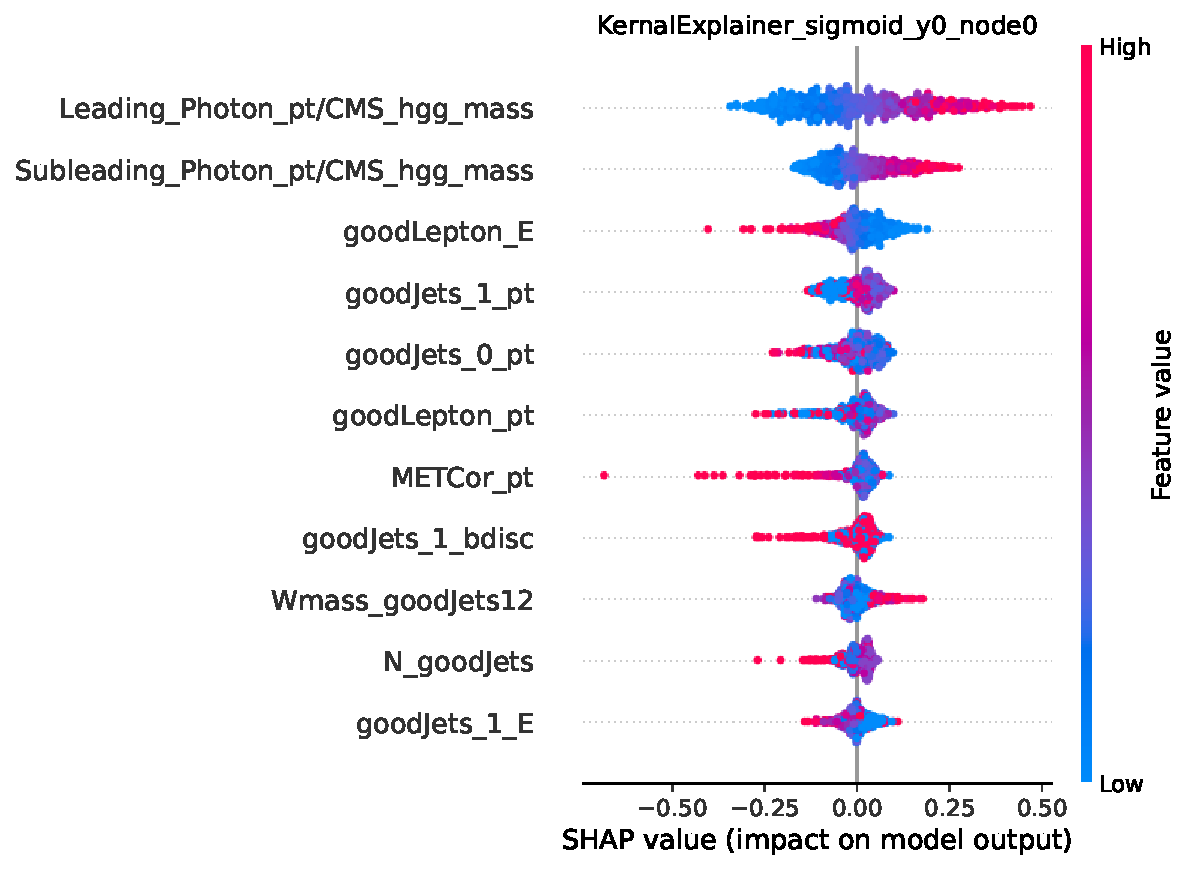
\includegraphics[width=0.45\textwidth]{Sections/HHWWgg/images/DNN/KernalExplainer_sigmoid_y0_node0.pdf}}
  %\qquad
  \subfloat[Average Shapley score magnitudes]{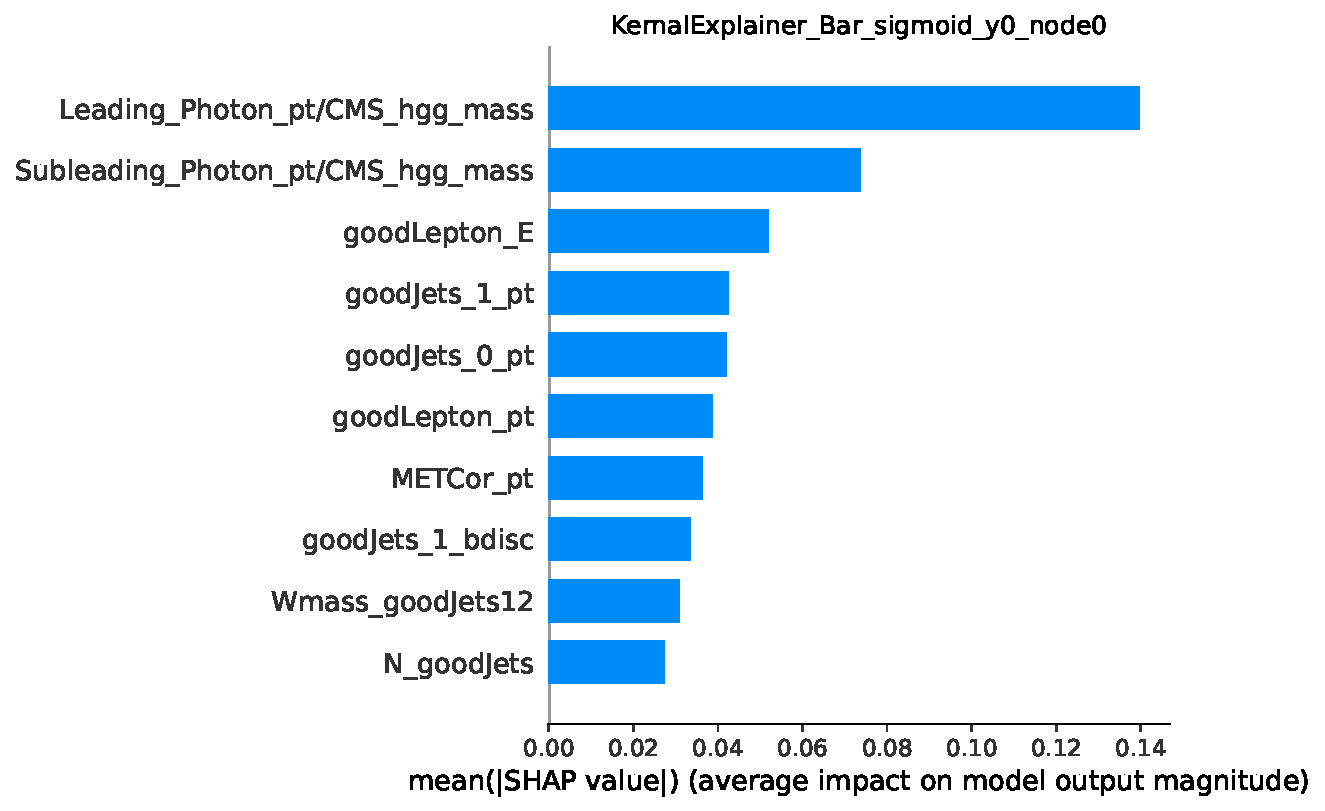
\includegraphics[width=0.45\textwidth]{Sections/HHWWgg/images/DNN/KernalExplainer_Bar_sigmoid_y0_node0.pdf}}
  \caption{Semi-leptonic channel DNN input feature ranking according to Shapely values in the HH class}
  \label{fig:SLfeatureranking_HH}
\end{figure} 

\begin{figure}[H]
  \setlength{\unitlength}{1mm}
  \begin{center}
    \mbox{\includegraphics*[height=100mm]{Sections/HHWWgg/images/DNN/MultiClass_ROC_class_HH.pdf}
    }
  \end{center}
  \caption{Semi-Leptonic DNN ROC curve for training and test data: HH Class}
  \label{fig:ROC_HH}
\end{figure}

\begin{figure}[H]
  \setlength{\unitlength}{1mm}
  \begin{center}
    \mbox{\includegraphics*[height=100mm]{Sections/HHWWgg/images/DNN/overfitting_plot_HH_Non-Categorised.pdf}
    }
  \end{center}
  \caption{Normalized HH DNN score distributions for the three semileptonic DNN nodes, shown for training and test events.}
  \label{fig:SL_DNN_overfitting_check}
\end{figure}

% Data/MC after training:

% A single sideband weight is extracted and applied in order to compare the data and MC shapes. 

% The sideband weight is obtained and shapre comparison performed
% in the follow way: MC is scaled to the ratio of data / MC integrals
% in the sidebands, 

% of the di-photon mass in the data sidebands with and without this sideband weight value of 1.140 is shown in 
% Figure \ref{fig:DNNSidebands_withAndWithoutSidebandScale}.

Events with a DNN score less than 0.1 are removed and not used for categorization, nor in any background or signal modelling, as this region is largely background dominant. 

In order to qualitatively understand the level of optimization of the DNN in identifying data events with MC, the data / MC ratio comparison of events with a DNN score greater than 0.1 are shown for the leading importance input variables in Figures \ref{fig:SLDNNFeaturecontrolplots-1} and \ref{fig:SLDNNFeaturecontrolplots-2}. It should be noted 
that any disagreement between data and MC will lead to a sub-optimal network, but will not introduce any bias in the final result extraction, as MC is only used for selection and categorization optimization. 

% The data-MC ratio of all remaining input variables can be found in Appendix \ref{sec:DNN-Input-Variables}.

Table \ref{tab:SL_DNN_Background_yields} shows the post-selection yields, including a selection on the output DNN score of $>$ 0.1, for all of the simulated samples
used in this analysis, both the absolute number and the corresponding yield accounting for proper MC scaling.

The correlation plot of all input features can also be found in Figure \ref{fig:inputvarcorrelation} and is used to check if any correlations are present between input training variables. In particular it can 
be seen there is less than 2\% correlation between all input variables and reconstructed diphoton mass, ``CMS$\_$hgg$\_$mass", indicating that a bias in diphoton mass distributions is 
not expected. Note that the diphoton mass variable is only included in the correlation 
matrix in order to ensure the DNN does not train on any input features correlated to the signal region, as the diphoton mass is not included in the training. 

An additional check is 
performed to ensure the resulting DNN does not shape the diphoton mass, outlined in Appendix \ref{sec:SL_DNN_Sideband_Check}. No evident shaping is seen, and therefore no bias is expected from the DNN. In addition,
a check is performed in a dedicated control region to demonstrate that a large difference in data and MC acceptance is not expected to be introduced by the DNN, and that the DNN behaves as expected on its target signal topology. This check is shown in Appendix \ref{sec:DNN_and_signal_validation}. 

\begin{figure}[H]
\setcounter{subfigure}{0}
\centering
\subfloat[Scaled Leading Photon \pt]{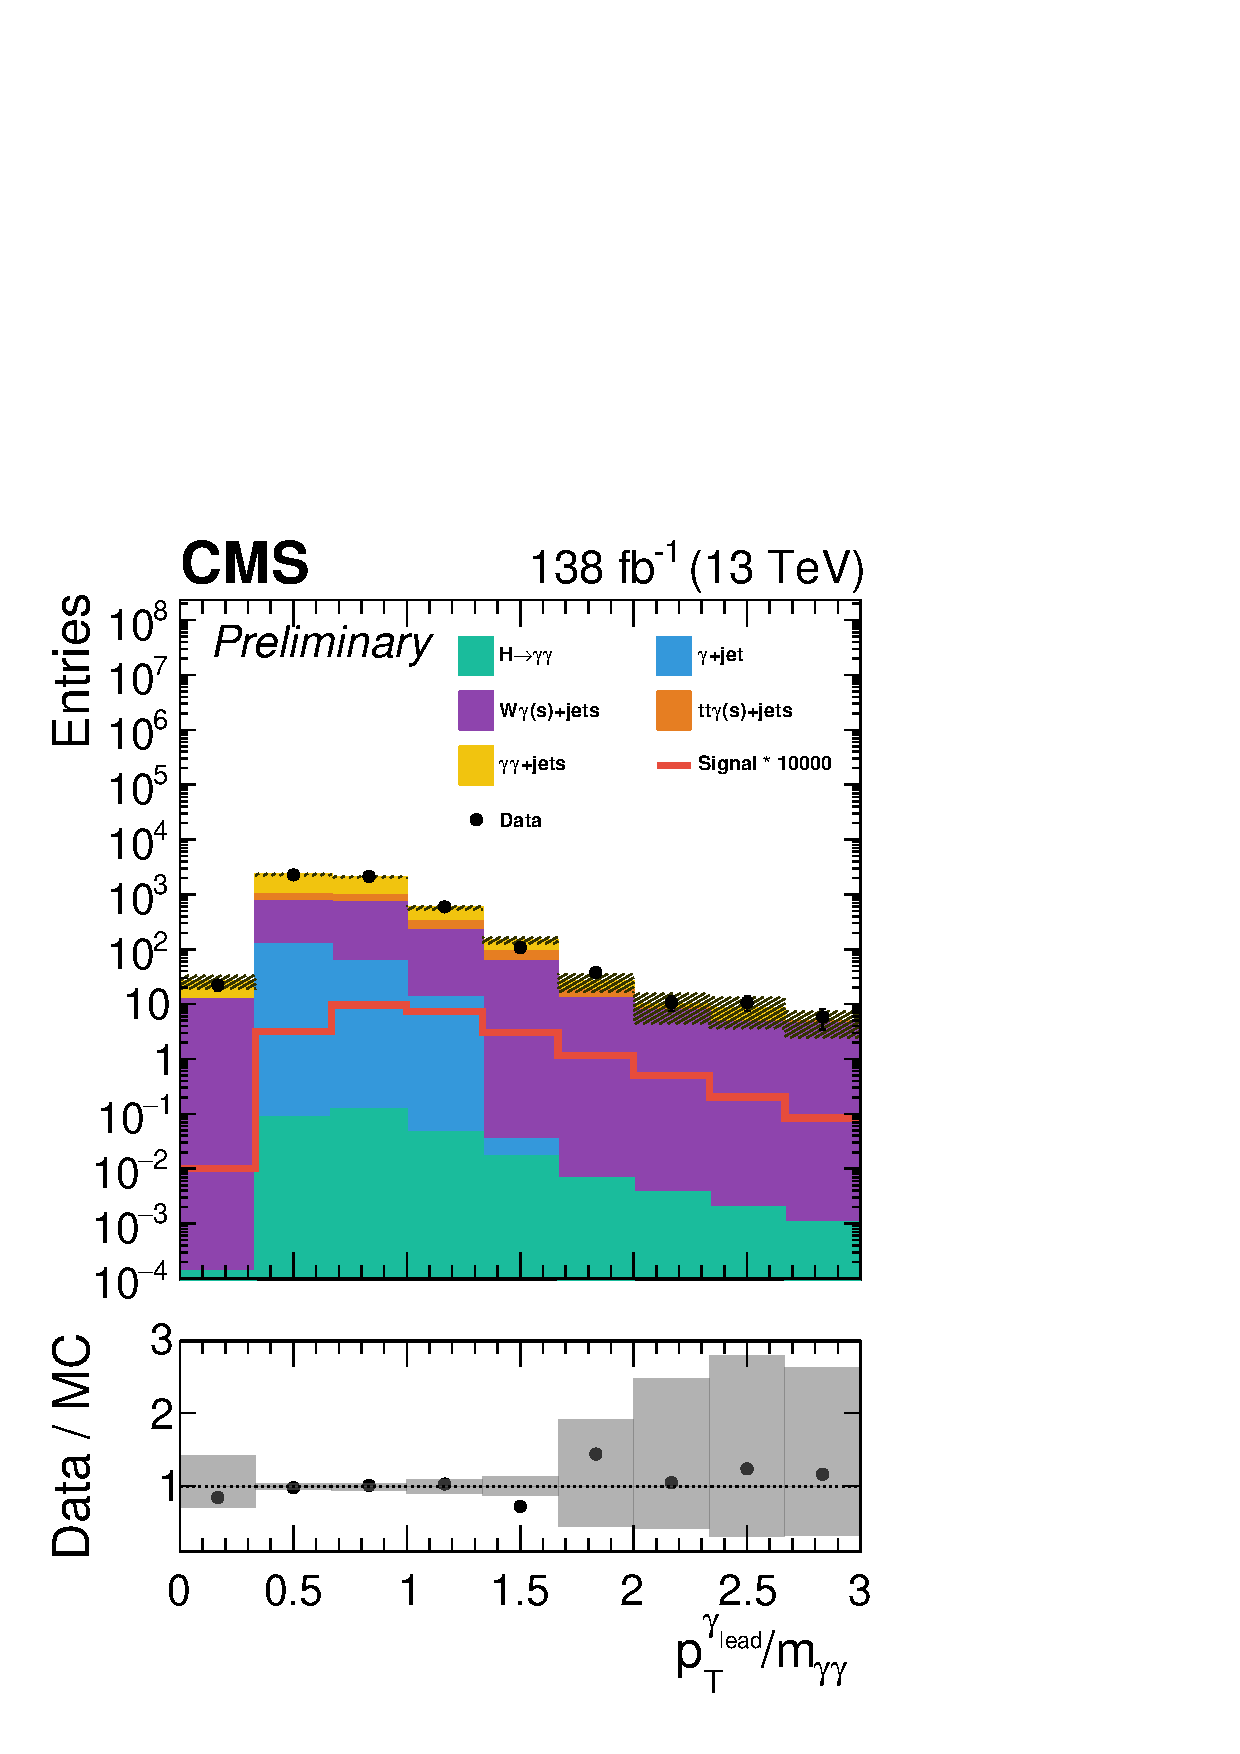
\includegraphics[width=0.47\textwidth]{Sections/HHWWgg/images/DNN/DataMC/DataMC_Scaled_Leading_Photon_pt_FullRegion_log.pdf}}
\subfloat[Scaled Subleading Photon \pt]{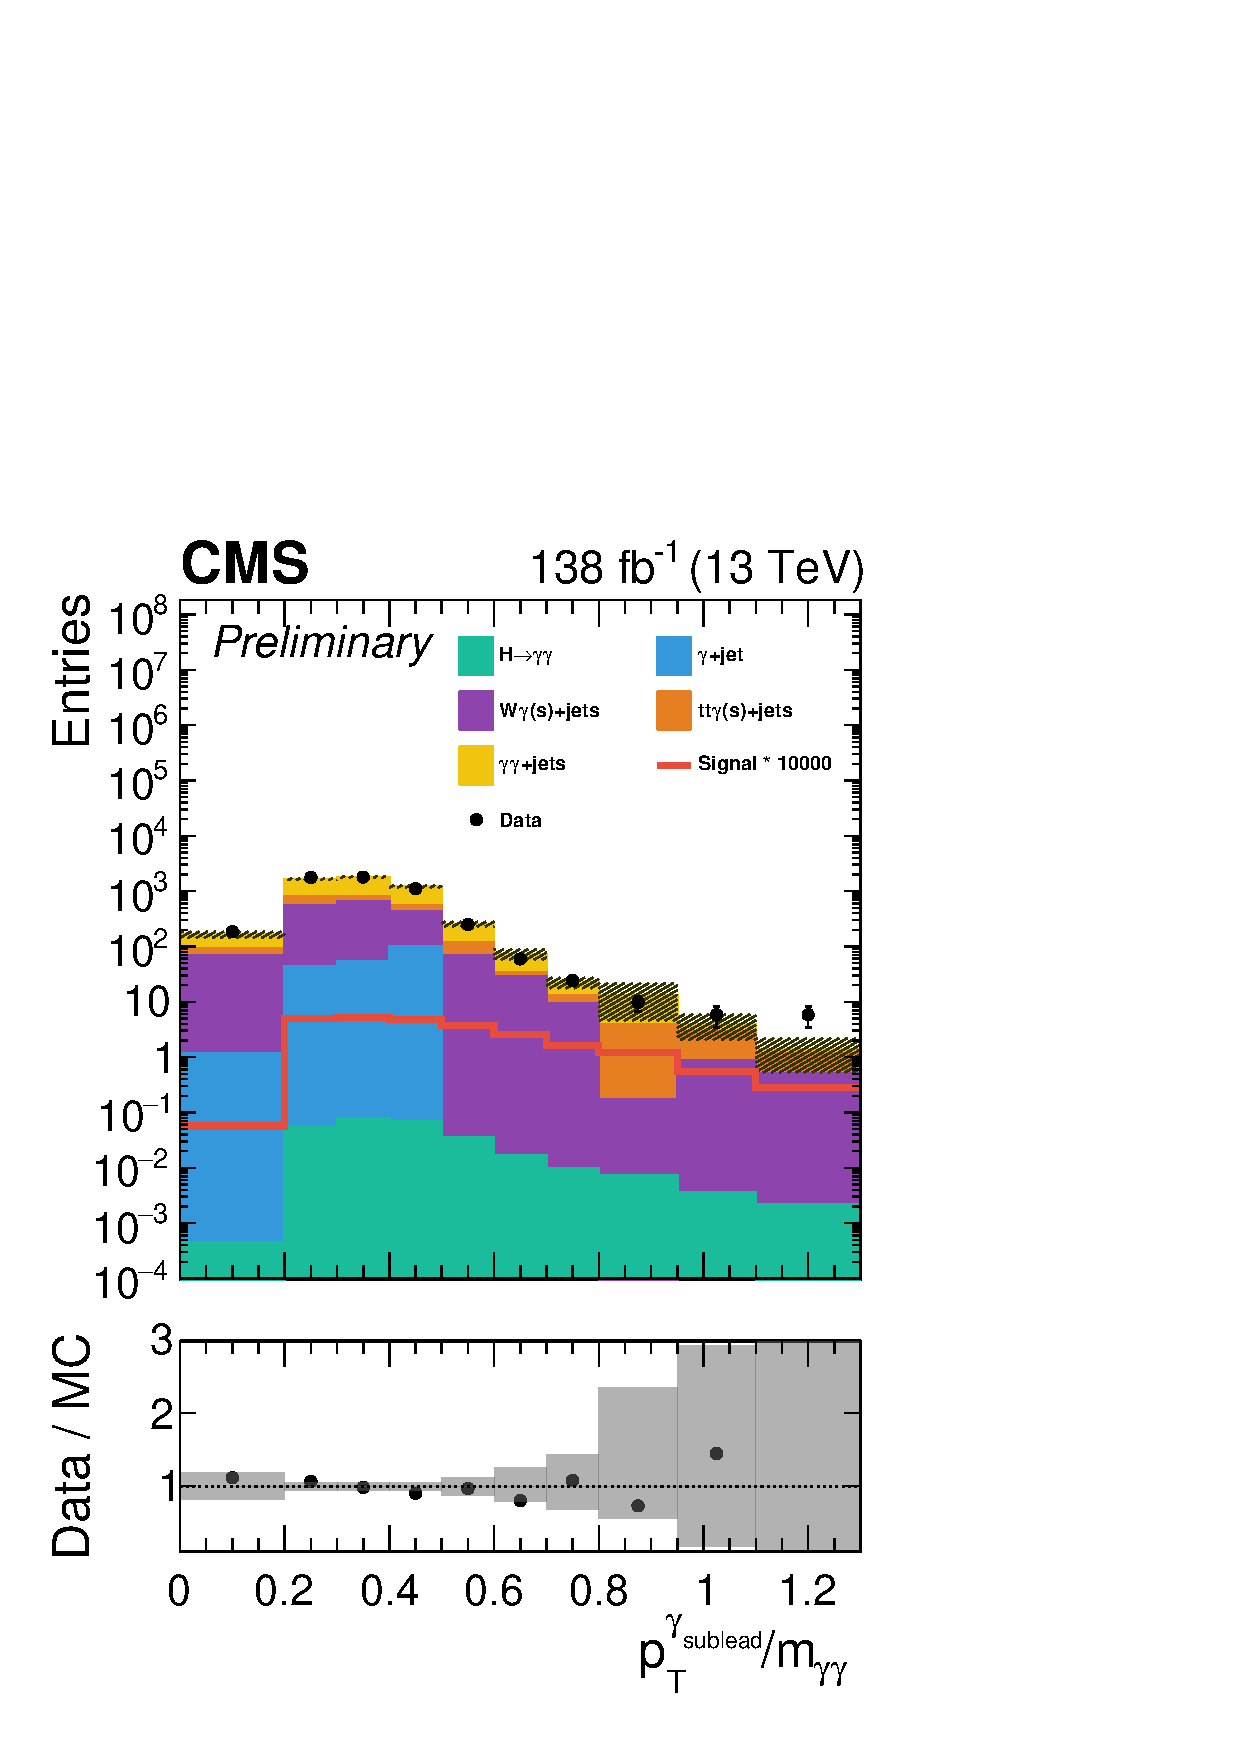
\includegraphics[width=0.47\textwidth]{Sections/HHWWgg/images/DNN/DataMC/DataMC_Scaled_Subleading_Photon_pt_FullRegion_log.pdf}}
\caption{Data/MC ratio of semi-leptonic channel input features in full mass region}
\label{fig:SLDNNFeaturecontrolplots-1}
\end{figure}

\begin{figure}[H]
  \setcounter{subfigure}{0}
  \centering
  \subfloat[Lepton energy]{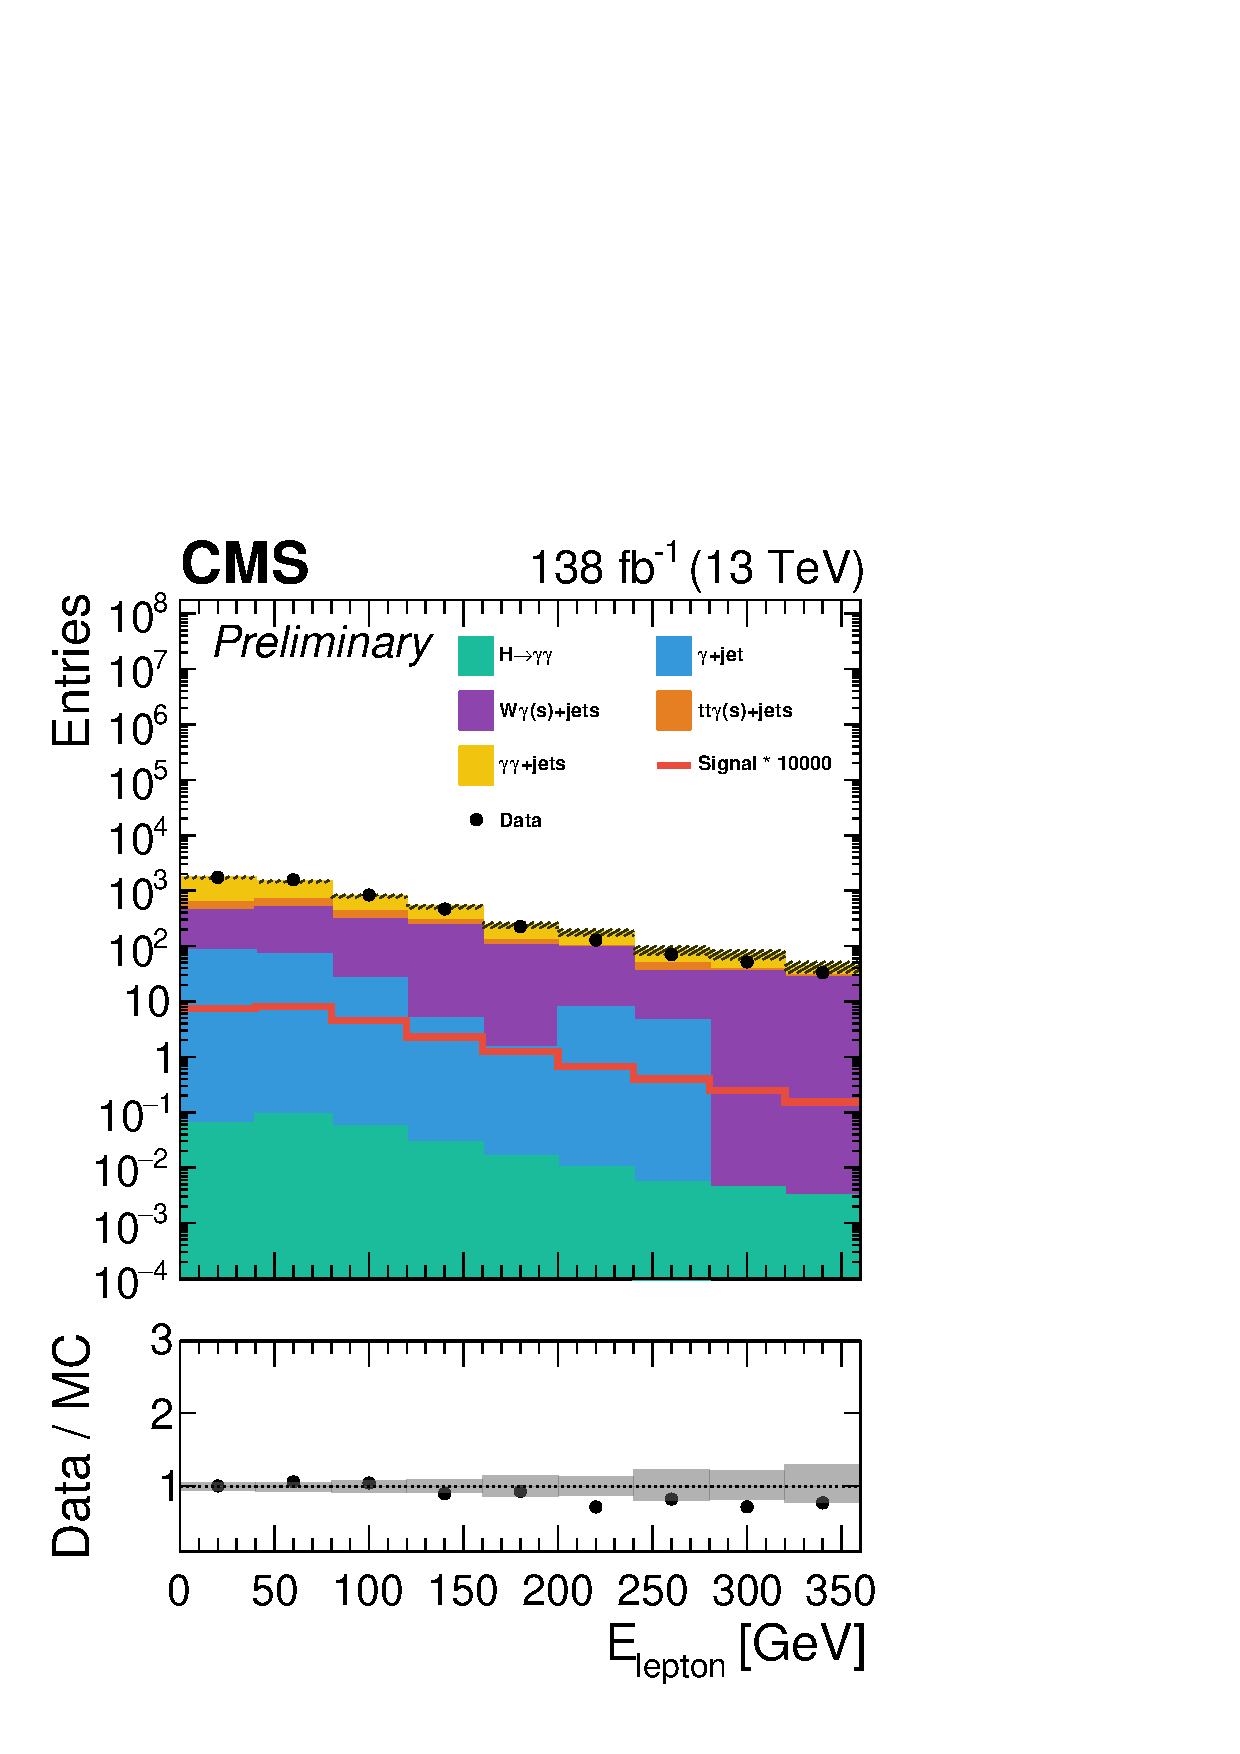
\includegraphics[width=0.47\textwidth]{Sections/HHWWgg/images/DNN/DataMC/DataMC_goodLepton_E_FullRegion_log.pdf}}
  \subfloat[Leading jet \pt \label{fig:lead_jet_pt}]{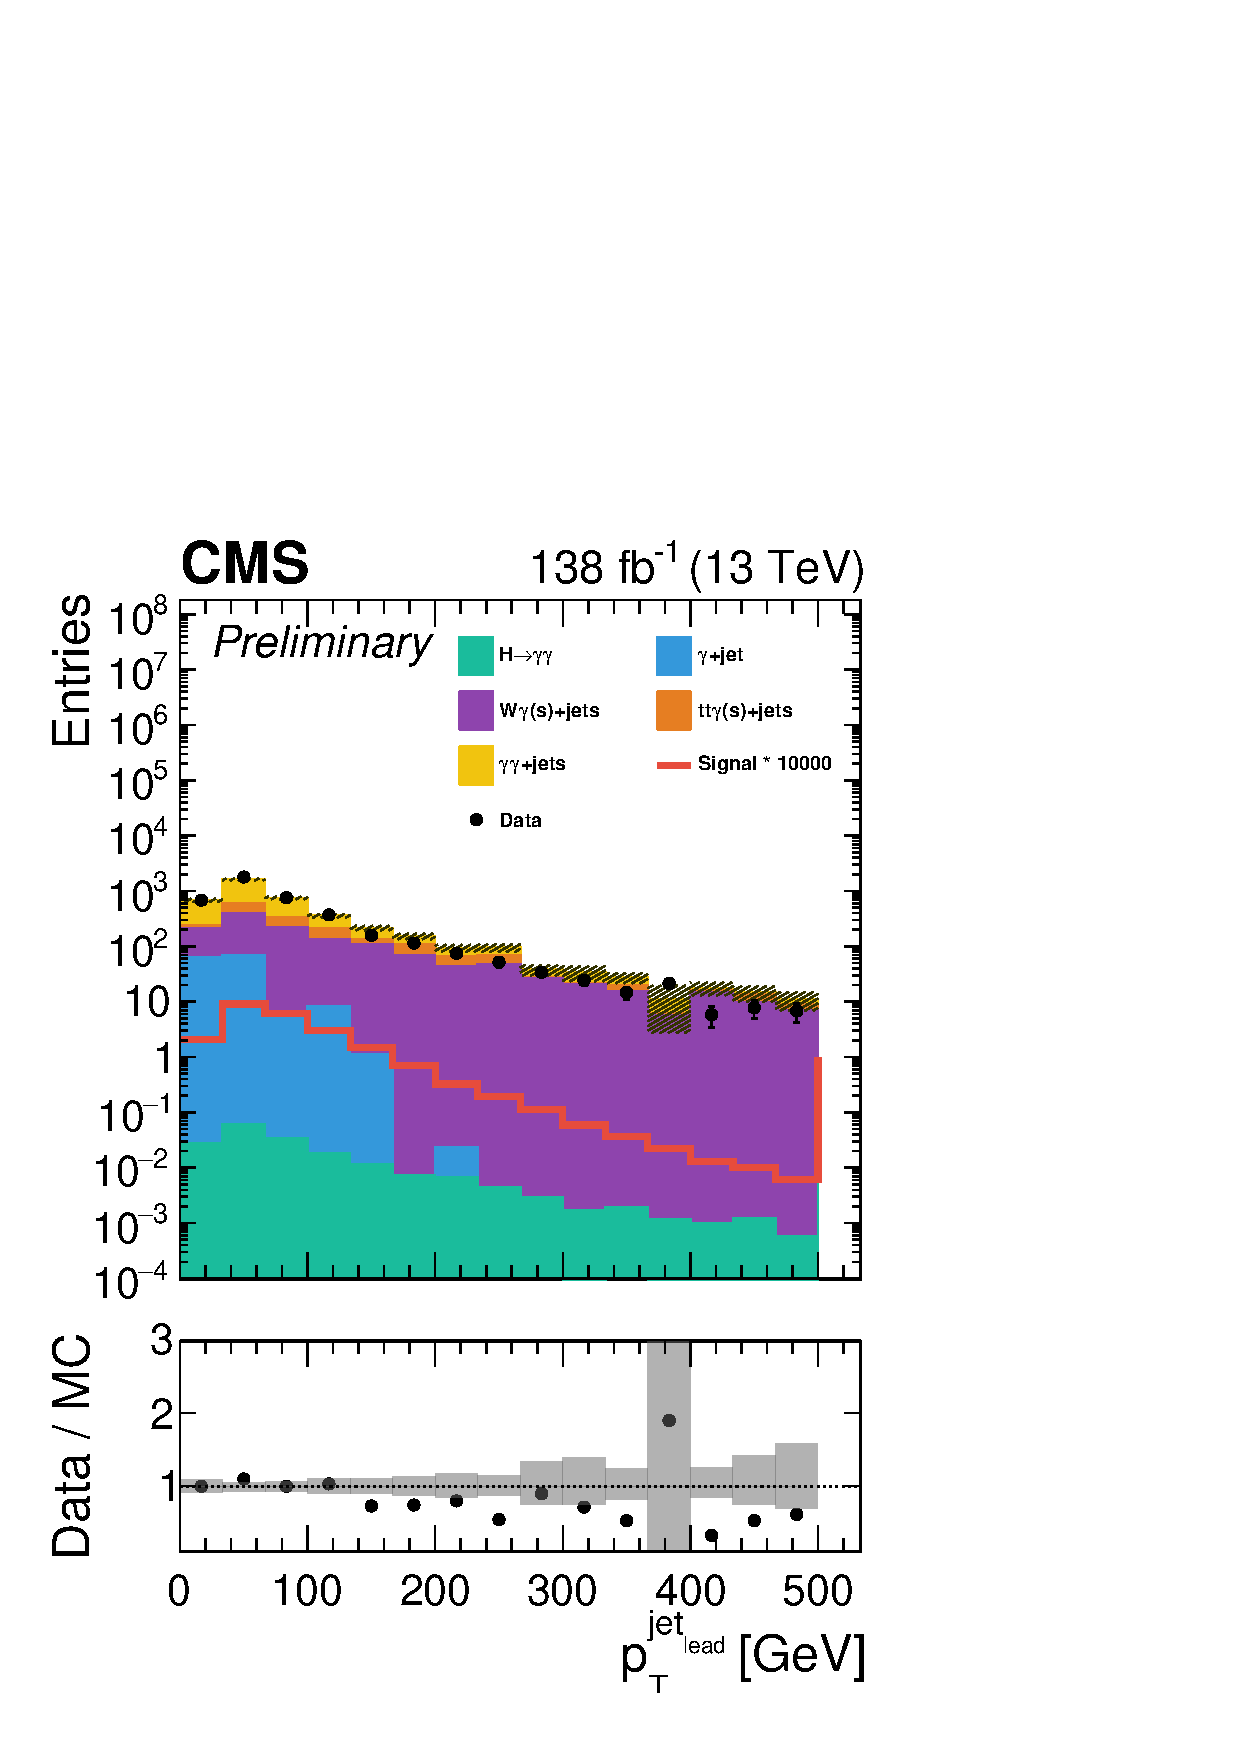
\includegraphics[width=0.47\textwidth]{Sections/HHWWgg/images/DNN/DataMC/DataMC_goodJets_0_pt_FullRegion_log.pdf}}
  \caption{Data/MC ratio of semi-leptonic channel input features in full mass region}
  \label{fig:SLDNNFeaturecontrolplots-2}
\end{figure}

\begin{table}[H]
  \begin{center}
          \begin{tabular}{c|c|c}
                  MC Sample & Unweighted & Weighted \\ \hline
                  DiPhoJetsBox\_MGG-80toInf & 5108 & 581.97343 \\
                  GJet\_40toInf & 110 & 48.26491 \\
                  tt$\gamma\gamma+$0Jets & 4633 & 17.01703 \\
                  tt$\gamma+$Jets & 1564 & 52.52178 \\
                  tt$+$Jets & 288 & 51.77128 \\
                  W1Jets\_pT\_150-250 & 1298 & 64.88303 \\
                  W1Jets\_pT\_250-400 & 341 & 7.42416 \\
                  W1Jets\_pT\_400-inf & 217 & 1.80622 \\
                  W1Jets\_pT\_50-150 & 23 & 13.60197 \\
                  W2Jets\_pT\_150-250 & 1612 & 60.29933 \\
                  W2Jets\_pT\_250-400 & 777 & 12.25016 \\
                  W2Jets\_pT\_400-inf & 531 & 3.05085 \\
                  W2Jets\_pT\_50-150 & 59 & 27.52279 \\
                  WGGJets & 360 & 132.12192 \\
                  WGJJToLNu\_EWK\_QCD & 140 & 30.91906 \\
                  ttWJets & 74 & 0.5721 \\ \hline                
          \end{tabular}
  \captionof{table}{Unweighted and weighted training MC yields in the \mgg sideband region, including semi-leptonic training pre-selections and only events with a DNN output score $>$ 0.1. \label{tab:SL_DNN_Background_yields}}
  \end{center}
\end{table}


\begin{figure}
\caption{Pairwise Spearman's correlation (monotonic relationships) between semileptonic channel DNN input features.}
\setlength{\unitlength}{1mm}
\begin{center}
\mbox{
\includegraphics*[height=150mm]{Sections/HHWWgg/images/DNN/correlation_plot.pdf}
  }
\end{center}
\label{fig:inputvarcorrelation}
\end{figure}

% \begin{figure}[H]
%   \setcounter{subfigure}{0}
%   \centering
%   \subfloat[All Shapley scores]{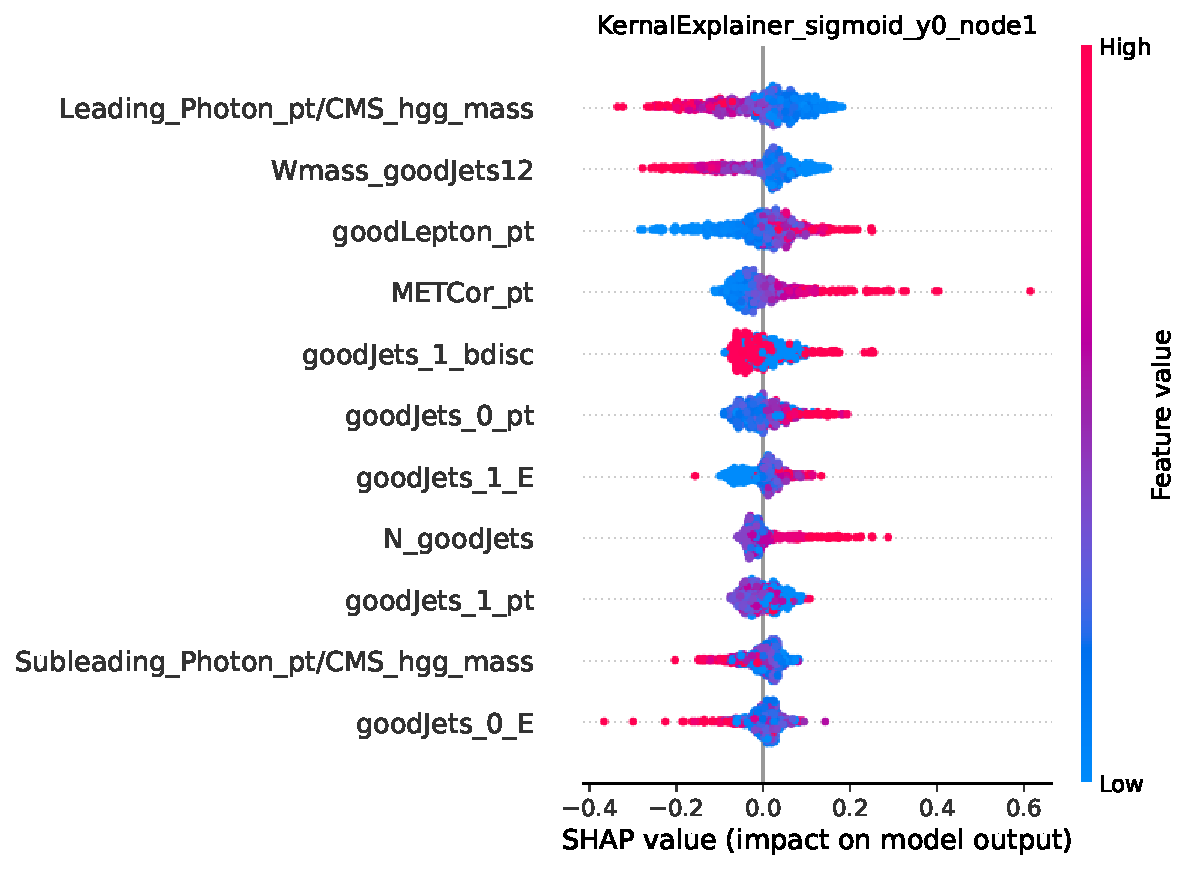
\includegraphics[width=0.45\textwidth]{Sections/HHWWgg/images/DNN/KernalExplainer_sigmoid_y0_node1.pdf}}
%   %\qquad
%   \subfloat[Average Shapley score magnitudes]{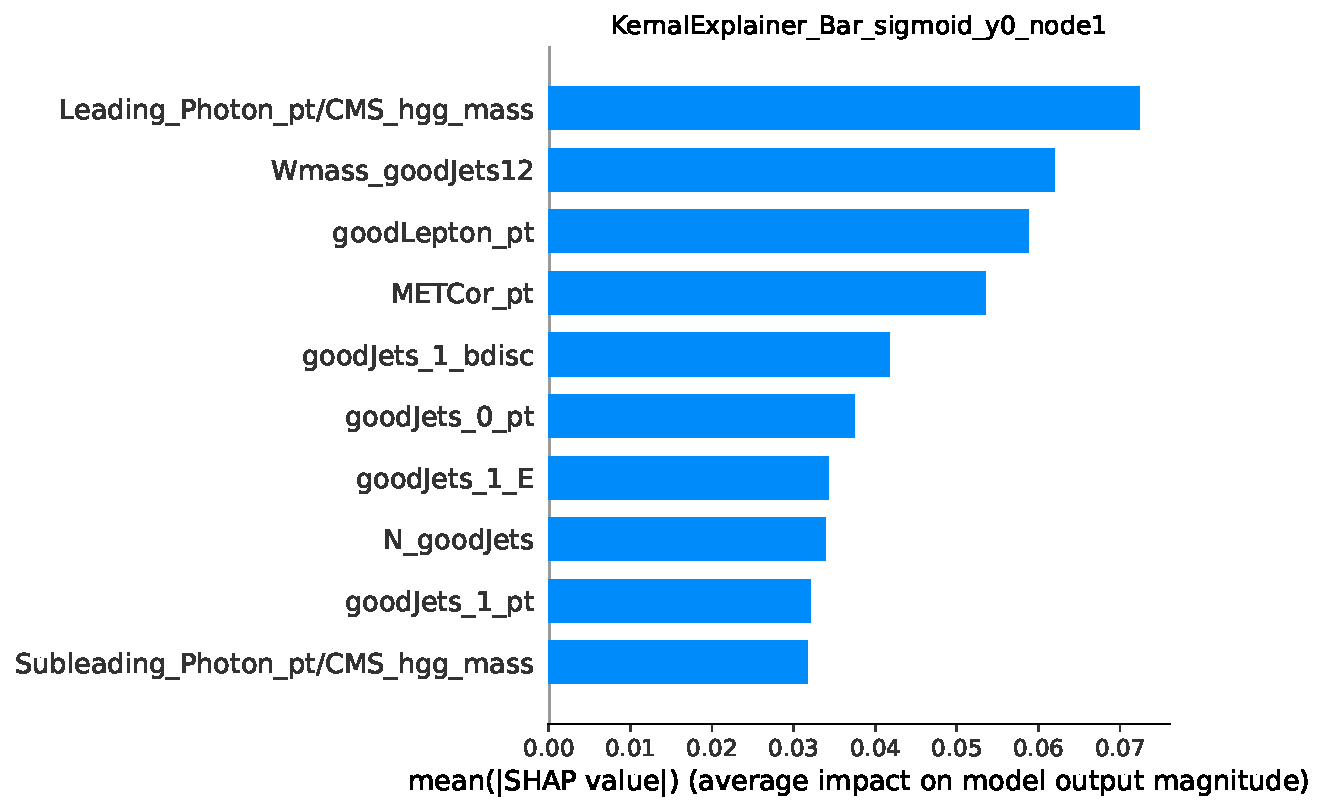
\includegraphics[width=0.45\textwidth]{Sections/HHWWgg/images/DNN/KernalExplainer_Bar_sigmoid_y0_node1.pdf}}
%   \caption{Semi-leptonic channel DNN input feature ranking according to Shapely values in the H class}
%   \label{fig:SLfeatureranking_H}
% \end{figure} 

% \begin{figure}[H]
%   \setcounter{subfigure}{0}
%   \centering
%   \subfloat[All Shapley scores]{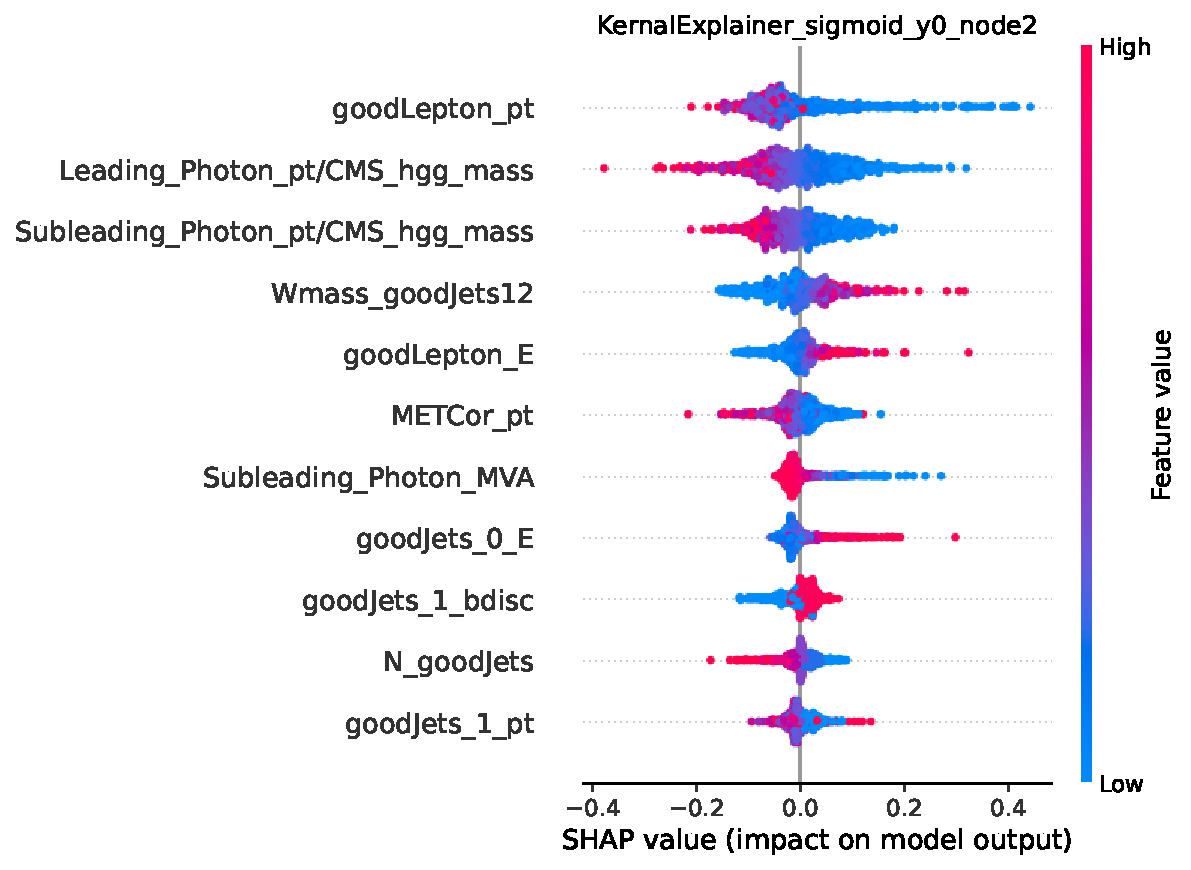
\includegraphics[width=0.45\textwidth]{Sections/HHWWgg/images/DNN/KernalExplainer_sigmoid_y0_node2.pdf}}
%   %\qquad
%   \subfloat[Average Shapley score magnitudes]{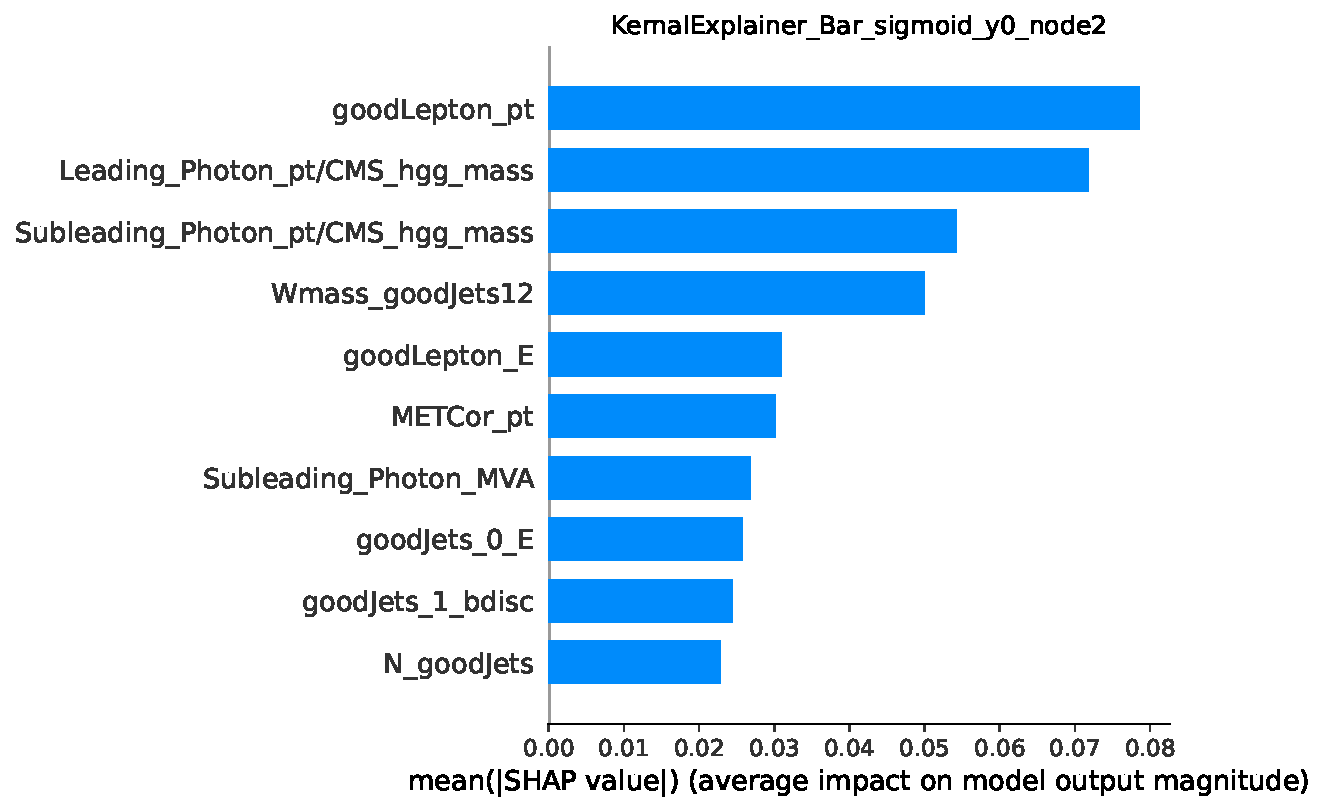
\includegraphics[width=0.45\textwidth]{Sections/HHWWgg/images/DNN/KernalExplainer_Bar_sigmoid_y0_node2.pdf}}
%   \caption{Semi-leptonic channel DNN input feature ranking according to Shapely values in the Continuum background class}
%   \label{fig:SLfeatureranking_bkg}
% \end{figure} 

% The network hyper-parameter settings for the trained semi-leptonic channel DNN can be found in table \ref{tab:hypparams} and the architecture can be found
% in figure \ref{fig:DNNarch}. Several architectures were investigated in an attempt to give the model enough flexibility to model decision boundaries in high-dimensionality 
% phase-space, while ensuring the model is trainable with the size of our dataset. Once the networks architecture was established, a hyper-parameter scan was performed on the number of epochs, learning rate and batch size. 
% The optimal network performance was achieved with the chosen parameters. The performance of networks of a given architecture was found to be relatively robust to further
% fine-tuning of hyper-parameters.

% The output ROC curves from training for each class can be seen in Figures \ref{fig:ROC_HH}, \ref{fig:ROC_H} and \ref{fig:ROC_bkg}, shown together for all 
% training and test sets in Figure \ref{fig:All_ROCs}. The corresponding
% loss vs. epoch trend is shown in Figure \ref{fig:LossVsEpoch} for a test and training set of data, where 90\% of sample events are reserved for training and the other 10\% for the test dataset 
% in order to check for overtraining. Additionally, the normalized HH, H, and Continuum background DNN output scores are plotted for training and test samples to check for overtraining, as shown in Figures \ref{fig:SL_DNN_overfitting_check}, 
% \ref{fig:SL_DNN_overfitting_check_SingleH} and \ref{fig:SL_DNN_overfitting_check_ContBkg}. For 
% all three types of events, HH, H and continuum background, the distributions of the HH, H and continuum background node DNN scores for training and test samples are in agreement, a further indication that there is no overtraining and therefore 
% no loss in sensitivity due to overtraining.

The output DNN score comparison between the data
and MC is shown in Figure \ref{fig:SL_DNN_Score}. In this comparison, events with a DNN score less than 0.1 are removed as they are not used in categorization or signal modeling.

Finally, the output DNN score for data events in the sidebands and signal events in the signal region are shown in Figure \ref{fig:YearByYear_DNN_Scores}, not including 
events with a DNN score less than 0.1 as they are not used in the analysis. Each signal histogram is normalized to an integral of 1, and each data histogram is normalized to the luminosity of the 2018 dataset.
It can be seen that the shapes are very similar per year, and that there is no clear systematic difference when applying the 2017-only trained DNN on 
2016 and 2018 data and signal events. The data histograms are shown in log scale in order to highlight that there are similar DNN score shapes per year which appear similar within statistical uncertainty,
in particular in the high DNN score region which is the most signal sensitive region. 

% \begin{figure}[H]
%   \caption{Semi-Leptonic DNN ROC curve for training and test data: H Class}
%   \setlength{\unitlength}{1mm}
%   \begin{center}
%     \mbox{\includegraphics*[height=100mm]{Sections/HHWWgg/images/DNN/MultiClass_ROC_class_H.pdf}
%     }
%   \end{center}
%   \label{fig:ROC_H}
% \end{figure}

% \begin{figure}[H]
%   \caption{Semi-Leptonic DNN ROC curve for training and test data: Continuum Background class}
%   \setlength{\unitlength}{1mm}
%   \begin{center}
%     \mbox{\includegraphics*[height=100mm]{Sections/HHWWgg/images/DNN/MultiClass_ROC_class_Bkg.pdf}
%     }
%   \end{center}
%   \label{fig:ROC_bkg}
% \end{figure}

% \begin{figure}[H]
%   \setcounter{subfigure}{0}
%   \centering
%   \subfloat[Test samples]{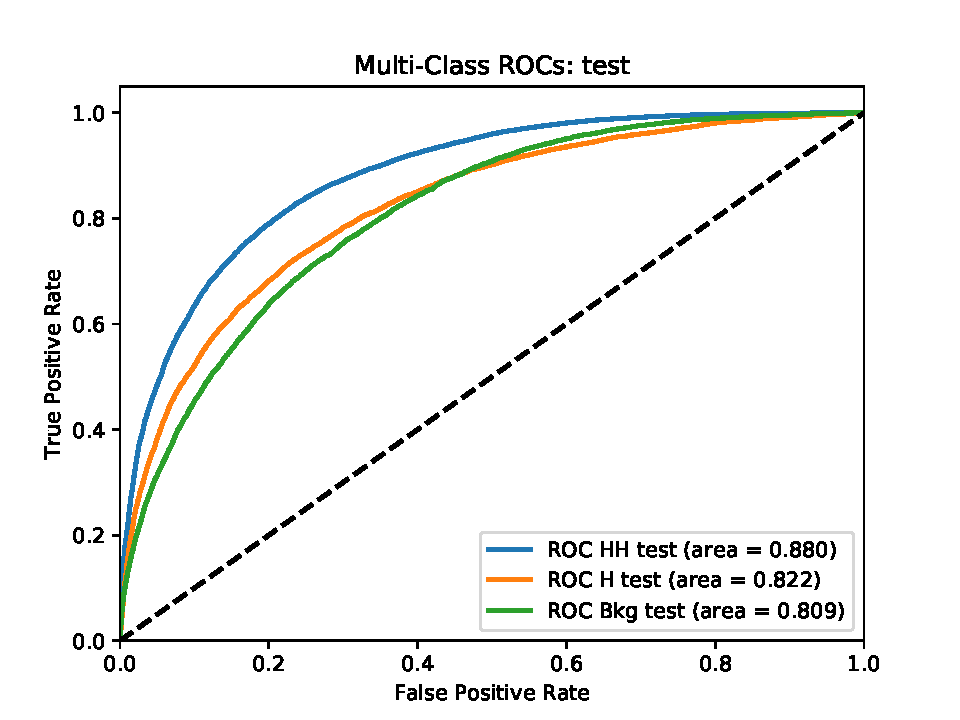
\includegraphics[width=0.45\textwidth]{Sections/HHWWgg/images/DNN/MultiClass_ROC_dataset_test.pdf}}
%   \qquad
%   \subfloat[Training samples]{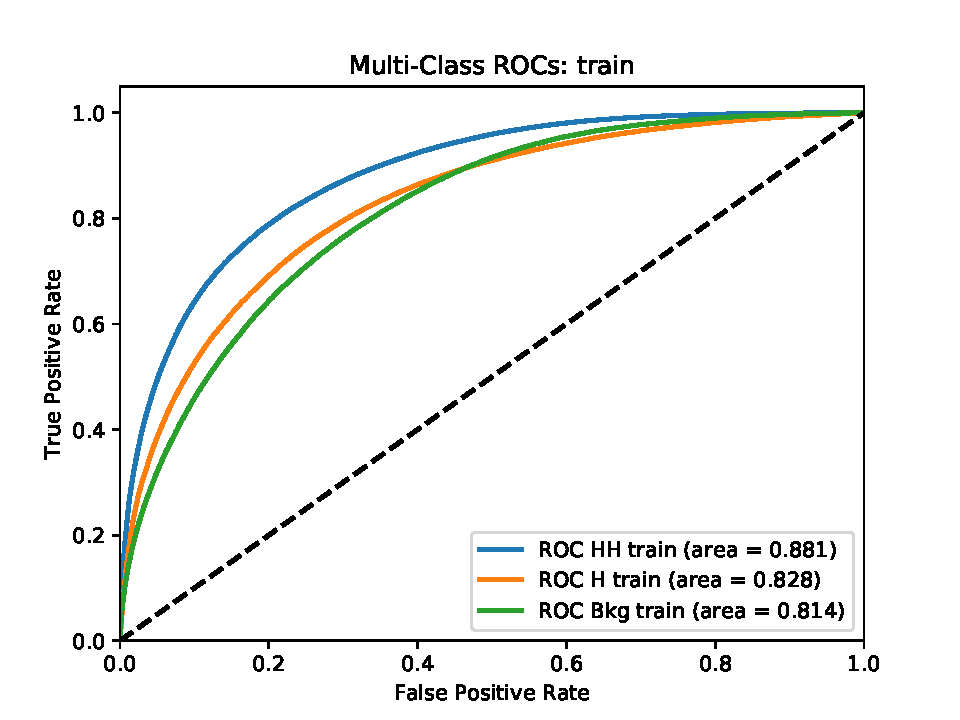
\includegraphics[width=0.45\textwidth]{Sections/HHWWgg/images/DNN/MultiClass_ROC_dataset_train.pdf}}
%   \caption{ROC curves of three MultiClass nodes}
%   \label{fig:All_ROCs}
% \end{figure} 

% \begin{figure}[H]
%   \caption{Semi-Leptonic DNN loss vs. epoch for training and test data}
%   \setlength{\unitlength}{1mm}
%   \begin{center}
%     \mbox{\includegraphics*[height=100mm]{Sections/HHWWgg/images/DNN/history_loss.pdf}
    
%     }
%   \end{center}
%   \label{fig:LossVsEpoch}
% \end{figure}

% \begin{figure}[H]
%   \setlength{\unitlength}{1mm}
%   \begin{center}
%     \mbox{\includegraphics*[height=100mm]{Sections/HHWWgg/images/DNN/overfitting_plot_Single_H_Non-Categorised.pdf}
%     }
%   \end{center}
%   \caption{Normalized Single Higgs DNN score distributions for the three semileptonic DNN nodes, shown for training and test events.}
%   \label{fig:SL_DNN_overfitting_check_SingleH}
% \end{figure}

% \begin{figure}[H]
%   \setlength{\unitlength}{1mm}
%   \begin{center}
%     \mbox{\includegraphics*[height=100mm]{Sections/HHWWgg/images/DNN/overfitting_plot_Cont_Bkg_Non-Categorised.pdf}
%     }
%   \end{center}
%   \caption{Normalized Continuum Background DNN score distributions for the three semileptonic DNN nodes, shown for training and test events.}
%   \label{fig:SL_DNN_overfitting_check_ContBkg}
% \end{figure}


% \begin{table}[H]
%     \begin{center}
%   \caption{Hyper-parameter settings for semi-leptonic channel DNN}
%   \resizebox{100mm}{!}{
%   \begin{tabular}{| l | l |}
%     \hline
%     Hyper-parameter & Setting \\
%     \hline
%     Epochs & 500 \\
%     Batch size &  500 \\
%     Learning rate & 0.0001 \\
%     Optimiser & Nadam \\
%     Loss function & categorical$\_$crossentropy \\
%     Kernel initialiser & glorot normal \\
%     Hidden layer activation functions & ReLU \\
%     Output layer activation function & softmax \\
%     \hline
%   \end{tabular}
%   }
%   \label{tab:hypparams}
%   \end{center}
% \end{table}

% \begin{figure}
%     \caption{Schematic of semi-leptonic DNN model architecture. The sequential DNN model shows the various layer names along with the dimensions of the input and output vectors. One can see that a vector of 29 input variables is condensed down into a binary output value in the last layer.}
%   \setlength{\unitlength}{1mm}
%   \begin{center}
%     \mbox{\includegraphics*[height=150mm]{Sections/HHWWgg/images/DNN/model_schematic.pdf}
%     }
%   \end{center}
%   \label{fig:DNNarch}
% \end{figure}

% \begin{figure}[H]
%   \setcounter{subfigure}{0}
%   \centering
%   \subfloat[Linear y scale]{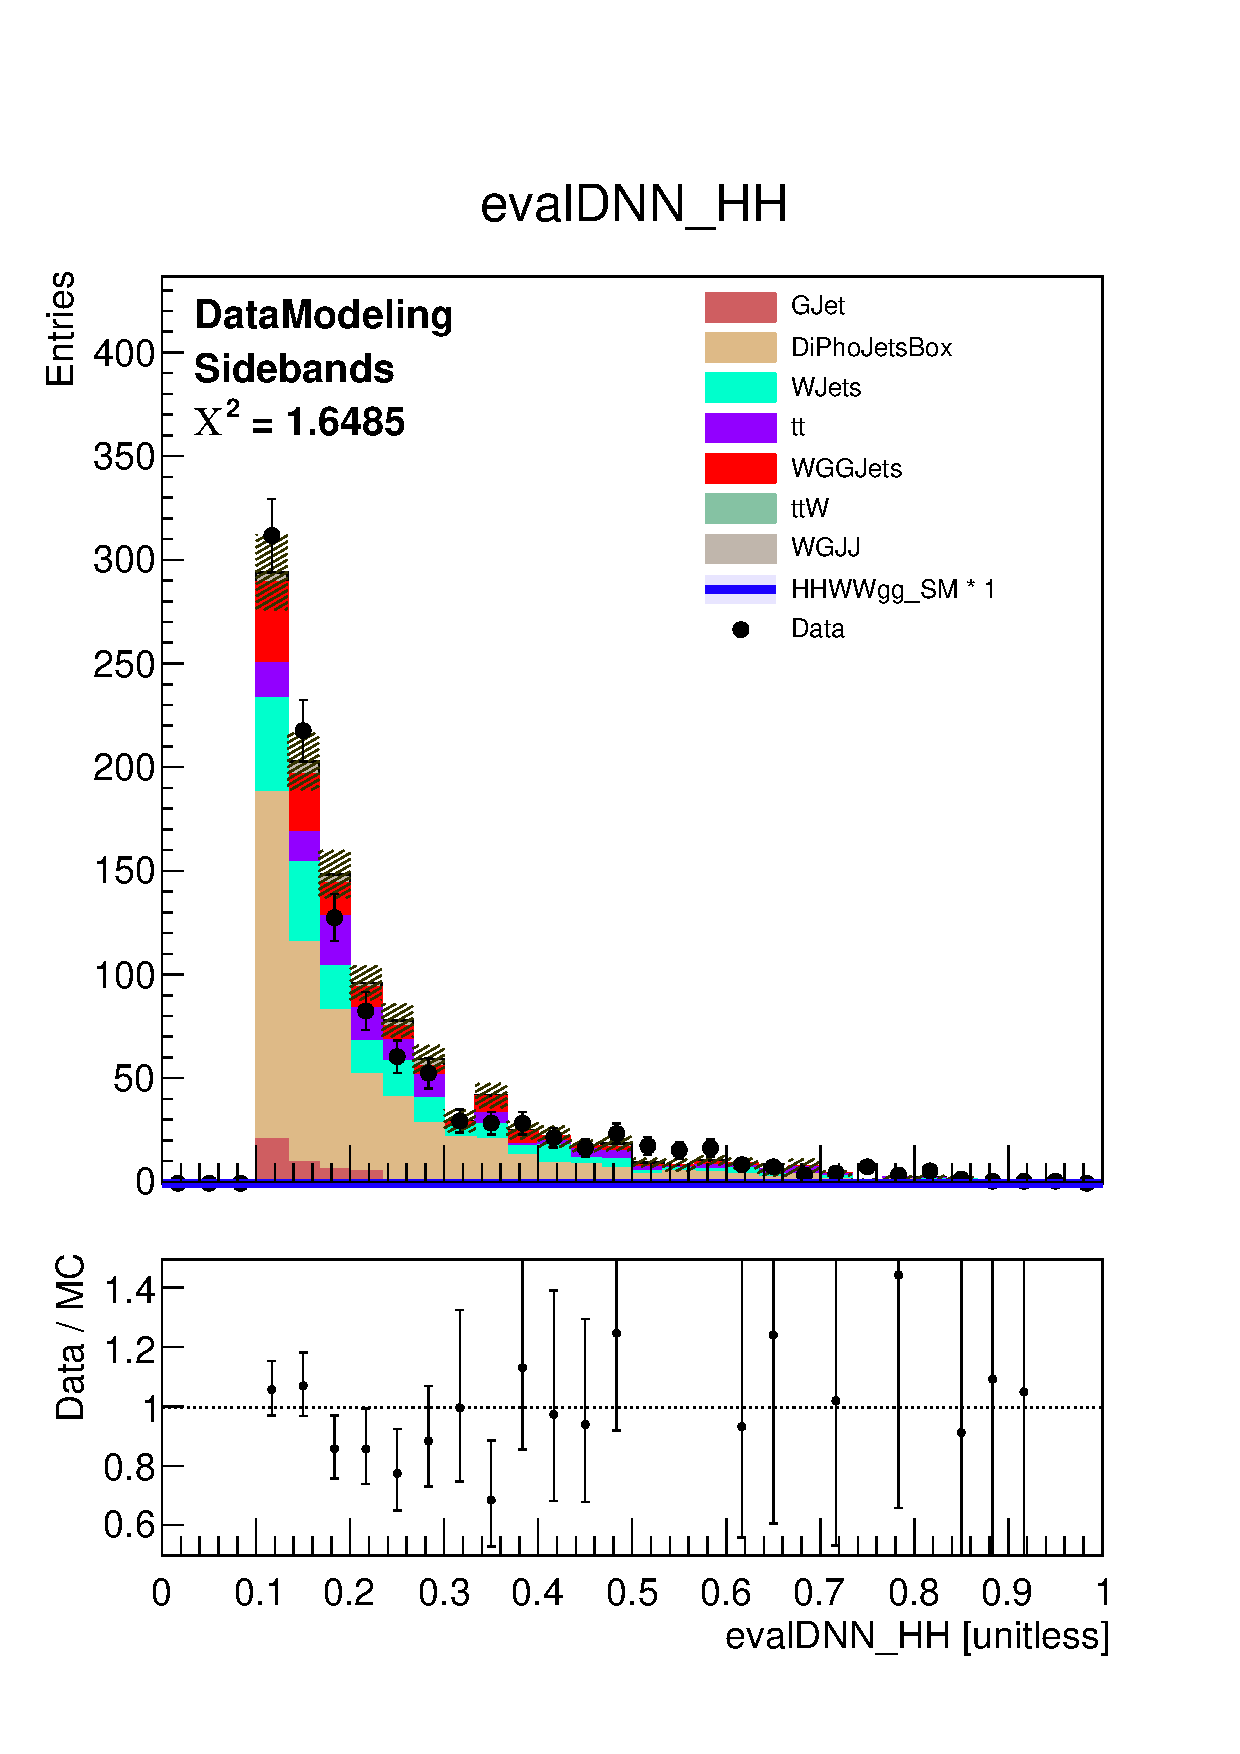
\includegraphics[width=0.45\textwidth]{Sections/HHWWgg/images/DNN/DataMC/DataMC_evalDNN_HH_SB_nonLog.pdf}}
%   \qquad
%   \subfloat[Logarithmic y scale]{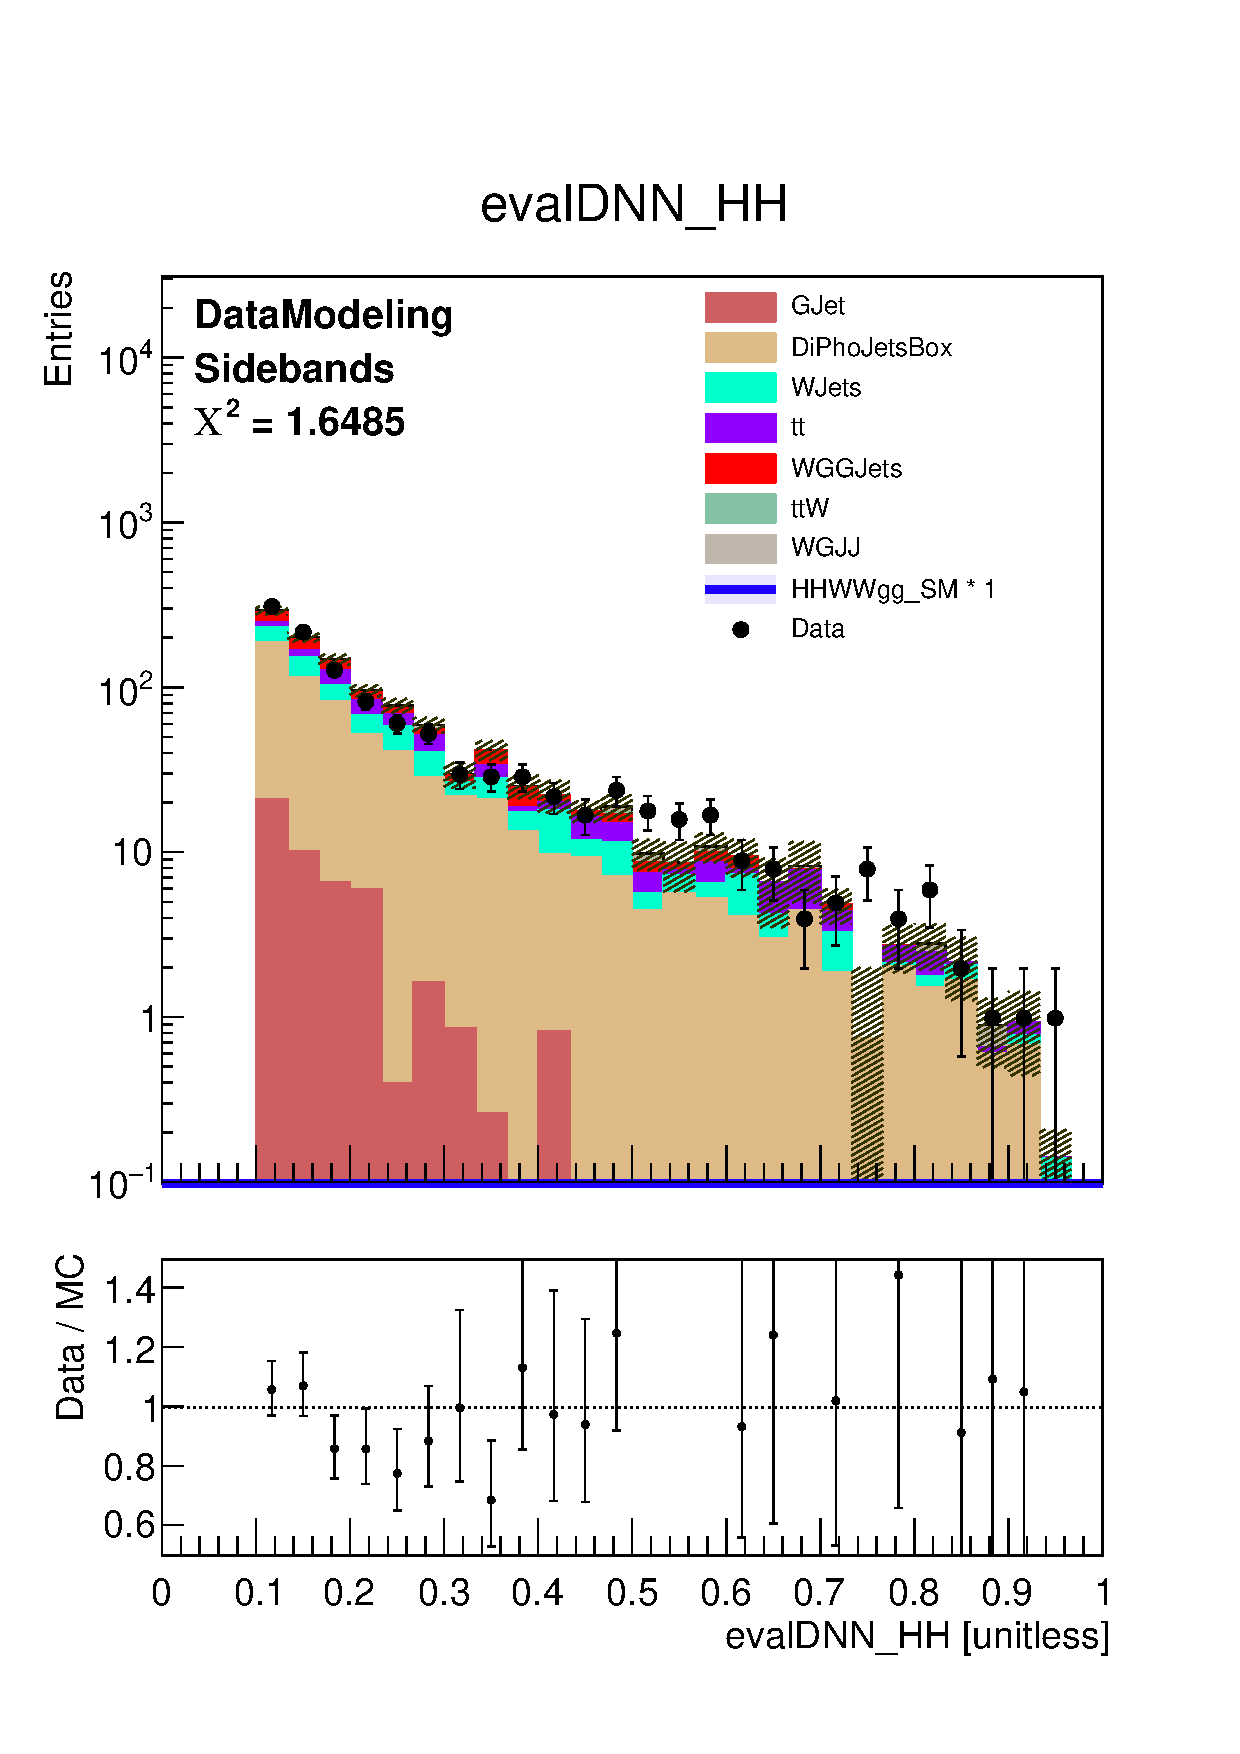
\includegraphics[width=0.45\textwidth]{Sections/HHWWgg/images/DNN/DataMC/DataMC_evalDNN_HH_SB_log.pdf}}
%   \caption{Output DNN score for 2017 data and MC in the signal sideband. A logarithmic y scale version is included in order to see the low statistics bins.}
%   \label{fig:DNNscore_Data_MC}
% \end{figure} 

\begin{figure}[H]
    \centering
    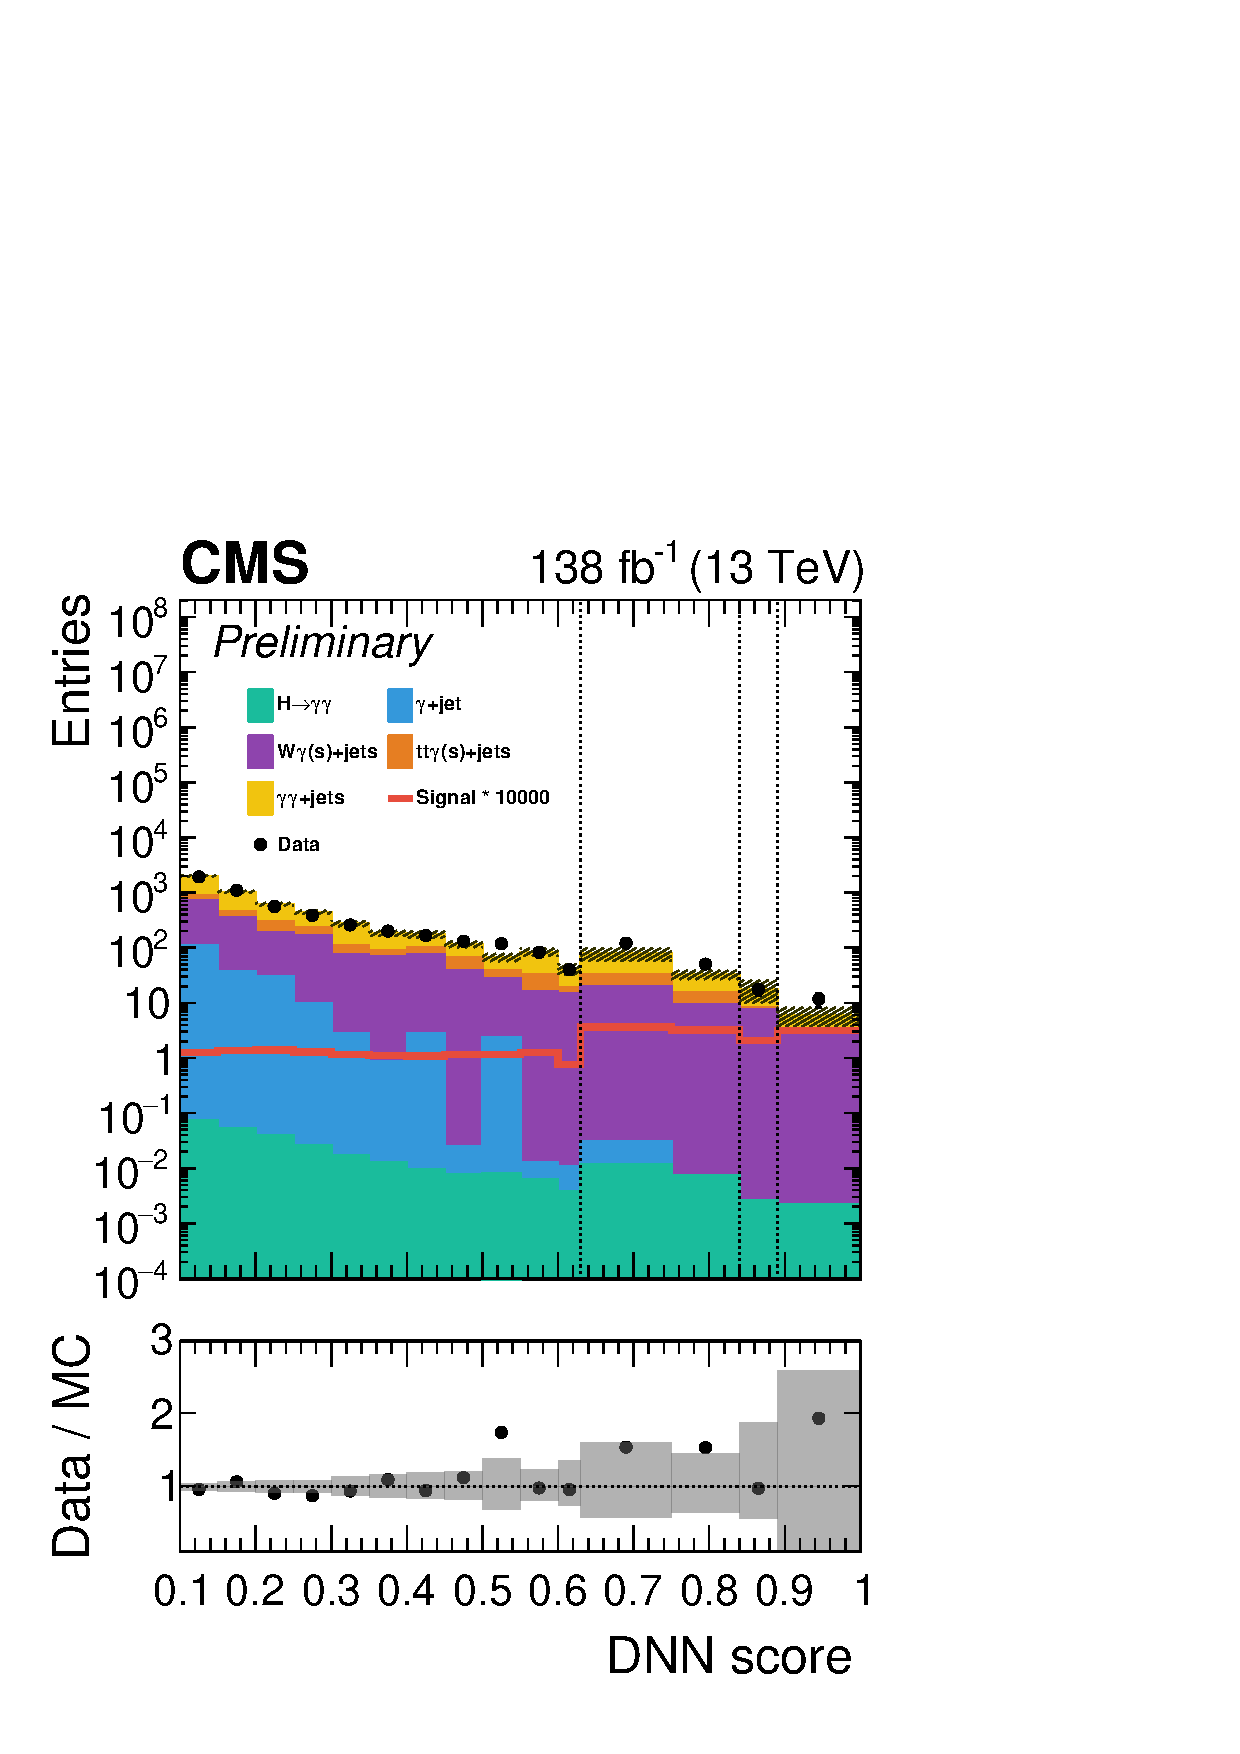
\includegraphics[width=\textwidth]{Sections/HHWWgg/images/DNN/DataMC/DataMC_evalDNN_HH_FullRegion_log.pdf}
    \caption{DNN output score between data and MC, using Run 2 dataset and 2017 MC scaled to Run 2 lumi.}
    \label{fig:SL_DNN_Score}
\end{figure}

\begin{figure}[H]
  \setcounter{subfigure}{0}
  \centering
  \subfloat[Data in data sideband, each year scaled to 2018 luminosity]{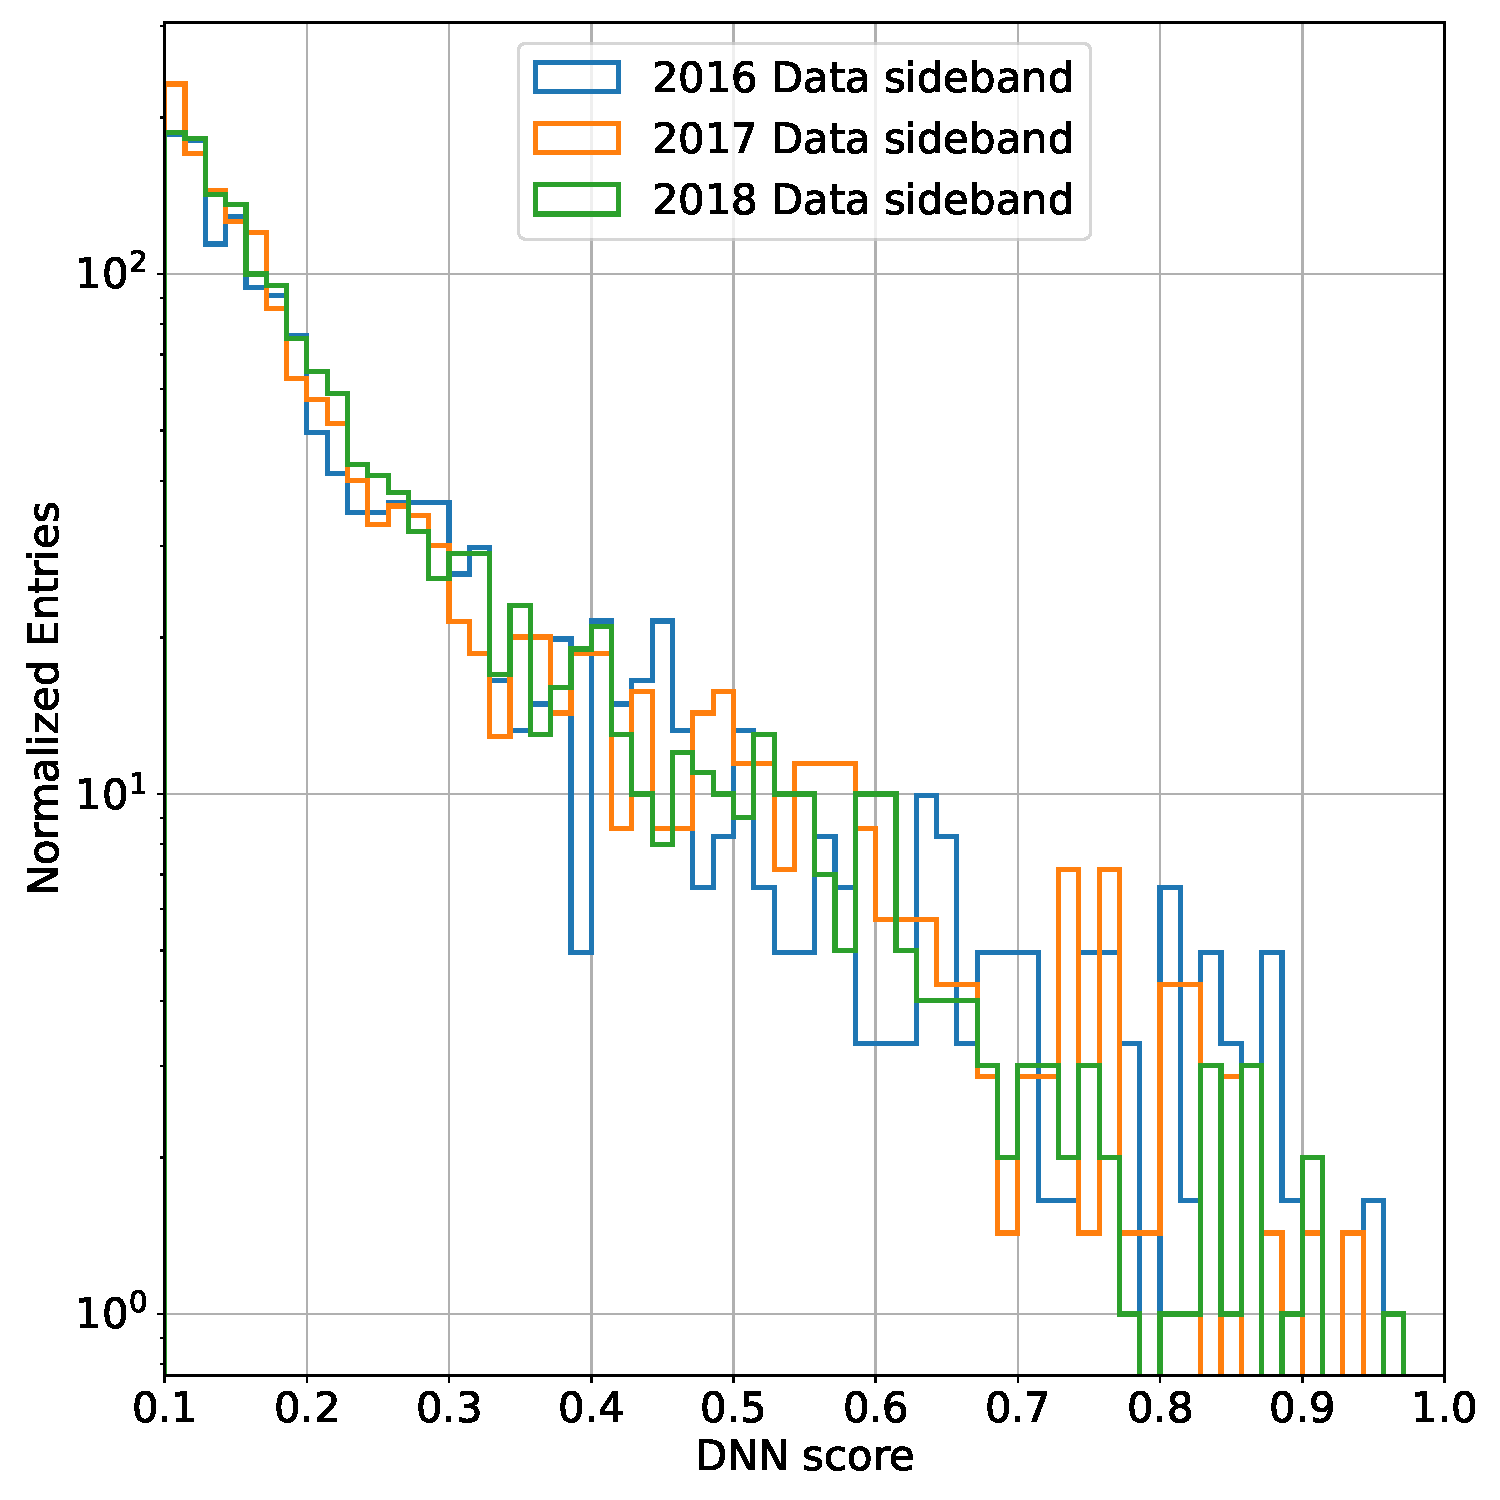
\includegraphics[width=0.45\textwidth]{Sections/HHWWgg/images/DNN/YearByYear_SLDNN_scores_Data_log.pdf}}
  \qquad
  \subfloat[Signal in signal region, each histogram normalized to an integral of 1]{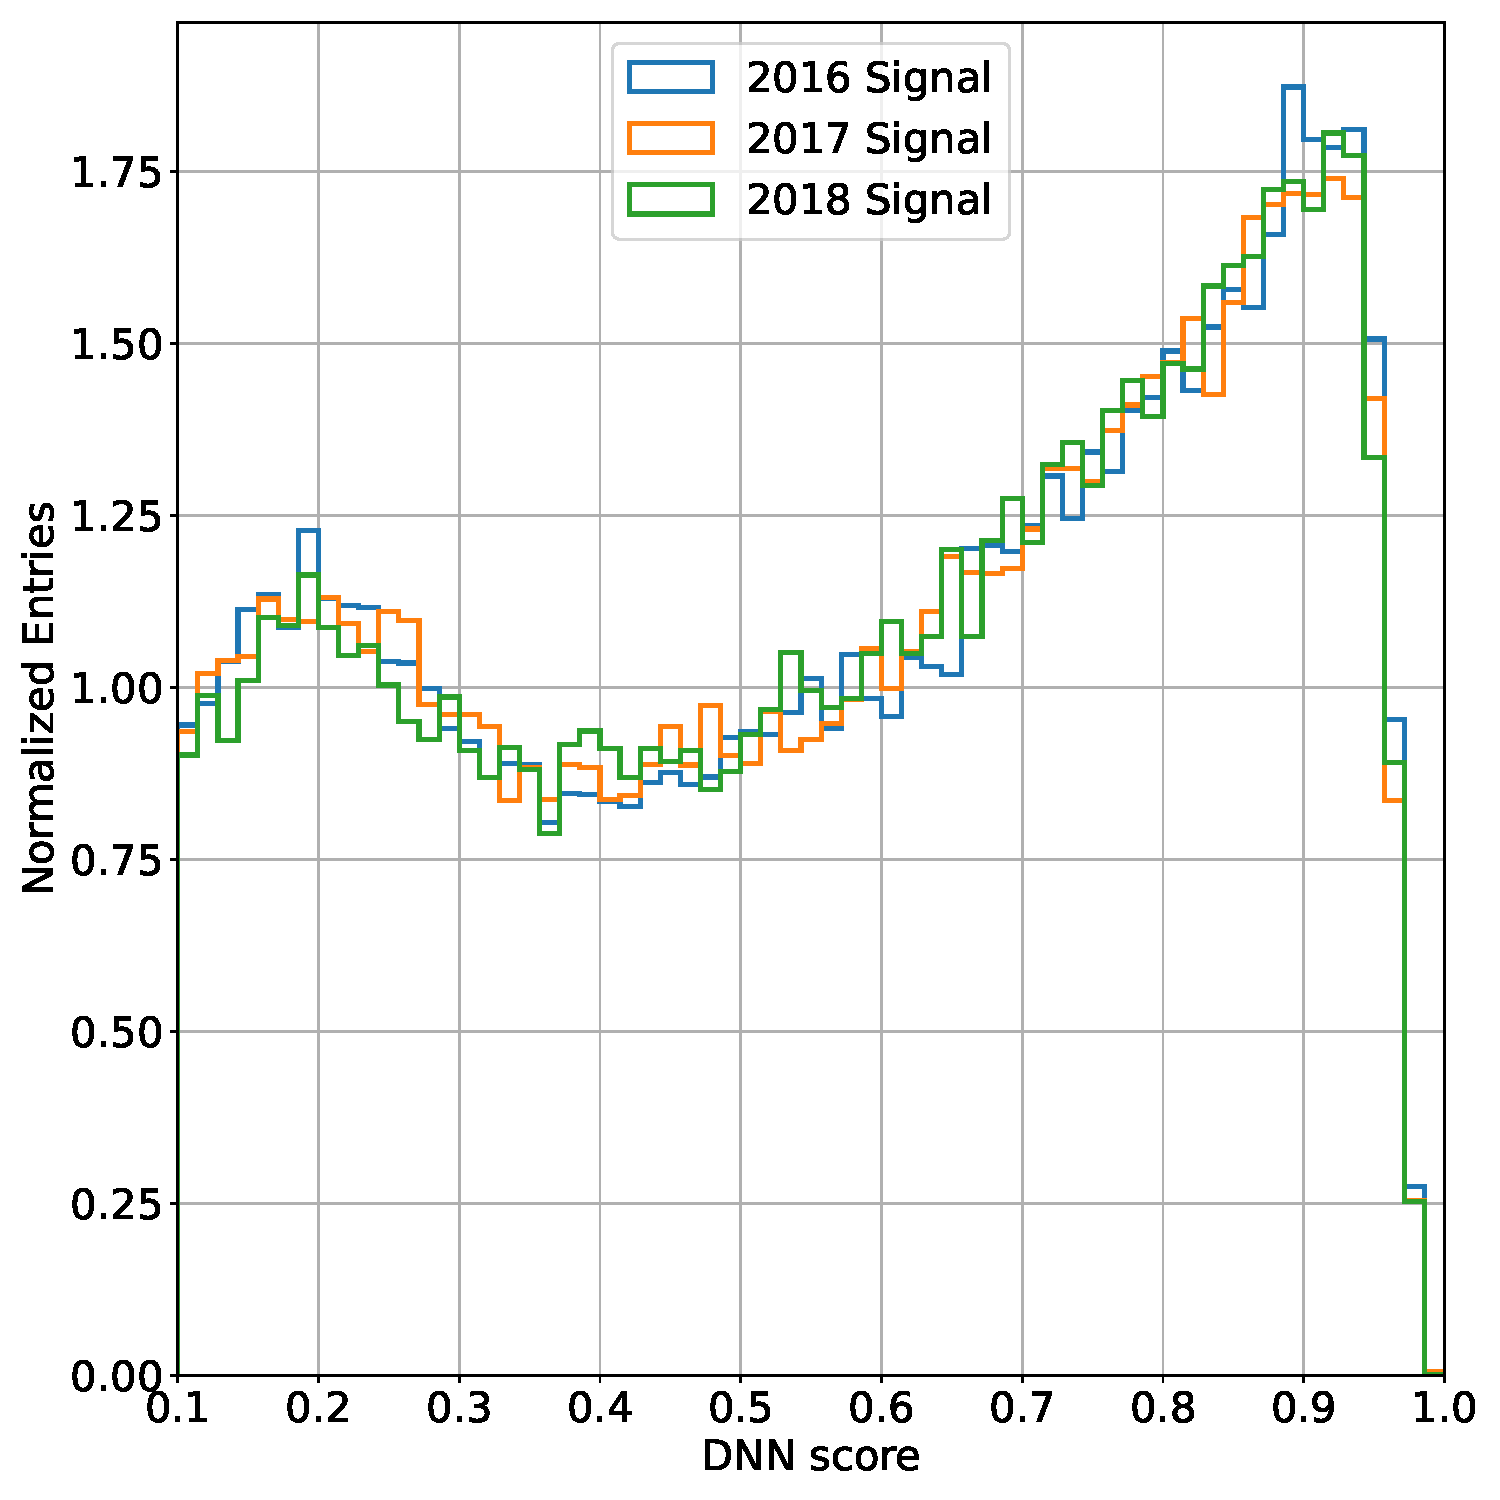
\includegraphics[width=0.45\textwidth]{Sections/HHWWgg/images/DNN/YearByYear_SLDNN_scores_sig.pdf}}
  \caption{DNN output score of data events in the sideband region (a), and HH simulation events in the signal region (b), for each separate year.}
  \label{fig:YearByYear_DNN_Scores}
\end{figure} 

% \begin{figure}[H]
%   \setcounter{subfigure}{0}
%   \centering
%   \subfloat[Without sideband scale]{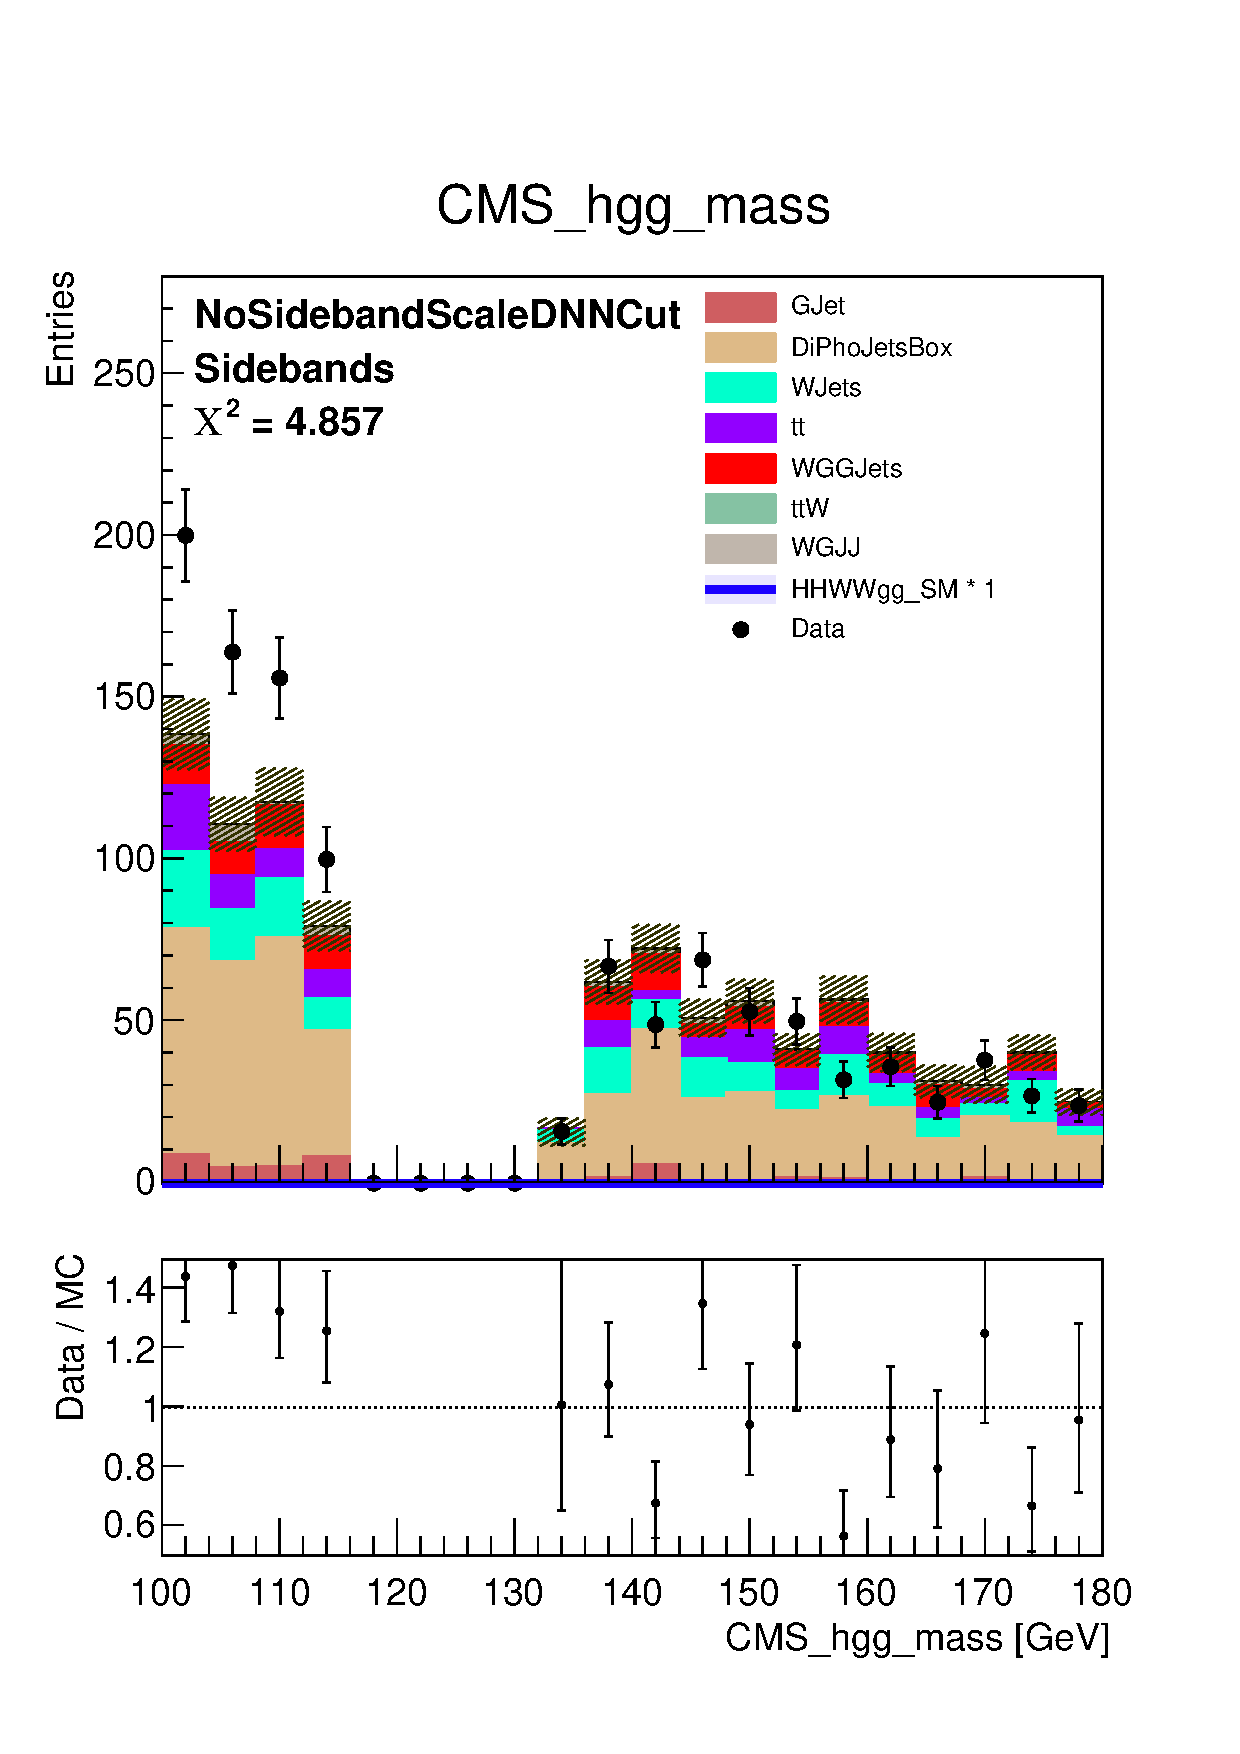
\includegraphics[width=0.45\textwidth]{Sections/HHWWgg/images/DNN/DataMC_CMS_hgg_mass_SB_NoSidebandScaleFactor_nonLog.pdf}}
%   \qquad
%   \subfloat[With sideband scale]{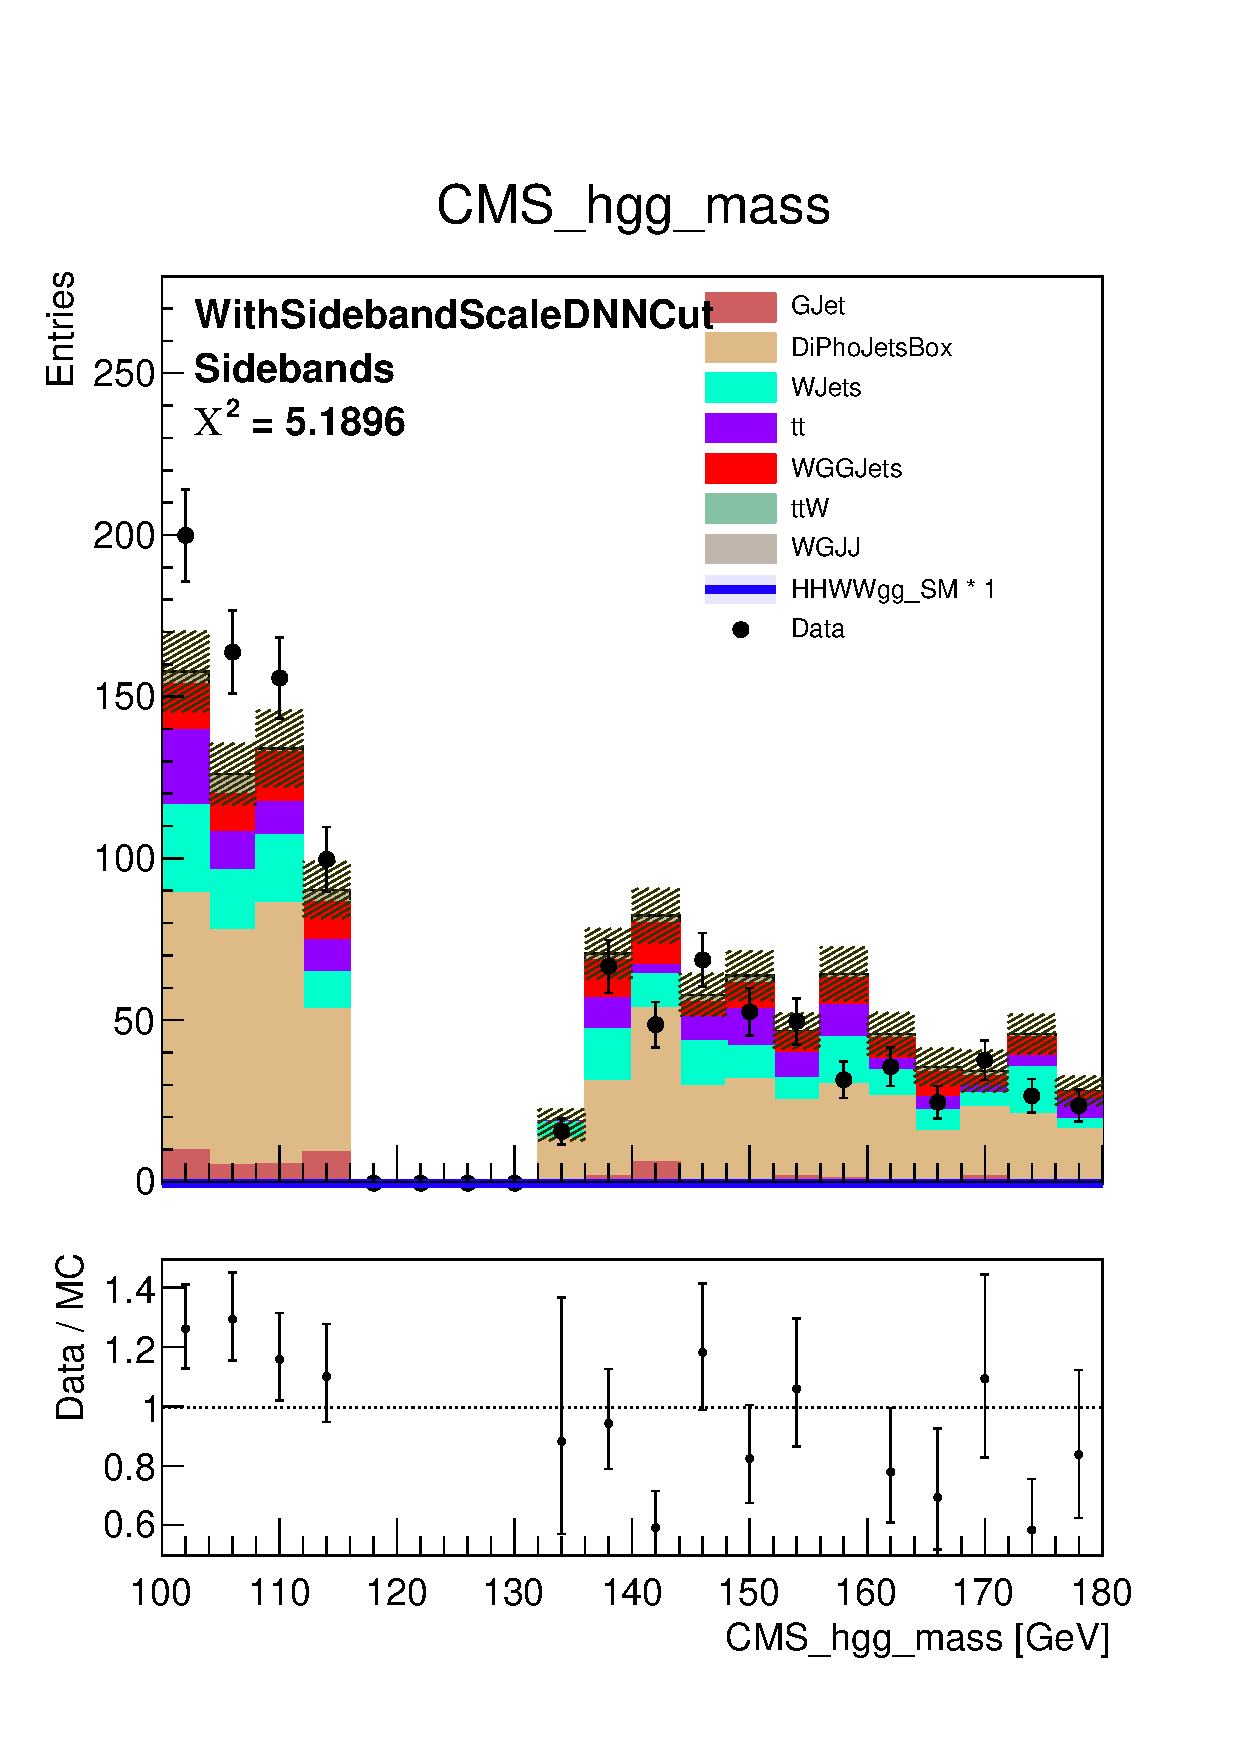
\includegraphics[width=0.45\textwidth]{Sections/HHWWgg/images/DNN/DataMC_CMS_hgg_mass_SB_WithSidebandScaleFactor_nonLog.pdf}}
%   \caption{data / MC ratio of DNN output score in the data sidebands before and after applying a sideband integral scaling factor of 1.140 to MC}
%   \label{fig:DNNSidebands_withAndWithoutSidebandScale}
% \end{figure} 

\clearpage 

\subsubsection{Standard Model: Categorization} \label{subsubsec:SLCategorization}

After computing a DNN output score for each event, events are placed into categories based on their DNN score in order to maximize the sensitivity of the DNN categorization. The optimization of categories 
is done using the output HH class DNN score only, as it has a known correlation to the H and continuum background DNN scores. If an event has a large HH class DNN score, by construction 
it must have small H and continuum background DNN output scores. 
Sensitivity is maximized by systematically determining the ideal position of category boundaries in terms of DNN score in order to maximize total significance, a 
proxy of the result of the asymptotic limits method to be applied during extraction of final results via fitting of the background models to the data.

This categorization is done using signal and background MC in the signal region,
and therefore is maximally optimial for data when data and MC fully agree in the dataside bands. After scaling MC in the sidebands to the integral of data in the sidebands, a non-optimal data-MC agreement is found. In order to correct for this disagreement, 
a per-bin reweighting of the DNN score is performed. The reweighting is performed using the Run 2 dataset and 2017 MC, with MC appropriately scaled to cross section, luminosity, 
PU reweight and any CMS POG (Physics object groups) recommended scale factors. Each DNN score bin weight is computed as the ratio of data to MC in the sideband region. The event weight is then applied to MC 
in the sideband and signal region events. It should be noted that this reweighting is used only to optimize analysis categories, and is not used for the evaluation of 
any final results. %The reweighted DNN score distributions is used to compute a per-event weight. 

During category optimization, generally a finner binning of the DNN score distributions leads to a greater significance. However, small bin widths can cause statistical fluctuations which 
bias categorization, as a very high (low) yield bin would improve (reduce) a potential category's significance drastically, thus biasing the categorization. To ensure that the 
effect of statistical fluctuations is reduced in the categorization procedure, a smoothing of the background distributions is performed. %using the Smooth-Super method of TGraphSmooth.

% The result of this smoothing can be seen in Figure \ref{fig:DNN-Smoothing}, where the median red line is used as the background distribution for categorization. In addition, 
% a $\pm 1\sigma$ Poissonian uncertainty is applied bin-by-bin to the smoothed distribution. This is done in order to demonstrate that most fluctuations are Poissonian in nature. 

The smoothing procedure is performed on background MC in the signal and side-band region. The smoothing procedure ensures that statistical fluctuations in the shape of the 
DNN scores have a negligible impact on the categorization procedure. 

% Events in the DNN discriminant distribution are separated into groups of bins ranging from DNN discriminant scores of 0.1 to 1. Events with a score of less than 0.1 are 
% not used for categorization. 

An optimal categorization of events based on the DNN discriminant variable is extracted by computing total significance among categories, varying the number of categories, number of equally sized bins, 
and definition of the signal region. A simultaneous optimization of category boundaries is performed, and the case which yields the greatest significance is chosen as the final categorization. Total significance is defined as the quadtratic sum of category 
significance, where category significance is defined by 
Equation \ref{eq:SignifianceDef} (Equation 96 in \cite{Cowan_2011}), where S and B are the number of weighted signal (HH events) and background (Single H $+$ continuum background) events in the category, respectively. Events with a score of less than 
0.1 are not used for categorization. 

\begin{equation} \label{eq:SignifianceDef}
  \sqrt{2((S + B)ln(1 + \frac{S}{B}) - S)}
\end{equation}

The optimal category boundaries for a given number of categories, equally sized bins and signal region window are chosen by computing total significance for every possible position of category boundaries 
given the number of bins and categories. A simultaneous optimization of category boundaries is performed. The category boundary positions which yield the greatest total significance are defined as the optimal category boundaries for the given number of categories,
bins and signal region window. 

The number of categories is varied from 1-5, and the number of equally sized bins is varied among: [10, 20, 30, 40, 50, 60, 70, 80, 90, 100, 110, 120, 130, 140, 150, 160, 170, 180, 190, 380, 760, 1520]. When computing significance 
values for category optimization, a signal region definition of 122 to 128 GeV is used as this is the experimental resolution: A range centered around the expected higgs mass with a width $\approx \pm$ 1-2 times the expected signal width,
known a-posteriori from analytic fitting. 

%, and the signal region window is varied
%among diphoton mass windows of (115, 135), (120, 130), (121, 129), (122, 128), and (123, 127). The signal region definition is varied because the significance computed in the di-photon mass range 115-135 may 
%not serve as the best proxy for the 95\% CL limit on di-Higgs cross section. 

The optimal categorization was chosen based on the 90 bin case, in which category boundaries are simultaneously optimized among 90 equally sized bins of width (1/90) from output DNN scores 
of 0.1 to 1. 

%It was also found that a signal region definition of 122 to 128 GeV in the di-photon mass region returns the greatest significance with number of bins and categories held constant,
%a hint that choosing optimal category boundaries based on this definiton may return the most sensitive result. 

% The expected signal region yields for background (simulated with MC reweighted to the data sidebands) and HH signal, both scaled to the Run 2 luminosity of 137 $fb^{-1}$, are shown in Figure \ref{fig:DnnScore} for the HH node DNN score. These distributions are 
% used for significance computations.    

A very small increase in total significance is obtained when increasing from four to five total categories, as seen in Figure \ref{fig:SigVsNcats}, in both the case where significance is computed with Equation \ref{eq:SignifianceDef}
and S / $\sqrt{B}$. In addition, the category boundary 
for the most sensitive category remains constant. Therefore, the choice is made to classify events into four categories. The category boundaries, number of signal events, number of background 
events and significance for the N category case where N ranges from 1-5 are shown in Tables \ref{tab:SLcategories_1}, \ref{tab:SLcategories_2}, \ref{tab:SLcategories_3}, \ref{tab:SLcategories_4} and \ref{tab:SLcategories_5},
where the final categorization is that shown in Table \ref{tab:SLcategories_4}. The HH yields in these tables, denoted by 'S', are properly scaled to the cross section and branching ratio of 
the Semi-Leptonic final state of HH$\rightarrow$WW$\gamma\gamma$. The MC modeling the backgound in the signal region comes from the continuum background MC which is smoothed before 
use in the category optimization. Each MC process is scaled to its cross section and branching ratio, as well as the kinematic weight with its fiducial selection, the removal of events with an absolute value of weight times kinematic 
weight $> 10$.

\newpage 

\begin{table}[H]
  \begin{center}
    \begin{tabular}{c|c|c|c|c|c|c}
    CatN & DNN Min & DNN Max & S & $B_{SR}$ & $Data_{Sideband}$ & Significance\\ \hline
    0 & 0.89 & 1.0 & 0.03568 & 0.81037 & 8.0 & 0.03935 \\ 
    \end{tabular}
  \end{center}
\caption{
    Semi-Leptonic DNN Category Boundaries and yields in signal region for 1 Categories
}
\label{tab:SLcategories_1}
\end{table}
 
\begin{table}[H]
  \begin{center}
    \begin{tabular}{c|c|c|c|c|c|c}
    CatN & DNN Min & DNN Max & S & $B_{SR}$ & $Data_{Sideband}$ & Significance\\ \hline
    0 & 0.89 & 1.0 & 0.03568 & 0.81037 & 8.0 & 0.03935 \\ 
    1 & 0.1 & 0.89 & 0.23129 & 511.65079 & 3580.0 & 0.01022 \\ 
    \end{tabular}
  \end{center}
\caption{
    Semi-Leptonic DNN Category Boundaries and yields in signal region for 2 Categories
}
\label{tab:SLcategories_2}
\end{table}
 
\begin{table}[H]
  \begin{center}
    \begin{tabular}{c|c|c|c|c|c|c}
    CatN & DNN Min & DNN Max & S & $B_{SR}$ & $Data_{Sideband}$ & Significance\\ \hline
    0 & 0.89 & 1.0 & 0.03568 & 0.81037 & 8.0 & 0.03935 \\ 
    1 & 0.64 & 0.89 & 0.09449 & 16.43561 & 114.0 & 0.02329 \\ 
    2 & 0.1 & 0.64 & 0.1368 & 495.21518 & 3466.0 & 0.00615 \\ 
    \end{tabular}
  \end{center}
\caption{
    Semi-Leptonic DNN Category Boundaries and yields in signal region for 3 Categories
}
\label{tab:SLcategories_3}
\end{table}
 
\begin{table}[H]
  \begin{center}
    \begin{tabular}{c|c|c|c|c|c|c}
    CatN & DNN Min & DNN Max & S & $B_{SR}$ & $Data_{Sideband}$ & Significance\\ \hline
    0 & 0.89 & 1.0 & 0.03568 & 0.81037 & 8.0 & 0.03935 \\ 
    1 & 0.84 & 0.89 & 0.02267 & 1.84053 & 12.0 & 0.01668 \\ 
    2 & 0.63 & 0.84 & 0.07483 & 15.73924 & 111.0 & 0.01885 \\ 
    3 & 0.1 & 0.63 & 0.13379 & 494.07101 & 3457.0 & 0.00602 \\ 
    \end{tabular}
  \end{center}
\caption{
    Semi-Leptonic DNN Category Boundaries and yields in signal region for 4 Categories
}
\label{tab:SLcategories_4}
\end{table}
 
\begin{table}[H]
  \begin{center}
    \begin{tabular}{c|c|c|c|c|c|c}
    CatN & DNN Min & DNN Max & S & $B_{SR}$ & $Data_{Sideband}$ & Significance\\ \hline
    0 & 0.89 & 1.0 & 0.03568 & 0.81037 & 8.0 & 0.03935 \\ 
    1 & 0.84 & 0.89 & 0.02267 & 1.84053 & 12.0 & 0.01668 \\ 
    2 & 0.64 & 0.84 & 0.07182 & 14.59508 & 102.0 & 0.01878 \\ 
    3 & 0.25 & 0.64 & 0.0964 & 157.99225 & 974.0 & 0.00767 \\ 
    4 & 0.1 & 0.25 & 0.0404 & 337.22293 & 2492.0 & 0.0022 \\ 
    \end{tabular}
  \end{center}
\caption{
    Semi-Leptonic DNN Category Boundaries and yields in signal region for 5 Categories
}
\label{tab:SLcategories_5}
\end{table}

\newpage 

\begin{figure}[H]
  \setlength{\unitlength}{1mm}
  \begin{center}
    \mbox{\includegraphics*[height=100mm]{Sections/HHWWgg/images/DNN/Categorization/SigVsNCats.pdf}
    }
  \end{center}
  \caption{Total significance vs. number of categories in DNN categorization optimization, using either Equation \ref{eq:SignifianceDef} or S / $\sqrt{B}$ to 
  compute each category's significance, with total significance computed as category significances summed in quadrature. S is the number of weighted HH events, 
  and B is the weghted number of MC events modeling the continuum background in the signal region plus the number of weighted single H events. Also shown in Table \ref{tab:SigVsNcats_table}}    
  \label{fig:SigVsNcats}
\end{figure}

\begin{table}[H]
  \begin{center}
    \begin{tabular}{c|c|c}
    NCategories & Total Significance with Eq \ref{eq:SignifianceDef} & $\frac{S}{\sqrt{B}}$ \\ \hline
    1 & 0.03935 & 0.039635  \\ 
    2 & 0.040656 & 0.040933  \\ 
    3 & 0.046135 & 0.04639  \\ 
    4 & 0.047095 & 0.047352  \\ 
    5 & 0.04736 & 0.047616  \\ 
    \end{tabular}
  \end{center}
\caption{
    Significance values using two equations for significance
}
\label{tab:SigVsNcats_table}
\end{table}

\clearpage

\subsubsection{EFT Benchmarks: Parametric Binary Deep Neural Network}

To categorize events from the 20 EFT benchmarks in the Semi-Leptonic final state, a parametric binary DNN is used. The DNN is trained using 2017 signal and background samples, and 
is evaluated on 2016, 2017 and 2018 signal samples for analytic fitting and on Run 2 data to be used for categorization and data-driven background modeling. 
Models of the 20 EFT benchmarks are obtained by reweighting the combination of four NLO samples to each benchmark at NLO precision. The 20 EFT benchmark samples are combined and considered together as signal. 
The network is then trained on a labelled dataset with the 20 EFT HH processes as the signal, 
and various background process labelled as background. 

In addition to the training variables used for the multiclass DNN, the node number ranging from 1-20 is input as a feature into the DNN, allowing one to produce an output score for 
any EFT benchmark hypothesis. This is essentially a way to produce 20 MVA scores in a given training, which is much more convenient than running 20 individual trainings.

% The samples used for training and labeled as signal are the 12 LO benchmark samples with 2017 detector conditions. When training on these samples, the same reweighting 
% procedure described in the multi-class DNN is followed, where in this case samples are reweighted to the NLO precision of their corresponding benchmark rather than 
% the standard model at NLO precision. 

The same training pre-selections are applied in this case as for the multi-class DNN, and the same category boundary optimization procedure is followed. 